\documentclass[12pt,a4paper]{report}
\usepackage[utf8]{inputenc}
\usepackage{graphicx}
\usepackage[a4paper,left=3.5cm,right=1.25cm,top=2.5cm,bottom=1.25cm]{geometry}
\usepackage{setspace}
\usepackage{times}
\usepackage{titlesec}
\usepackage{float}
\usepackage{caption}
\usepackage{hyperref}
\usepackage{booktabs}
\usepackage{array}
\usepackage{longtable}
\usepackage{fancyhdr}
\usepackage{enumitem}
\usepackage{xcolor}
\usepackage{tikz}
\usetikzlibrary{shapes.geometric,arrows.meta,positioning,calc,fit,backgrounds}
\definecolor{primaryblue}{HTML}{6366F1}
\definecolor{accentcyan}{HTML}{06B6D4}
\definecolor{successgreen}{HTML}{22C55E}
\definecolor{warningamber}{HTML}{F59E0B}
\definecolor{bordercolor}{HTML}{252840}
\doublespacing
\pagestyle{fancy}
\fancyhf{}
\fancyfoot[C]{\thepage}
\renewcommand{\headrulewidth}{0pt}
\setlength{\footskip}{1.5cm}
\fancypagestyle{plain}{\fancyhf{}\fancyfoot[C]{\thepage}\renewcommand{\headrulewidth}{0pt}}
\begin{document}


\begin{titlepage}
\begin{spacing}{1.0}
\centering
\thispagestyle{empty}
\vspace*{0.8cm}

{\fontsize{30pt}{36pt}\selectfont\bfseries Academic Status Transparency\\[0.2cm]Notification System}\\[0.5cm]

{\fontsize{14pt}{18pt}\selectfont\bfseries MINOR PROJECT REPORT}\\[0.5cm]

{\fontsize{12pt}{14pt}\selectfont SUBMITTED IN PARTIAL FULFILMENT OF THE REQUIREMENTS FOR THE AWARD OF THE DEGREE OF}\\[0.4cm]

{\fontsize{14pt}{18pt}\selectfont\textbf{BACHELOR OF TECHNOLOGY}\\[0.2cm]Computer Science and Engineering}\\[0.5cm]


\includegraphics[width=0.40\textwidth]{assets/image.png}\\[0.5cm]

SUBMITTED BY\\[0.4cm]

\begin{center}
\begin{minipage}[t]{0.3\textwidth}
\centering
{\fontsize{13}{15}\selectfont ARSHDEEP ANAND}\\[0.1cm]
{\fontsize{11}{13}\selectfont URN: 2302481}\\[0.1cm]
{\fontsize{11}{13}\selectfont CRN: 2315025}
\end{minipage}
\hfill
\begin{minipage}[t]{0.3\textwidth}
\centering
{\fontsize{13}{15}\selectfont NISHTHA JAIN}\\[0.1cm]
{\fontsize{11}{13}\selectfont URN: 2302627}\\[0.1cm]
{\fontsize{11}{13}\selectfont CRN: 2315172}
\end{minipage}
\hfill
\begin{minipage}[t]{0.3\textwidth}
\centering
{\fontsize{13}{15}\selectfont BALKRISHAN SINGH}\\[0.1cm]
{\fontsize{11}{13}\selectfont URN: 2302492}\\[0.1cm]
{\fontsize{11}{13}\selectfont CRN: 2315036}
\end{minipage}\\[0.5cm]

{\fontsize{14}{16}\selectfont UNDER THE GUIDANCE OF}\\[0.15cm]
{\fontsize{14}{16}\selectfont Dr. Kapil Sharma}
\end{center}

\vspace{0.5cm}
{\fontsize{14pt}{18pt}\selectfont\bfseries DEPARTMENT OF COMPUTER SCIENCE AND ENGINEERING\\[0.2cm]GURU NANAK DEV ENGINEERING COLLEGE\\[0.2cm]LUDHIANA -- 141006}\\[0.3cm]
{\fontsize{12pt}{14pt}\selectfont MAY, 2026}

\end{spacing}
\end{titlepage}


\pagenumbering{roman}
\newpage
\begin{center}{\fontsize{16pt}{18pt}\selectfont\textbf{CERTIFICATE}}\end{center}
\vspace{1cm}
\noindent This is to certify that the minor project report entitled \textbf{``Academic Status Transparency Notification System''} is a bona fide record of the project work carried out by \textbf{Arshdeep Anand (URN: 2302481), Nishtha Jain (URN: 2302627), and Balkrishan Singh (URN: 2302492)} under my supervision and guidance, in partial fulfillment of the requirements for the award of the degree of Bachelor of Technology in Computer Science and Engineering from Guru Nanak Dev Engineering College, Ludhiana, affiliated to I.K. Gujral Punjab Technical University, Kapurthala. The work embodied in this report has not been submitted elsewhere for the award of any other degree or diploma to the best of my knowledge and belief.

\vspace{3cm}
\noindent\textbf{Dr. Kapil Sharma}\\
Assistant Professor\\
Department of Computer Science and Engineering\\
Guru Nanak Dev Engineering College, Ludhiana

\vspace{2cm}
\noindent\textbf{Dr. Kiran Jyoti}\\
Head of Department\\
Department of Computer Science and Engineering\\
Guru Nanak Dev Engineering College, Ludhiana


\newpage
\begin{center}{\fontsize{16pt}{18pt}\selectfont\textbf{ABSTRACT}}\end{center}
\noindent
The \textbf{Academic Status Transparency Notification System} (ASTNS) is a full-stack web application built to bridge the communication gap between engineering colleges affiliated to I.K. Gujral Punjab Technical University (IKGPTU) and the parents/guardians of enrolled students. In the prevailing academic ecosystem, result data is published on university portals but parents often remain unaware of their ward's detention status, declining semester grade point averages (SGPA), or poor subject-wise performance until it is too late for timely corrective intervention.

ASTNS eliminates this information asymmetry by automating the entire academic notification pipeline. Administrators at the institution log into a secure dashboard, upload bulk academic data via CSV or Excel files, review the parsed student records, and dispatch personalised email notifications. Each email contains a unique, cryptographically generated, time-limited hyperlink. Clicking the link opens the Guardian Portal -- a read-only, token-authenticated dashboard that presents the student's complete academic profile: semester-wise marks, internal and external scores per subject, SGPA trend chart, attendance indicator, and detention flags, all rendered without any login requirement for the guardian.

The system is implemented using the MERN stack: React 19 with Vite and Tailwind CSS on the frontend, Express.js 5 on the backend, and MongoDB Atlas as the cloud database. Email delivery is handled by Nodemailer over Gmail SMTP. The entire application is deployed serverlessly on Vercel.

Key contributions of the project include: (1) a drag-and-drop bulk upload interface with real-time data preview, (2) a cryptographic token lifecycle management module that tracks active, expired, and revoked access tokens, (3) an interactive line chart for visualising SGPA trends across semesters, and (4) a responsive Guardian Dashboard accessible on any device without requiring a guardian account.

System testing covered authentication, CSV parsing, notification dispatch, token validation, token revocation, chart rendering, and cross-browser compatibility. All major test cases passed successfully. The application demonstrates that modern web technologies can significantly improve academic transparency and parental engagement in higher education institutions.


\newpage
\begin{center}{\fontsize{16pt}{18pt}\selectfont\textbf{ACKNOWLEDGEMENT}}\end{center}
\noindent
We are highly grateful to Dr. Sehijpal Singh, Principal, Guru Nanak Dev Engineering College (GNDEC), Ludhiana, for providing us this opportunity to carry out the minor project work.

The constant guidance and encouragement received from Dr. Kiran Jyoti, Head of Department, CSE, GNDEC Ludhiana, has been of great help in carrying out the project work and is acknowledged with reverential thanks.

We would like to express a deep sense of gratitude and thanks profusely to our Project Guide, \textbf{Dr. Kapil Sharma}, Assistant Professor, Department of CSE, GNDEC Ludhiana; without his wise counsel and able guidance, it would have been impossible to complete the project in this manner.

We also express gratitude to other faculty members of the Department of Computer Science and Engineering of GNDEC for their intellectual support throughout the course of this work. Finally, we are indebted to all who have contributed to this report.

\vspace{1cm}
\noindent\textbf{Arshdeep Anand} \hfill URN: 2302481\\
\noindent\textbf{Nishtha Jain} \hfill URN: 2302627\\
\noindent\textbf{Balkrishan Singh} \hfill URN: 2302492\\

\newpage
\begin{center}{\fontsize{16pt}{18pt}\selectfont\textbf{LIST OF FIGURES}}\end{center}
\begin{table}[H]
\renewcommand{\arraystretch}{1.3}
\centering
{\fontsize{12pt}{14pt}\selectfont
\begin{tabular*}{\textwidth}{@{\extracolsep{\fill}} l >{\raggedright\arraybackslash}p{9cm} r}
\toprule
\textbf{Fig. No.} & \textbf{Figure Description} & \textbf{Page No.}\\
\midrule
3.1 & System Architecture Block Diagram & 16\\
3.2 & Level 0 DFD -- Context Diagram & 18\\
3.3 & Level 1 DFD & 19\\
3.4 & Use Case Diagram & 21\\
3.5 & Sequence Diagram -- Notification Flow & 22\\
3.6 & Activity Diagram -- Admin Workflow & 24\\
3.7 & Entity-Relationship (ER) Diagram & 26\\
3.8 & Frontend Component Architecture Diagram & 28\\
3.9 & Deployment Diagram & 29\\
3.10 & State Machine Diagram -- Token Lifecycle & 30\\
5.1 & Login Page & 52\\
5.2 & Admin Dashboard & 53\\
5.3 & Upload Data Page & 54\\
5.4 & Student List Page & 55\\
5.5 & Student Detail Page & 56\\
5.6 & Send Notification Page & 57\\
5.7 & Token Management Page & 58\\
5.8 & Guardian Dashboard -- Part 1 & 59\\
5.9 & Guardian Dashboard -- Part 2 & 60\\
5.10 & Access Denied Page & 61\\
5.11 & Email Notification Template & 62\\
\bottomrule
\end{tabular*}}
\end{table}

\newpage
\begin{center}{\fontsize{16pt}{18pt}\selectfont\textbf{LIST OF TABLES}}\end{center}
\begin{table}[H]
\renewcommand{\arraystretch}{1.3}
\centering
{\fontsize{12pt}{14pt}\selectfont
\begin{tabular*}{\textwidth}{@{\extracolsep{\fill}} l >{\raggedright\arraybackslash}p{9cm} r}
\toprule
\textbf{Table No.} & \textbf{Table Description} & \textbf{Page No.}\\
\midrule
2.1 & Software Requirements & 9\\
2.2 & Hardware Requirements & 10\\
2.3 & Functional Requirements & 11\\
2.4 & Non-Functional Requirements & 12\\
3.1 & Student Collection Schema & 25\\
3.2 & Subject Collection Schema & 26\\
3.3 & Token Collection Schema & 27\\
3.4 & Admin Collection Schema & 27\\
4.1 & REST API Endpoints -- Authentication & 37\\
4.2 & REST API Endpoints -- Students & 38\\
4.3 & REST API Endpoints -- Notifications & 39\\
4.4 & REST API Endpoints -- Tokens & 40\\
4.5 & Test Cases -- Authentication Module & 44\\
4.6 & Test Cases -- Data Upload Module & 45\\
4.7 & Test Cases -- Notification Module & 46\\
4.8 & Test Cases -- Guardian Portal & 47\\
\bottomrule
\end{tabular*}}
\end{table}

\newpage
\begin{center}{\fontsize{16pt}{18pt}\selectfont\textbf{TABLE OF CONTENTS}}\end{center}
\vspace{0.5cm}
\renewcommand{\arraystretch}{1.4}
{\fontsize{12pt}{14pt}\selectfont
\begin{longtable}{@{} l @{\hspace{1cm}} r @{}}
\textbf{Certificate} & \textbf{i}\\
\textbf{Abstract} & \textbf{ii}\\
\textbf{Acknowledgement} & \textbf{iii}\\
\textbf{List of Figures} & \textbf{iv}\\
\textbf{List of Tables} & \textbf{v}\\
\textbf{Table of Contents} & \textbf{vi}\\
\addlinespace[0.3cm]
\textbf{Chapter 1: Introduction} & \textbf{1}\\
\quad 1.1\quad Introduction to Project & 1\\
\quad 1.2\quad Project Category & 3\\
\quad 1.3\quad Problem Formulation & 3\\
\quad 1.4\quad Identification / Recognition of Need & 4\\
\quad 1.5\quad Existing System & 5\\
\quad 1.6\quad Objectives & 6\\
\quad 1.7\quad Proposed System & 7\\
\quad 1.8\quad Unique Features of the Proposed System & 8\\
\addlinespace[0.3cm]
\textbf{Chapter 2: Requirement Analysis and System Specification} & \textbf{9}\\
\quad 2.1\quad Feasibility Study & 9\\
\quad 2.2\quad Software Requirement Specification Document & 11\\
\quad 2.3\quad SDLC Model to be Used & 15\\
\addlinespace[0.3cm]
\textbf{Chapter 3: System Design} & \textbf{16}\\
\quad 3.1\quad Design Approach & 16\\
\quad 3.2\quad Detail Design & 17\\
\quad 3.3\quad User Interface Design & 31\\
\quad 3.4\quad Methodology & 34\\
\addlinespace[0.3cm]
\textbf{Chapter 4: Implementation and Testing} & \textbf{36}\\
\quad 4.1\quad Introduction to Languages, IDEs, Tools and Technologies & 36\\
\quad 4.2\quad Algorithm / Pseudocode & 41\\
\quad 4.3\quad Testing Techniques & 43\\
\quad 4.4\quad Test Cases & 44\\
\addlinespace[0.3cm]
\textbf{Chapter 5: Results and Discussions} & \textbf{51}\\
\quad 5.1\quad User Interface Representation & 51\\
\quad 5.2\quad Snapshots with Details & 52\\
\quad 5.3\quad Backend Database Representation & 63\\
\addlinespace[0.3cm]
\textbf{Chapter 6: Conclusion and Future Scope} & \textbf{65}\\
\addlinespace[0.3cm]
\textbf{References / Bibliography} & \textbf{68}\\
\textbf{Appendix A: Project Setup Guide} & \textbf{69}\\
\end{longtable}}

\newpage
\pagenumbering{arabic}
\setcounter{page}{1}

\chapter{Introduction}

\section{Introduction to Project}
The \textbf{Academic Status Transparency Notification System} (ASTNS) is a full-stack web application designed and developed to address a persistent problem in higher education institutions: the lack of timely, structured communication between colleges and the parents or guardians of enrolled students. The system targets engineering colleges affiliated with I.K. Gujral Punjab Technical University (IKGPTU), which serve thousands of students spread across numerous courses and branches.

In most institutions, academic results are published on the university's official portal. However, this portal requires students to actively check their marks, and there is no mechanism that directly informs parents or guardians about their ward's performance. Parents who are less tech-savvy, reside in rural areas, or are unfamiliar with university portals are effectively excluded from accessing this information. The consequences are severe: students with declining grades, attendance shortages, or detention status can conceal this information from their guardians until irreversible damage to their academic career has already occurred.

ASTNS resolves this by automating the complete pipeline from data entry to guardian notification. An institutional administrator logs into a secure, session-authenticated web dashboard. From there, the administrator can upload bulk student academic records from CSV or Excel files, review the parsed data in a preview table, and dispatch personalised email notifications with a single click. Each email contains a unique, cryptographically generated 32-character hex token embedded in a hyperlink. When the guardian clicks the link, the system validates the token and renders a dedicated Guardian Portal showing the student's full academic history.

The Guardian Portal displays: the student's name, university roll number, course, branch, semester-wise SGPA as an interactive line chart, detailed subject-wise marks tables for each semester (showing internal marks, external marks, total, and detention status per subject), an attendance ring indicator, and a button to download the report as a PDF. Crucially, guardians access all this without creating an account or remembering a password -- the token itself serves as the authentication credential.

The system is built using the MERN technology stack: React 19 with Vite as the build tool and Tailwind CSS 4 for styling on the frontend; Express.js 5 for the backend REST API; MongoDB Atlas as the cloud-hosted NoSQL database; and Nodemailer for SMTP-based email delivery. The application is deployed on Vercel as a serverless application.

The project was developed by a team of three students from the Department of Computer Science and Engineering, GNDEC Ludhiana, as part of the Minor Project requirement for the sixth semester of the B.Tech (CSE) programme.

\section{Project Category}
ASTNS is an \textbf{Application-Based} project. It is a production-ready, full-stack web application that solves a real-world institutional problem using modern web development technologies. The project does not involve theoretical research or hardware components; instead, it focuses on software engineering, system design, database management, RESTful API development, and user interface design.

The project can further be classified under the category of \textbf{Educational Technology (EdTech)} and \textbf{Institutional Communication Systems}.

\section{Problem Formulation}
The core problem addressed by ASTNS can be stated as follows:

\textit{There is no automated, secure, and accessible mechanism in most IKGPTU-affiliated engineering colleges for proactively communicating a student's academic status -- including detention flags, SGPA trends, and subject-wise performance -- to their parents or guardians.}

This problem has several dimensions:

\begin{itemize}
  \item \textbf{Information Asymmetry:} Students have access to their academic data, but parents do not unless the student chooses to share it.
  \item \textbf{Portal Complexity:} The university portal requires valid login credentials and technical familiarity, making it inaccessible to many parents.
  \item \textbf{Delayed Intervention:} By the time parents learn about their ward's academic difficulties, the student may have already been officially detained or failed multiple subjects.
  \item \textbf{No Aggregated View:} Even if a parent accesses the university portal, results are displayed per subject and per semester without any aggregated summary, trend analysis, or visual representation.
  \item \textbf{Administrative Burden:} Generating and sending individual academic reports manually is highly time-consuming for faculty and administrative staff.
\end{itemize}

These problems collectively result in reduced parental engagement, lower student accountability, and avoidable academic failures.

\section{Identification / Recognition of Need}
The need for a system like ASTNS was identified through the following observations:

\begin{enumerate}
  \item Engineering colleges under IKGPTU publish provisional results and attendance statements on the university portal, but these are not pushed to parents automatically.
  \item Detention is a critical academic consequence: a student detained in internal exams cannot appear in the university (external) examination, severely affecting their academic year. Parents are often unaware of this until after the examination period.
  \item Research in educational communication systems (Benablo et al., 2014) demonstrates that push-based notification systems -- systems that proactively send information to parents rather than requiring parents to pull the information -- significantly improve parental awareness and student accountability.
  \item HCI research indicates that complex login mechanisms reduce user engagement. A password-less access mechanism using secure deep-link tokens removes friction and increases the likelihood that guardians will actually view the shared reports.
  \item The increasing penetration of smartphones and email access in semi-urban and rural India makes an email-based notification system feasible even for parents outside major cities.
\end{enumerate}

\section{Existing System}
The existing mechanisms for academic communication in IKGPTU-affiliated colleges are as follows:

\begin{itemize}
  \item \textbf{University Portal:} Students and registered users can view results and attendance on the IKGPTU portal. However, parents must independently register and navigate the portal, which has low usability for non-technical users.
  \item \textbf{Physical Parent-Teacher Meetings (PTMs):} Colleges organise PTMs periodically, but these are infrequent, time-consuming, and often poorly attended.
  \item \textbf{Physical Letters or SMS:} Some colleges send bulk SMS alerts for attendance shortage or detention, but these are brief, lack detail, and provide no academic context.
  \item \textbf{Manual Report Cards:} Some institutions print result cards and send them home with students, but this is easily intercepted and is not reliable.
  \item \textbf{Generic ERP Portals:} A few institutions have subscribed to third-party ERP systems that include parent portals, but these require parents to create and maintain accounts, which reduces adoption.
\end{itemize}

\textbf{Limitations of the Existing System:}
\begin{itemize}
  \item No direct, automated push of academic data to parents.
  \item High friction for parents to access information (requires account creation and login).
  \item No aggregated academic summaries or trend visualisation.
  \item Delayed communication leading to late parental intervention.
  \item Vulnerable to student-side interception (physical letters, manual sharing).
\end{itemize}

\section{Objectives}
The primary objectives of the ASTNS project are:

\begin{enumerate}
  \item To Design and develop a web-based Academic Status Transparency Notification System that enables administrators to upload student academic data in bulk via CSV/Excel formats.
  \item To Automatically notify guardians via email with secure, time-limited access links, providing a Guardian Dashboard for viewing detailed semester reports with visual analytics.
  \item To Implement a Token Management system ensuring secure, traceable access to student records.
\end{enumerate}

\section{Proposed System}
The proposed Academic Status Transparency Notification System (ASTNS) is a full-stack web application that digitises and automates the entire academic communication pipeline. The system operates as follows:

\textbf{Administrator Side:}
\begin{enumerate}
  \item The administrator logs into the secure Admin Dashboard using email and password credentials. Sessions are managed using server-side session storage and signed cookies.
  \item From the Upload Data module, the administrator selects the relevant course, branch, and semester, then uploads a CSV or Excel file containing student academic records.
  \item The system parses the file, validates each record against the database schema constraints (e.g., valid marks ranges, recognised course-branch combinations), and displays a preview of the parsed data for review.
  \item Upon confirmation, the records are saved to the MongoDB Atlas cloud database.
  \item From the Send Notification module, the administrator selects the students for whom notifications should be dispatched and configures the token expiry duration (24 hours, 48 hours, 72 hours, or 7 days).
  \item The system generates a unique 32-character hexadecimal token for each selected student using Node.js's \texttt{crypto} module, stores the token in the database with an expiry timestamp, constructs a personalised guardian portal URL, and dispatches an HTML email to the guardian's registered email address via Gmail SMTP.
  \item The administrator can monitor all generated tokens from the Token Management module, view their status (Active, Used, Expired), and manually revoke tokens if required.
\end{enumerate}

\textbf{Guardian Side:}
\begin{enumerate}
  \item The guardian receives an HTML email containing a ``View Report'' button linked to the Guardian Portal URL with the embedded token.
  \item Clicking the link opens the Guardian Portal in a browser. The system validates the token: if it is valid and active, the student's academic data is rendered; if it is expired or revoked, an Access Denied page is displayed.
  \item The guardian views the student's academic profile, SGPA trend chart, semester-wise mark breakdown, and detention indicators.
  \item The guardian can download the report as a PDF for record-keeping.
\end{enumerate}

\section{Unique Features of the Proposed System}
\begin{itemize}
  \item \textbf{Password-less Guardian Access:} Eliminates the need for guardians to create accounts or remember passwords. The token embedded in the email link is the sole authentication credential, dramatically reducing access friction.
  \item \textbf{Cryptographic Token Security:} Each access token is generated using \texttt{crypto.randomBytes(16)} in Node.js, producing a 32-character hexadecimal string that is computationally infeasible to guess or brute-force.
  \item \textbf{Configurable Token Expiry:} Administrators can set token validity to 24 hours, 48 hours, 72 hours, or 7 days, balancing security and convenience.
  \item \textbf{Bulk Data Upload with Preview:} Supports drag-and-drop CSV and Excel uploading with real-time parsing and a data preview table, allowing administrators to verify records before committing to the database.
  \item \textbf{Interactive SGPA Trend Chart:} Uses Recharts to render a responsive line chart of the student's SGPA across all semesters, providing a quick visual summary of academic trajectory.
  \item \textbf{Serverless Deployment:} The entire application (frontend SPA and backend API) is deployed on Vercel as serverless functions, ensuring zero infrastructure management and automatic scaling.
  \item \textbf{Multi-Course, Multi-Branch Support:} The system supports all IKGPTU courses (B.Tech, M.Tech, MBA, MCA, BCA, B.Arch, B.Voc, B.Com, BBA) and their respective branches through a centralised \texttt{courseBranchMap} validation utility.
\end{itemize}

\chapter{Requirement Analysis and System Specification}

\section{Feasibility Study}
A feasibility study evaluates whether the proposed system is practical, beneficial, and viable to develop. The ASTNS was evaluated across three dimensions of feasibility.

\subsection{Technical Feasibility}
The ASTNS is built entirely on the MERN stack -- MongoDB, Express.js, React, and Node.js -- which is one of the most widely adopted technology stacks for full-stack web applications. All components are open-source, well-documented, and have large, active developer communities.

\begin{itemize}
  \item \textbf{Frontend:} React 19 (with Vite 7 and Tailwind CSS 4) provides a component-driven, declarative UI framework. Recharts 3 is used for data visualisation. React Hook Form 7 handles form management and validation.
  \item \textbf{Backend:} Express.js 5 provides a minimal, flexible Node.js web framework for building the REST API. Mongoose 9 is used as the Object Document Mapper (ODM) for MongoDB.
  \item \textbf{Database:} MongoDB Atlas (M0 Free Tier) provides a fully managed, cloud-hosted NoSQL database with automatic scaling, backups, and a web-based management UI.
  \item \textbf{Email:} Nodemailer 8 integrates with Gmail SMTP to dispatch HTML emails. The \texttt{crypto} module (built into Node.js) is used for token generation.
  \item \textbf{Deployment:} Vercel provides serverless hosting for both the React SPA and the Express.js API. No server management is required.
\end{itemize}

The development team has proficiency in all the above technologies. The required tools (VS Code, Node.js, Git, MongoDB Compass, Postman) are freely available. The project is therefore technically feasible.

\subsection{Operational Feasibility}
The ASTNS is operationally feasible for the following reasons:

\begin{itemize}
  \item Institutional administrators already maintain student academic records in Excel or CSV formats. The system's bulk upload module is directly compatible with these existing workflows.
  \item The Admin Dashboard is designed for minimal training. An administrator unfamiliar with the system can learn to upload data and dispatch notifications within one session.
  \item Parents and guardians interact only with the Guardian Portal, which requires no technical knowledge -- simply clicking a link in an email and viewing the report.
  \item The email-based notification system leverages a communication channel (email) that is already widely used for institutional communication.
  \item The serverless deployment model ensures the system is always available without requiring dedicated IT staff to manage servers.
\end{itemize}

\subsection{Economic Feasibility}
The ASTNS is economically feasible because all components are either free or available on free-tier plans:

\begin{itemize}
  \item \textbf{MongoDB Atlas M0:} Free tier with 512 MB of storage, sufficient for a college with up to 5,000 students.
  \item \textbf{Vercel Hobby Plan:} Free for personal and academic projects, with support for serverless functions.
  \item \textbf{Gmail SMTP:} Free to use with a Gmail account (subject to daily sending limits of 500 emails per day, extendable with Google Workspace).
  \item \textbf{All frameworks and libraries:} Open-source and free.
\end{itemize}

Total development cost is essentially zero beyond the cost of development machines (already owned by the team) and internet connectivity.
\section{Software Requirement Specification Document}

\subsection{Software Requirements}

\begin{longtable}{|p{3.5cm}|p{4cm}|p{5cm}|}
\caption{Software Requirements} \\
\hline
\textbf{Category} & \textbf{Technology} & \textbf{Version / Details}\\
\hline
\endfirsthead
\multicolumn{3}{c}{{\bfseries \tablename\ \thetable{} -- continued from previous page}} \\
\hline
\textbf{Category} & \textbf{Technology} & \textbf{Version / Details}\\
\hline
\endhead
Runtime Environment & Node.js & v20.x LTS\\
\hline
Frontend Framework & React & 19.2.0\\
\hline
Build Tool & Vite & 7.3.1\\
\hline
CSS Framework & Tailwind CSS & 4.2.1\\
\hline
Data Visualisation & Recharts & 3.7.0\\
\hline
Form Management & React Hook Form & 7.71.2\\
\hline
HTTP Client & Axios & 1.13.6\\
\hline
Routing & React Router DOM & 7.13.1\\
\hline
Icon Library & Lucide React & 0.575.0\\
\hline
Backend Framework & Express.js & 5.2.1\\
\hline
Database & MongoDB Atlas & M0 Free Tier\\
\hline
ODM & Mongoose & 9.2.3\\
\hline
Email Service & Nodemailer & 8.0.1\\
\hline
Deployment Platform & Vercel & Serverless Functions\\
\hline
Version Control & Git + GitHub & Latest\\
\hline
IDE & VS Code & Latest\\
\hline
API Testing & Postman & Latest\\
\hline
Browser & Chrome, Firefox, Safari & Latest\\
\hline
OS & Windows / macOS & Development\\
\hline
\end{longtable}

\subsection{Hardware Requirements}

\begin{longtable}{|p{3.5cm}|p{9cm}|}
\caption{Hardware Requirements} \\
\hline
\textbf{Component} & \textbf{Minimum Specification}\\
\hline
\endfirsthead
\multicolumn{2}{c}{{\bfseries \tablename\ \thetable{} -- continued from previous page}} \\
\hline
\textbf{Component} & \textbf{Minimum Specification}\\
\hline
\endhead
Processor & Intel Core i5 (8th Gen or higher) / Apple M1 or equivalent\\
\hline
RAM & 8 GB (16 GB recommended for development)\\
\hline
Storage & 256 GB SSD\\
\hline
Network & Broadband Internet (required for MongoDB Atlas, SMTP, Vercel)\\
\hline
Display & 1366 $\times$ 768 resolution or higher\\
\hline
\end{longtable}

\subsection{Functional Requirements}

\begin{longtable}{|p{1cm}|p{3cm}|p{9cm}|}
\caption{Functional Requirements} \\
\hline
\textbf{FR\#} & \textbf{Module} & \textbf{Requirement}\\
\hline
\endfirsthead
\multicolumn{3}{c}{{\bfseries \tablename\ \thetable{} -- continued from previous page}} \\
\hline
\textbf{FR\#} & \textbf{Module} & \textbf{Requirement}\\
\hline
\endhead
FR1 & Authentication & The system shall allow administrators to log in using email and password. Sessions shall be maintained using signed HTTP cookies.\\
\hline
FR2 & Authentication & The system shall allow administrators to log out, invalidating the current session.\\
\hline
FR3 & Data Upload & The system shall accept CSV and Excel files for bulk upload of student academic records.\\
\hline
FR4 & Data Upload & The system shall validate uploaded records against schema constraints (valid marks, course-branch mapping) before persisting to the database.\\
\hline
FR5 & Data Upload & The system shall display a preview of parsed records for administrator review before final submission.\\
\hline
FR6 & Student Mgmt & The system shall display a searchable, filterable list of all students in the database.\\
\hline
FR7 & Student Mgmt & The system shall display a detailed academic profile for each student, including all semesters and subject marks.\\
\hline
FR8 & Notification & The system shall generate a unique cryptographic token for each selected student and persist it with an expiry timestamp.\\
\hline
FR9 & Notification & The system shall dispatch an HTML email to each guardian containing a personalised report link with the embedded token.\\
\hline
FR10 & Token Mgmt & The system shall display all generated tokens with their current status (Active, Used, Expired).\\
\hline
FR11 & Token Mgmt & The system shall allow administrators to manually revoke any active token.\\
\hline
FR12 & Guardian Portal & The system shall validate a provided token and render the student's academic report if the token is valid and active.\\
\hline
FR13 & Guardian Portal & The system shall display an Access Denied page if the token is expired, revoked, or invalid.\\
\hline
\end{longtable}

\subsection{Non-Functional Requirements}

\begin{longtable}{|p{2.5cm}|p{10cm}|}
\caption{Non-Functional Requirements} \\
\hline
\textbf{Category} & \textbf{Requirement}\\
\hline
\endfirsthead
\multicolumn{2}{c}{{\bfseries \tablename\ \thetable{} -- continued from previous page}} \\
\hline
\textbf{Category} & \textbf{Requirement}\\
\hline
\endhead
Security & All API routes (except token validation and guardian report) shall require an authenticated admin session. Tokens shall be generated using cryptographically secure random bytes.\\
\hline
Performance & The Guardian Portal shall load student data within 2 seconds under normal network conditions.\\
\hline
Scalability & The serverless deployment on Vercel shall automatically scale to handle concurrent guardian accesses during peak result announcement periods.\\
\hline
Reliability & The email dispatch module shall use \texttt{Promise.allSettled} to ensure that a failure for one student does not abort the entire batch notification.\\
\hline
Usability & The Guardian Portal shall require zero technical knowledge from the guardian -- clicking a hyperlink shall be the only required action.\\
\hline
Maintainability & All backend API routes shall follow a consistent RESTful naming convention. All frontend components shall be modular and reusable.\\
\hline
Compatibility & The Guardian Portal shall render correctly on Chrome, Firefox, Safari, and Edge on both desktop and mobile devices.\\
\hline
\end{longtable}
\newpage
\section{SDLC Model to be Used}
The project adopted the \textbf{Agile Software Development Life Cycle} model with iterative sprints. Each sprint lasted one week and focused on a specific deliverable. The rationale for choosing Agile over Waterfall or Spiral models is:

\begin{itemize}
  \item \textbf{Flexibility:} Requirements for the Guardian Portal evolved during development (e.g., adding the attendance ring indicator and PDF download features). Agile accommodated these changes without requiring a full redesign.
  \item \textbf{Incremental Delivery:} Each sprint produced a testable, working module (Authentication, Upload, Notification, Guardian Portal, Token Management, Dashboard), allowing continuous verification of functionality.
  \item \textbf{Early Bug Detection:} Testing at the end of each sprint ensured bugs were caught and fixed before they propagated to subsequent modules.
  \item \textbf{Team Coordination:} The three-member team divided work by frontend, backend, and integration responsibilities, with daily sync-up meetings to track progress.
\end{itemize}

\textbf{Sprint Breakdown:}
\begin{enumerate}
  \item Sprint 1 (Week 1): Requirement analysis, system design, database schema design.
  \item Sprint 2 (Week 2): Backend -- Admin model, authentication API, session management.
  \item Sprint 3 (Week 3): Backend -- Student and Subject models, data upload API.
  \item Sprint 4 (Week 4): Backend -- Notification API, token generation, email dispatch.
  \item Sprint 5 (Week 5): Backend -- Token management API, report/guardian API.
  \item Sprint 6 (Week 6): Frontend -- Login page, Admin Layout, Sidebar, Dashboard.
  \item Sprint 7 (Week 7): Frontend -- Upload Data, Student List, Student Detail pages.
  \item Sprint 8 (Week 8): Frontend -- Send Notification, Token Management pages.
  \item Sprint 9 (Week 9): Frontend -- Guardian Dashboard, Access Denied pages.
  \item Sprint 10 (Week 10): Integration testing, bug fixes, deployment to Vercel.
\end{enumerate}

\chapter{System Design}

\section{Design Approach}
ASTNS follows an \textbf{Object-Oriented Design} approach combined with \textbf{Component-Driven Architecture} on the frontend and \textbf{Layered RESTful Architecture} on the backend. The system is divided into clearly separated layers:

\begin{itemize}
  \item \textbf{Presentation Layer:} React components organised by feature (Admin pages, Guardian pages, shared components, layouts).
  \item \textbf{API Layer:} Express.js routes and controllers implementing RESTful endpoints.
  \item \textbf{Business Logic Layer:} Controller functions, Mongoose schema hooks (pre-validate, pre-save), and utility modules (token generation, email template, data parsing).
  \item \textbf{Data Layer:} MongoDB Atlas collections (Admin, Student, Subject, Token, Session).
\end{itemize}

The system is designed around two primary user roles:
\begin{enumerate}
  \item \textbf{Administrator:} Authenticated via session cookie. Has full access to the Admin Dashboard, including data upload, student management, notification dispatch, and token management.
  \item \textbf{Guardian:} Authenticated via URL token. Has read-only access to the Guardian Portal for their ward's academic data.
\end{enumerate}

\section{Detail Design}

\subsection{System Architecture}

The system architecture connects three main tiers: the client (browser), the server (Vercel serverless functions running Express.js), and the database/external services (MongoDB Atlas + Gmail SMTP).

\begin{figure}[H]
\centering
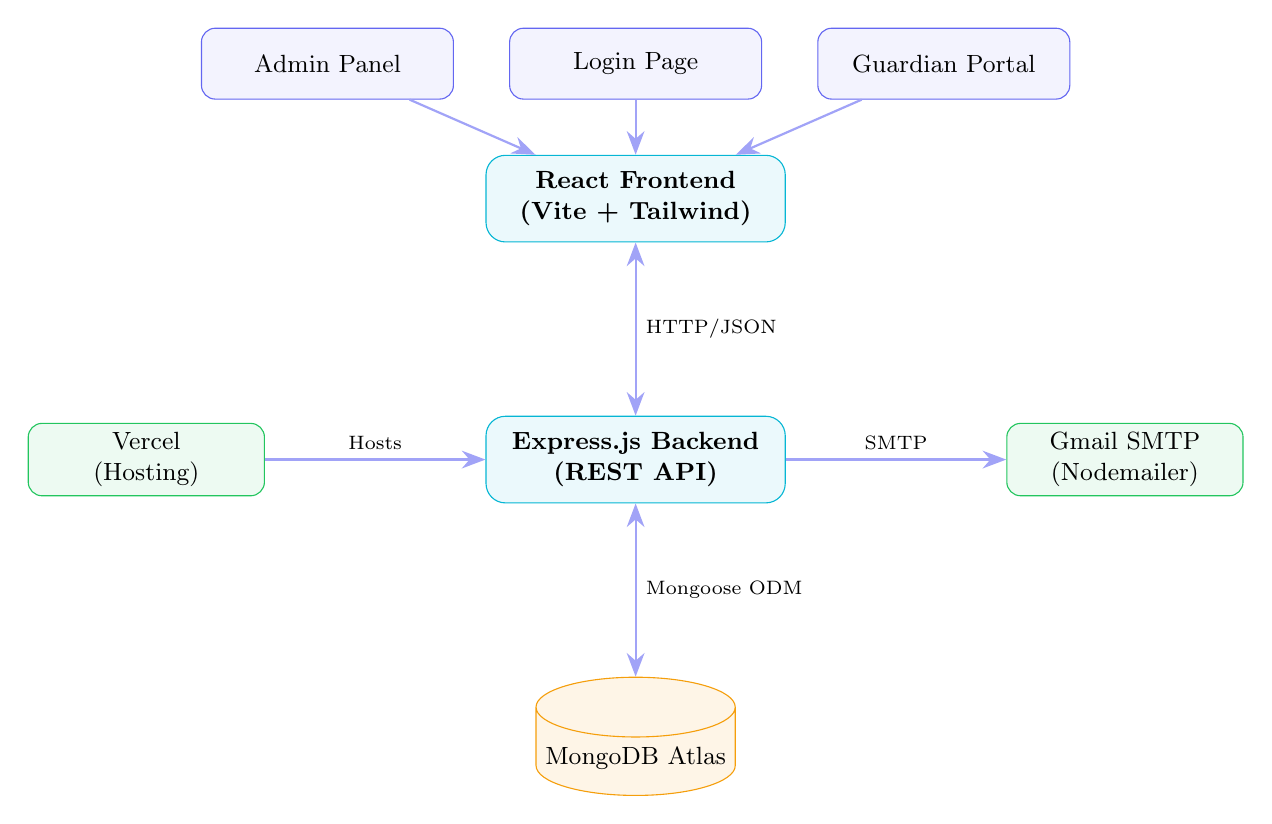
\begin{tikzpicture}[
  block/.style={rectangle,draw=primaryblue,fill=primaryblue!8,rounded corners=5pt,minimum width=3.2cm,minimum height=0.9cm,align=center,font=\small},
  bigblock/.style={rectangle,draw=accentcyan,fill=accentcyan!8,rounded corners=7pt,minimum width=3.8cm,minimum height=1.1cm,align=center,font=\small\bfseries},
  extblock/.style={rectangle,draw=successgreen,fill=successgreen!8,rounded corners=5pt,minimum width=3cm,minimum height=0.9cm,align=center,font=\small},
  dbblock/.style={cylinder,draw=warningamber,fill=warningamber!10,shape border rotate=90,minimum width=2.5cm,minimum height=1.3cm,aspect=0.3,align=center,font=\small},
  arr/.style={-{Stealth[length=3mm]},thick,draw=primaryblue!60},
  darr/.style={{Stealth[length=3mm]}-{Stealth[length=3mm]},thick,draw=primaryblue!60}
]
\node[bigblock] (fe) {React Frontend\\(Vite + Tailwind)};
\node[bigblock,below=2.2cm of fe] (be) {Express.js Backend\\(REST API)};
\node[dbblock,below=2.2cm of be] (db) {MongoDB Atlas};
\node[extblock,right=2.8cm of be] (smtp) {Gmail SMTP\\(Nodemailer)};
\node[extblock,left=2.8cm of be] (vercel) {Vercel\\(Hosting)};
\node[block,above left=0.7cm and 0.4cm of fe] (adm) {Admin Panel};
\node[block,above right=0.7cm and 0.4cm of fe] (grd) {Guardian Portal};
\node[block,above=0.7cm of fe] (login) {Login Page};
\draw[arr] (adm)--(fe); \draw[arr] (grd)--(fe); \draw[arr] (login)--(fe);
\draw[darr] (fe)--node[right,font=\scriptsize]{HTTP/JSON}(be);
\draw[darr] (be)--node[right,font=\scriptsize]{Mongoose ODM}(db);
\draw[arr] (be)--node[above,font=\scriptsize]{SMTP}(smtp);
\draw[arr] (vercel)--node[above,font=\scriptsize]{Hosts}(be);
\end{tikzpicture}
\caption{System Architecture Block Diagram}
\end{figure}

\subsection{Level 0 DFD -- Context Diagram}

The Level 0 DFD shows the system as a single process interacting with external entities.

\begin{figure}[H]
\centering
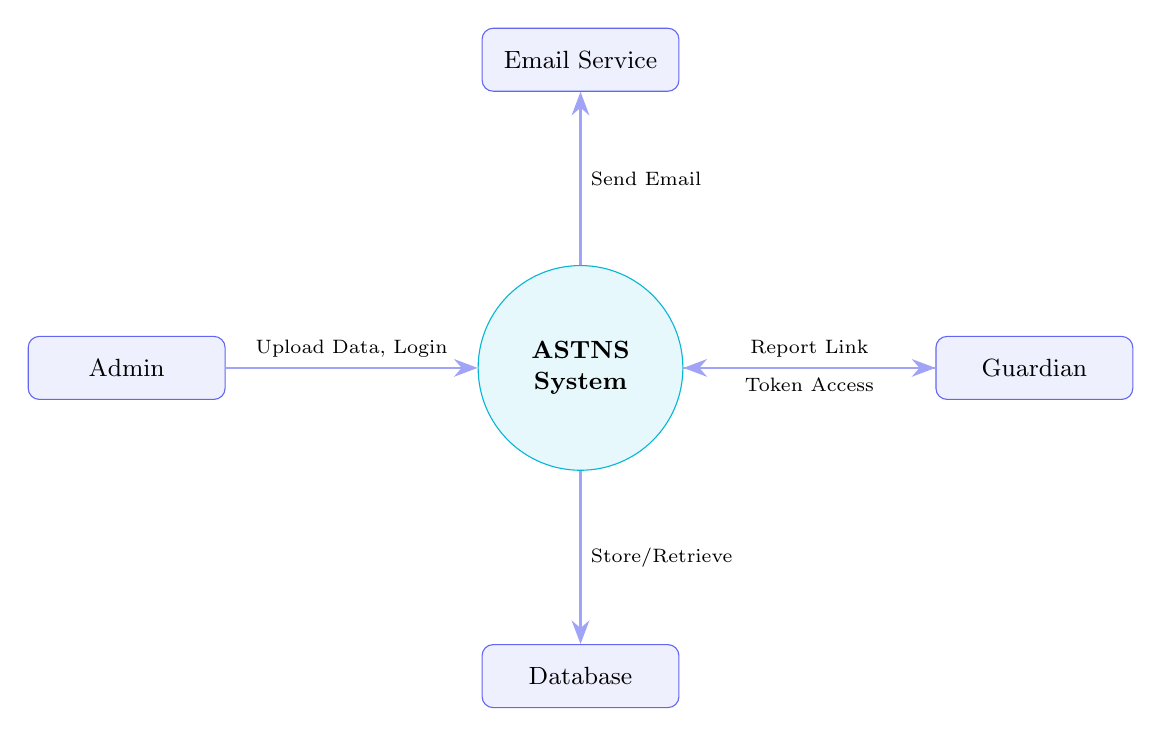
\begin{tikzpicture}[
  entity/.style={rectangle,draw=primaryblue,fill=primaryblue!10,rounded corners=4pt,minimum width=2.5cm,minimum height=0.8cm,align=center,font=\small},
  proc/.style={circle,draw=accentcyan,fill=accentcyan!10,minimum size=2.6cm,align=center,font=\small\bfseries},
  arr/.style={-{Stealth[length=3mm]},thick,draw=primaryblue!60}
]
\node[proc] (sys) {ASTNS\\System};
\node[entity,left=3.2cm of sys] (adm) {Admin};
\node[entity,right=3.2cm of sys] (grd) {Guardian};
\node[entity,below=2.2cm of sys] (db) {Database};
\node[entity,above=2.2cm of sys] (email) {Email Service};
\draw[arr] (adm)--node[above,font=\scriptsize]{Upload Data, Login}(sys);
\draw[arr] (sys)--node[above,font=\scriptsize]{Report Link}(grd);
\draw[arr] (grd)--node[below,sloped,font=\scriptsize]{Token Access}(sys);
\draw[arr] (sys)--node[right,font=\scriptsize]{Store/Retrieve}(db);
\draw[arr] (sys)--node[right,font=\scriptsize]{Send Email}(email);
\end{tikzpicture}
\caption{Level 0 DFD -- Context Diagram}
\end{figure}

\subsection{Level 1 DFD}

The Level 1 DFD decomposes the system into its major sub-processes.

\begin{figure}[H]
\centering
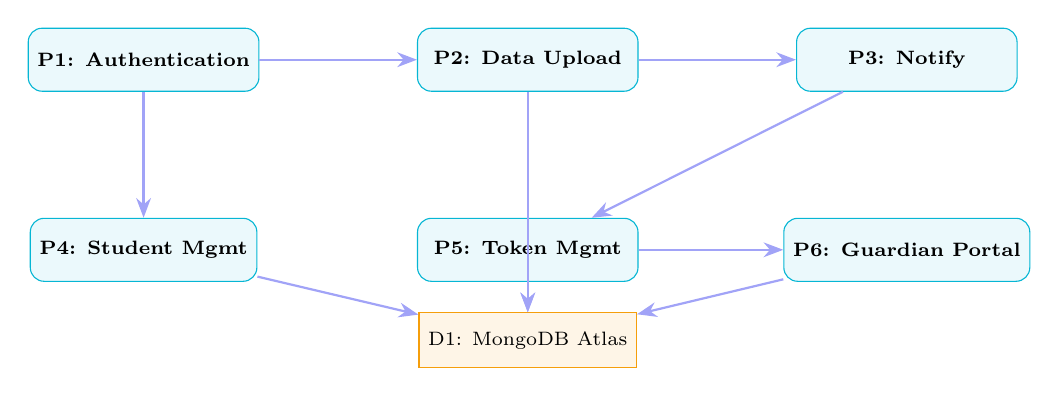
\begin{tikzpicture}[
  proc/.style={rectangle,draw=accentcyan,fill=accentcyan!8,rounded corners=5pt,minimum width=2.8cm,minimum height=0.8cm,align=center,font=\scriptsize\bfseries},
  store/.style={rectangle,draw=warningamber,fill=warningamber!10,minimum width=2.5cm,minimum height=0.7cm,align=center,font=\scriptsize},
  arr/.style={-{Stealth[length=2.5mm]},thick,draw=primaryblue!60},
  node distance=1.4cm
]
\node[proc] (auth) {P1: Authentication};
\node[proc,right=2cm of auth] (upload) {P2: Data Upload};
\node[proc,right=2cm of upload] (notif) {P3: Notify};
\node[proc,below=1.6cm of auth] (studmgmt) {P4: Student Mgmt};
\node[proc,below=1.6cm of upload] (tokenmgmt) {P5: Token Mgmt};
\node[proc,below=1.6cm of notif] (guardian) {P6: Guardian Portal};
\node[store,below=2.8cm of upload] (db) {D1: MongoDB Atlas};
\draw[arr] (auth)--(upload); \draw[arr] (upload)--(notif);
\draw[arr] (auth)--(studmgmt); \draw[arr] (notif)--(tokenmgmt);
\draw[arr] (tokenmgmt)--(guardian);
\draw[arr] (upload)--(db); \draw[arr] (studmgmt)--(db);
\draw[arr] (tokenmgmt)--(db); \draw[arr] (guardian)--(db);
\end{tikzpicture}
\caption{Level 1 DFD}
\end{figure}

\subsection{Use Case Diagram}

\begin{figure}[H]
\centering
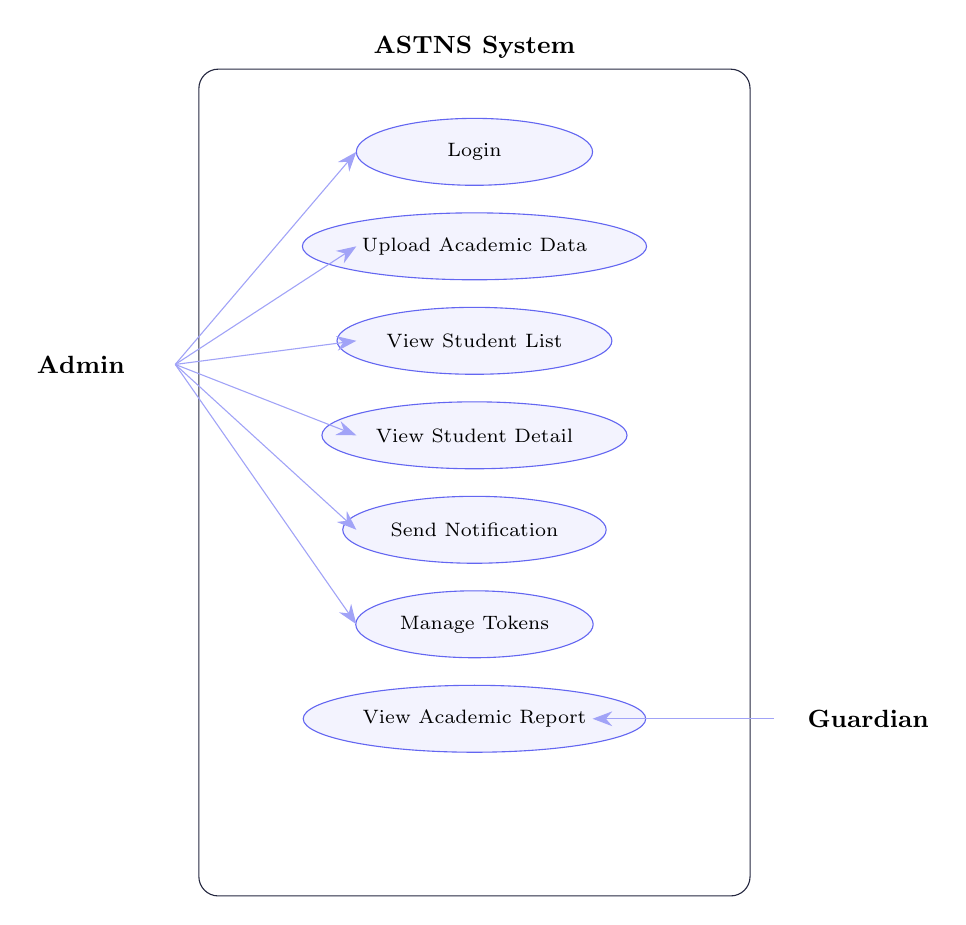
\begin{tikzpicture}[
  usecase/.style={ellipse,draw=primaryblue,fill=primaryblue!8,minimum width=3cm,minimum height=0.85cm,align=center,font=\scriptsize},
  arr/.style={-{Stealth[length=2.5mm]},draw=primaryblue!60},
  sysbox/.style={rectangle,draw=bordercolor,rounded corners=7pt,minimum width=7cm,minimum height=10.5cm}
]
\node[sysbox,label={[font=\small\bfseries]above:ASTNS System}] (sys) at (0,0){};
\node[usecase] at (0,4.2)  {Login};
\node[usecase] at (0,3.0)  {Upload Academic Data};
\node[usecase] at (0,1.8)  {View Student List};
\node[usecase] at (0,0.6)  {View Student Detail};
\node[usecase] at (0,-0.6) {Send Notification};
\node[usecase] at (0,-1.8) {Manage Tokens};
\node[usecase] at (0,-3.0) {View Academic Report};
\node[font=\small\bfseries] at (-5.0,1.5) {Admin};
\node[font=\small\bfseries] at (5.0,-3.0) {Guardian};
\foreach \uc in {4.2,3.0,1.8,0.6,-0.6,-1.8}
  \draw[arr] (-3.8,1.5)--(-1.5,\uc);
\draw[arr] (3.8,-3.0)--(1.5,-3.0);
\end{tikzpicture}
\caption{Use Case Diagram}
\end{figure}

\subsection{Sequence Diagram -- Notification Flow}

\begin{figure}[H]
\centering
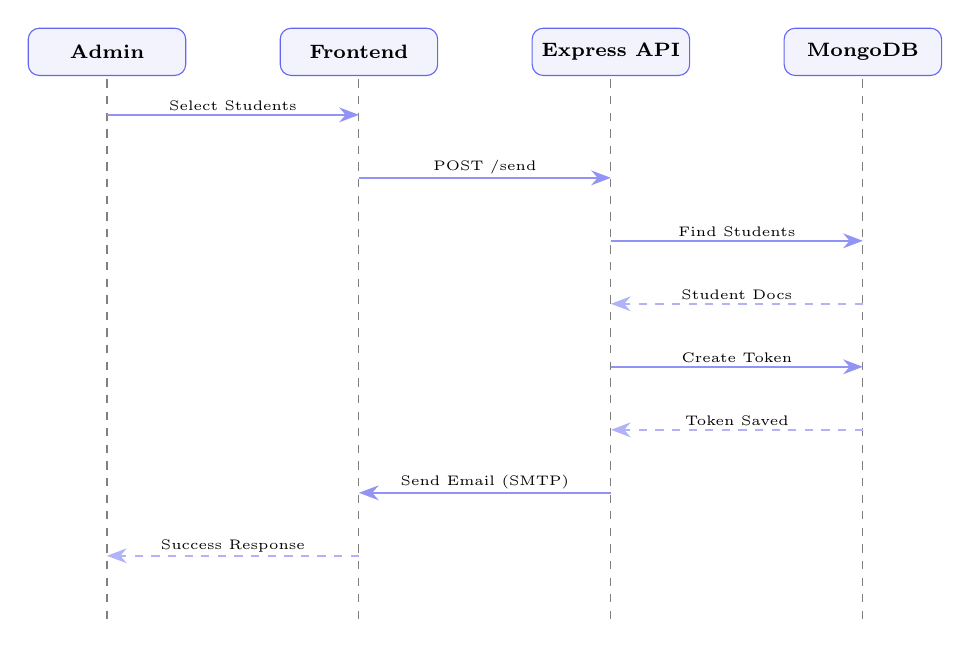
\begin{tikzpicture}[
  actor/.style={rectangle,draw=primaryblue,fill=primaryblue!8,rounded corners=4pt,minimum width=2cm,minimum height=0.6cm,align=center,font=\scriptsize\bfseries},
  arr/.style={-{Stealth[length=2.5mm]},thick,draw=primaryblue!70},
  darr/.style={-{Stealth[length=2.5mm]},thick,dashed,draw=primaryblue!50},
  lbl/.style={font=\tiny,fill=white,inner sep=1pt}
]
% Actors
\node[actor] (adm) at (0,0)   {Admin};
\node[actor] (ui)  at (3.2,0) {Frontend};
\node[actor] (api) at (6.4,0) {Express API};
\node[actor] (db)  at (9.6,0) {MongoDB};

% Lifelines
\foreach \x in {0,3.2,6.4,9.6}
  \draw[dashed,gray] (\x,-0.35)--(\x,-7.2);

% Arrows
\draw[arr]  (0,-0.8)  -- node[lbl,above]{Select Students}    (3.2,-0.8);
\draw[arr]  (3.2,-1.6) -- node[lbl,above]{POST /send}         (6.4,-1.6);
\draw[arr]  (6.4,-2.4) -- node[lbl,above]{Find Students}      (9.6,-2.4);
\draw[darr] (9.6,-3.2) -- node[lbl,above]{Student Docs}       (6.4,-3.2);
\draw[arr]  (6.4,-4.0) -- node[lbl,above]{Create Token}       (9.6,-4.0);
\draw[darr] (9.6,-4.8) -- node[lbl,above]{Token Saved}        (6.4,-4.8);
\draw[arr]  (6.4,-5.6) -- node[lbl,above]{Send Email (SMTP)}  (3.2,-5.6);
\draw[darr] (3.2,-6.4) -- node[lbl,above]{Success Response}   (0,-6.4);

\end{tikzpicture}
\caption{Sequence Diagram -- Notification Flow}
\end{figure}


\subsection{Activity Diagram -- Admin Workflow}

\begin{figure}[H]
\centering
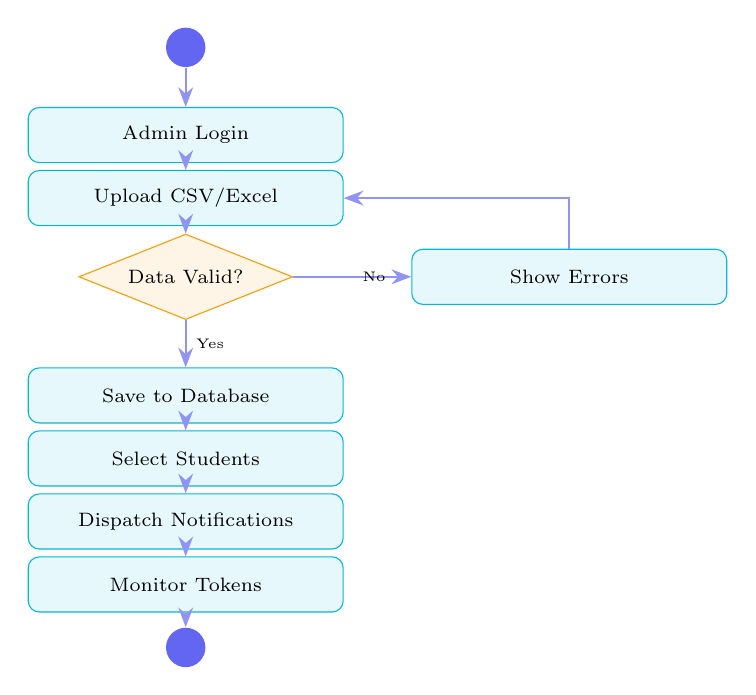
\begin{tikzpicture}[
  start/.style={circle,fill=primaryblue,minimum size=0.5cm},
  end/.style={circle,fill=primaryblue,minimum size=0.5cm,double,double distance=2pt},
  act/.style={rectangle,draw=accentcyan,fill=accentcyan!10,rounded corners=4pt,minimum width=4cm,minimum height=0.7cm,align=center,font=\scriptsize},
  dec/.style={diamond,draw=warningamber,fill=warningamber!10,aspect=2.5,font=\scriptsize},
  arr/.style={-{Stealth[length=2.5mm]},thick,draw=primaryblue!70},
  node distance=0.8cm
]
\node[start] (s) {};
\node[act,below=0.5cm of s] (login) {Admin Login};
\node[act,below of=login] (upload) {Upload CSV/Excel};
\node[dec,below of=upload,yshift=-0.2cm] (valid) {Data Valid?};
\node[act,right=1.5cm of valid] (fix) {Show Errors};
\node[act,below=0.6cm of valid] (save) {Save to Database};
\node[act,below of=save] (select) {Select Students};
\node[act,below of=select] (send) {Dispatch Notifications};
\node[act,below of=send] (monitor) {Monitor Tokens};
\node[end,below of=monitor] (e) {};
\draw[arr] (s)--(login); \draw[arr] (login)--(upload); \draw[arr] (upload)--(valid);
\draw[arr] (valid)--node[right,font=\tiny]{No}(fix); \draw[arr] (fix)|-(upload);
\draw[arr] (valid)--node[right,font=\tiny]{Yes}(save); \draw[arr] (save)--(select);
\draw[arr] (select)--(send); \draw[arr] (send)--(monitor); \draw[arr] (monitor)--(e);
\end{tikzpicture}
\caption{Activity Diagram -- Admin Workflow}
\end{figure}

\subsection{Entity-Relationship (ER) Diagram}

\begin{figure}[H]
\centering
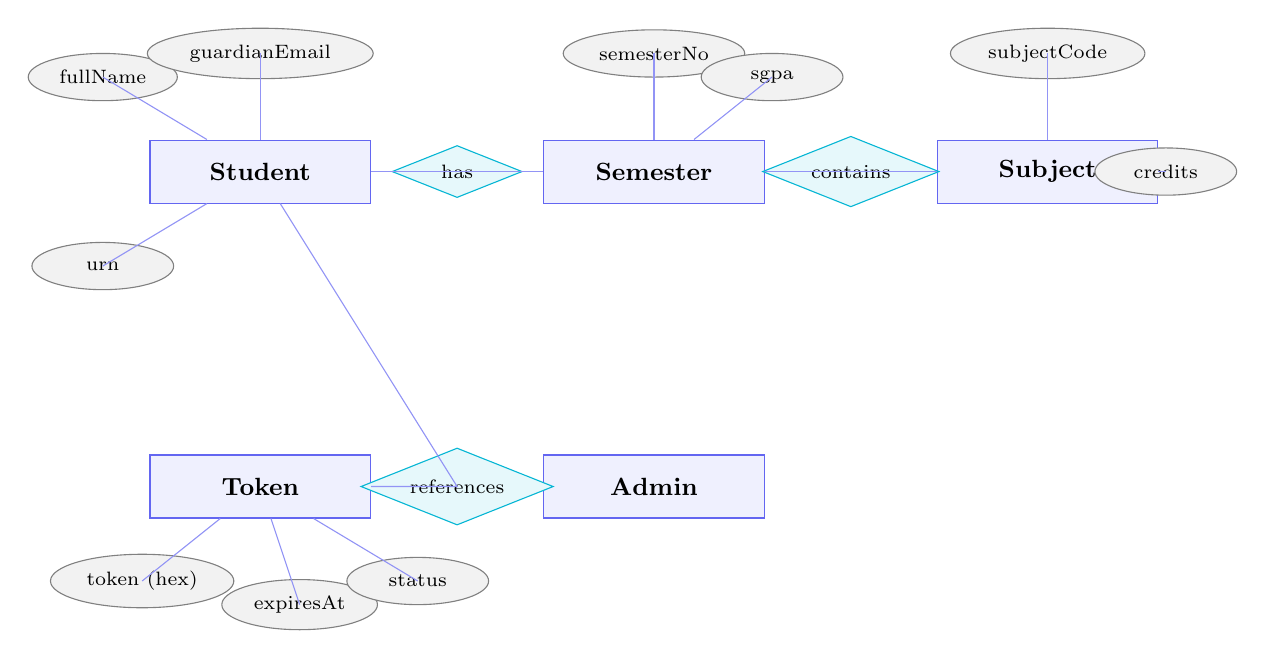
\begin{tikzpicture}[
  ent/.style={rectangle,draw=primaryblue,fill=primaryblue!10,minimum width=2.8cm,minimum height=0.8cm,align=center,font=\small\bfseries},
  rel/.style={diamond,draw=accentcyan,fill=accentcyan!10,aspect=2.5,font=\scriptsize},
  attr/.style={ellipse,draw=gray,fill=gray!10,minimum width=1.8cm,minimum height=0.6cm,align=center,font=\scriptsize},
  arr/.style={draw=primaryblue!70}
]
\node[ent] (student) at (0,0) {Student};
\node[ent] (semester) at (5,0) {Semester};
\node[ent] (subject) at (10,0) {Subject};
\node[ent] (token) at (0,-4) {Token};
\node[ent] (admin) at (5,-4) {Admin};

\node[rel] at (2.5,0) {has};
\node[rel] at (7.5,0) {contains};
\node[rel] at (2.5,-4) {references};

\draw[arr] (student)--(2.5,0)--(semester);
\draw[arr] (semester)--(7.5,0)--(subject);
\draw[arr] (token)--(2.5,-4)--(student);

\node[attr] at (-2,1.2) {fullName}; \draw[arr] (-2,1.2)--(student);
\node[attr] at (-2,-1.2) {urn}; \draw[arr] (-2,-1.2)--(student);
\node[attr] at (0,1.5) {guardianEmail}; \draw[arr] (0,1.5)--(student);

\node[attr] at (5,1.5) {semesterNo}; \draw[arr] (5,1.5)--(semester);
\node[attr] at (6.5,1.2) {sgpa}; \draw[arr] (6.5,1.2)--(semester);

\node[attr] at (10,1.5) {subjectCode}; \draw[arr] (10,1.5)--(subject);
\node[attr] at (11.5,0) {credits}; \draw[arr] (11.5,0)--(subject);

\node[attr] at (-1.5,-5.2) {token (hex)}; \draw[arr] (-1.5,-5.2)--(token);
\node[attr] at (0.5,-5.5) {expiresAt}; \draw[arr] (0.5,-5.5)--(token);
\node[attr] at (2,-5.2) {status}; \draw[arr] (2,-5.2)--(token);
\end{tikzpicture}
\caption{Entity-Relationship (ER) Diagram}
\end{figure}

\section{Database Design}

\subsection{Student Collection}
\begin{table}[H]
\centering
\caption{Student Collection Schema}
\renewcommand{\arraystretch}{1.3}
\begin{tabular}{|l|l|p{7cm}|}
\hline
\textbf{Field} & \textbf{Type} & \textbf{Description / Constraints}\\
\hline
fullName & String & Required, trimmed\\
\hline
urn & Number & University Roll Number, unique, required\\
\hline
crn & Number & College Roll Number, required\\
\hline
course & String & Validated against courseBranchMap\\
\hline
branch & String & Validated against course-specific branches\\
\hline
admissionYear & Number & Required, minimum 2000\\
\hline
graduationYear & Number & Required, must exceed admissionYear\\
\hline
guardianEmail & String & Required, only @gmail.com addresses\\
\hline
semesters & Array & Array of Semester sub-documents\\
\hline
cgpa & Number & Auto-calculated on save, 0-10\\
\hline
\end{tabular}
\end{table}

\subsection{Subject Collection}
\begin{table}[H]
\centering
\caption{Subject Collection Schema}
\renewcommand{\arraystretch}{1.3}
\begin{tabular}{|l|l|p{7cm}|}
\hline
\textbf{Field} & \textbf{Type} & \textbf{Description / Constraints}\\
\hline
subjectTitle & String & Required, trimmed\\
\hline
subjectCode & String & Required, unique, stored uppercase\\
\hline
type & String & `T' (Theory) or `P' (Practical)\\
\hline
credits & Number & Non-negative\\
\hline
maxInternalMarks & Number & Required\\
\hline
maxExternalMarks & Number & Required\\
\hline
maxTotalMarks & Number & Required; validated $\geq$ internal+external\\
\hline
minInternalPassMarks & Number & Required\\
\hline
minExternalPassMarks & Number & Required\\
\hline
minTotalPassMarks & Number & Required; validated $\leq$ maxTotalMarks\\
\hline
\end{tabular}
\end{table}

\subsection{Token Collection}
\begin{table}[H]
\centering
\caption{Token Collection Schema}
\renewcommand{\arraystretch}{1.3}
\begin{tabular}{|l|l|p{7cm}|}
\hline
\textbf{Field} & \textbf{Type} & \textbf{Description / Constraints}\\
\hline
token & String & 32-char hex string, unique, auto-generated\\
\hline
student & ObjectId & Reference to Student document\\
\hline
semester & Number & Semester number for which token was generated\\
\hline
sentVia & String & Email / SMS / Both\\
\hline
status & String & Active / Used / Expired\\
\hline
expiresAt & Date & Configured expiry timestamp\\
\hline
usedAt & Date & Timestamp of first access by guardian\\
\hline
\end{tabular}
\end{table}

\subsection{Admin Collection}
\begin{table}[H]
\centering
\caption{Admin Collection Schema}
\renewcommand{\arraystretch}{1.3}
\begin{tabular}{|l|l|p{7cm}|}
\hline
\textbf{Field} & \textbf{Type} & \textbf{Description / Constraints}\\
\hline
userName & String & 3-20 chars, unique, required\\
\hline
email & String & Unique, @gmail.com only, lowercase\\
\hline
password & String & bcrypt hashed (salt rounds: 12), min 8 chars\\
\hline
role & String & Enum: `admin'\\
\hline
\end{tabular}
\end{table}

\section{User Interface Design}
The Admin interface follows a dark-theme dashboard design with a fixed left sidebar for navigation. Key design decisions include:
\begin{itemize}
  \item \textbf{Sidebar Navigation:} Persistent sidebar with icons and labels for Dashboard, Upload Data, Students, Notifications, and Token Management.
  \item \textbf{Stat Cards:} The Dashboard displays summary statistics (total students, detained count, notifications sent, active tokens) as prominent card components.
  \item \textbf{Responsive Tables:} Student list and token list are displayed in responsive tables with search, filter, and pagination support.
  \item \textbf{Drag-and-Drop Upload:} The Upload Data page uses a drag-and-drop zone for file selection with real-time file type validation.
  \item \textbf{Data Preview:} A scrollable preview table shows parsed records before final submission.
  \item \textbf{Notification Form:} A two-panel layout with student selection (with search and filters) on the left and notification configuration (expiry, semester selection) on the right.
\end{itemize}

The Guardian Portal uses a clean, light-themed layout with the following sections:
\begin{itemize}
  \item Student profile card (name, URN, course, branch).
  \item SGPA trend line chart (Recharts \texttt{LineChart}).
  \item Semester accordion panels: each panel expands to show a table of subject marks.
  \item Attendance ring indicator (circle progress component).
  \item Detention alert banner (conditionally rendered).
\end{itemize}

\section{Methodology}
The development methodology was component-driven on the frontend and route-controller-model on the backend:

\textbf{Frontend Methodology:}
\begin{itemize}
  \item All UI is built as reusable React components.
  \item State management uses React Context API for global authentication state.
  \item API calls are centralised in an Axios instance configured with base URL and credentials.
  \item Protected routes use a \texttt{ProtectedRoute} wrapper component that checks authentication state before rendering admin pages.
\end{itemize}

\textbf{Backend Methodology:}
\begin{itemize}
  \item Routes are separated by resource (auth, student, mailsender, token, report).
  \item Controllers handle business logic, decoupled from route definitions.
  \item All asynchronous controller functions are wrapped in an \texttt{asyncHandler} utility to avoid repetitive try-catch blocks.
  \item Consistent JSON responses are returned via \texttt{ApiResponse} and \texttt{ApiError} utility classes.
  \item Session middleware validates admin sessions on all protected routes via an \texttt{isAuthenticated} middleware.
\end{itemize}

\chapter{Implementation and Testing}

\section{Introduction to Languages, IDEs, Tools and Technologies}

\subsection{JavaScript / ES2022+}
JavaScript is the primary programming language used for both the frontend and backend of ASTNS. Modern ES2022+ features used in the project include: arrow functions, async/await, destructuring assignment, optional chaining (\texttt{?.}), nullish coalescing (\texttt{??}), template literals, and ES modules (\texttt{import}/\texttt{export}).

\subsection{React 19}
React is an open-source JavaScript library for building user interfaces. ASTNS uses React 19, which introduces improved concurrent rendering and server-side rendering support. Key React concepts used in the project:
\begin{itemize}
  \item \textbf{Functional Components:} All UI components are written as functions using hooks.
  \item \textbf{useState / useEffect:} For local state management and side-effect handling.
  \item \textbf{useContext:} For global authentication state via \texttt{AuthContext}.
  \item \textbf{React Router DOM v7:} For client-side routing between Admin pages and Guardian Portal.
  \item \textbf{React Hook Form v7:} For form state management and validation.
\end{itemize}

\subsection{Vite 7}
Vite is a fast build tool for frontend development. It provides hot module replacement (HMR) during development and optimised production builds. ASTNS uses Vite for its near-instant dev server startup and efficient bundling.

\subsection{Tailwind CSS 4}
Tailwind CSS is a utility-first CSS framework. Instead of pre-built components, Tailwind provides low-level utility classes that allow developers to build custom designs directly in HTML/JSX markup. ASTNS uses Tailwind for all layout, typography, colour, and responsive design.

\subsection{Node.js v20 LTS}
Node.js is the JavaScript runtime environment used to run the backend server. ASTNS uses Node.js v20 (Long-Term Support), which provides improved performance through the V8 engine v11.3.

\subsection{Express.js 5}
Express.js is a minimal, un-opinionated web framework for Node.js. ASTNS uses Express.js v5, which introduces improved error handling (async errors are now automatically forwarded to error middleware without explicit \texttt{next(err)} calls).

Key Express.js features used:
\begin{itemize}
  \item Middleware pipeline (body parser, cookie parser, CORS, session validation).
  \item Router-based route modularisation.
  \item Error handling middleware for consistent API error responses.
\end{itemize}

\subsection{MongoDB Atlas + Mongoose 9}
MongoDB Atlas is the cloud-hosted deployment of MongoDB, a document-oriented NoSQL database. ASTNS uses the M0 free tier cluster. Mongoose provides schema-based modelling for MongoDB documents, with built-in validation, middleware hooks, and population (joins via references).

Key Mongoose features used in ASTNS:
\begin{itemize}
  \item \texttt{pre('validate')} hook: Used in \texttt{SubjectPerformance} schema to auto-calculate \texttt{totalMarks} and set \texttt{status} (Pass/Detained) before validation.
  \item \texttt{pre('save')} hook: Used in \texttt{Student} schema to auto-calculate \texttt{cgpa} from all semester SGPAs.
  \item \texttt{populate()}: Used in student and token controllers to resolve ObjectId references into full documents.
  \item \texttt{aggregate()}: Used in the dashboard stats controller for branch distribution and average CGPA calculations.
\end{itemize}

\subsection{Nodemailer 8}
Nodemailer is a Node.js module for sending emails. ASTNS uses Nodemailer with Gmail SMTP (port 465, SSL) to dispatch HTML-formatted notification emails. The email template includes the student's name, the guardian's name, and a styled ``View Report'' button containing the token URL.

\subsection{Vercel}
Vercel is a cloud platform for frontend frameworks and serverless functions. ASTNS deploys:
\begin{itemize}
  \item The React SPA as a static site served from Vercel's global CDN.
  \item The Express.js backend as Vercel serverless functions (via \texttt{vercel.json} routing configuration).
\end{itemize}

\subsection{Git and GitHub}
Git was used for version control throughout the project. The repository is hosted on GitHub with three contributors (one per team member). Feature branches were used for each major module, with pull requests and code review before merging into the main branch.

\subsection{Visual Studio Code}
VS Code was the primary IDE used by the team. Extensions used include: ESLint, Prettier, Tailwind CSS IntelliSense, MongoDB for VS Code, REST Client, GitLens.

\subsection{Postman}
Postman was used for API testing during backend development. Collections were created for each resource group (Auth, Students, Tokens, Notifications, Report).

\section{Algorithm / Pseudocode}

\subsection{Token Generation and Email Dispatch Algorithm}

\begin{verbatim}
ALGORITHM SendNotifications(recipients, semester, expiry):
  INPUT: recipients = [{studentId, email}], semester, expiry duration
  OUTPUT: {success_count, failure_count, details}

  hours = EXPIRY_MAP[expiry]  // 24, 48, 72, or 168
  expiresAt = CURRENT_TIME + hours * 3600 * 1000

  FOR EACH recipient IN recipients DO PARALLEL:
    student = FIND_STUDENT_BY_ID(recipient.studentId)
    IF student NOT FOUND:
      RECORD failure for recipient
      CONTINUE

    token_string = CRYPTO.RANDOM_BYTES(16).TO_HEX()
    token_doc = CREATE_TOKEN({
      student: student._id,
      token: token_string,
      semester: semester,
      expiresAt: expiresAt,
      status: "Active"
    })

    guardian_url = FRONTEND_URL + "/guardian?token=" + token_string
    email_sent = SEND_EMAIL(recipient.email, student.fullName, guardian_url)

    IF email_sent:
      RECORD success for student
    ELSE:
      RECORD failure for student

  RETURN {success_count, failure_count, details}
END ALGORITHM
\end{verbatim}

\subsection{Token Validation Algorithm}

\begin{verbatim}
ALGORITHM ValidateToken(token_string):
  INPUT: token_string (32-char hex from URL query parameter)
  OUTPUT: student academic data OR error response

  // Step 1: Auto-expire stale tokens
  UPDATE ALL TOKENS WHERE status="Active" AND expiresAt < NOW()
    SET status = "Expired"

  // Step 2: Find token
  token_doc = FIND_TOKEN({token: token_string})
    WITH POPULATE student -> semesters -> subjects -> subject_details

  IF token_doc NOT FOUND:
    RETURN HTTP 404 "Invalid or unknown token"

  IF token_doc.status == "Expired":
    RETURN HTTP 410 "This token has expired"

  // Step 3: Mark as used on first access
  IF token_doc.status == "Active":
    UPDATE token_doc SET status="Used", usedAt=NOW()

  RETURN HTTP 200 WITH student_data
END ALGORITHM
\end{verbatim}

\subsection{CGPA Auto-Calculation}

\begin{verbatim}
HOOK Student.pre("save"):
  IF semesters IS EMPTY:
    SET cgpa = 0
    RETURN

  total_sgpa = SUM(semester.sgpa FOR ALL semester IN semesters)
  cgpa = ROUND(total_sgpa / COUNT(semesters), 2)
  SET this.cgpa = cgpa
END HOOK
\end{verbatim}

\section{Testing Techniques}
ASTNS was tested using a combination of the following techniques:

\begin{itemize}
  \item \textbf{Unit Testing:} Individual Mongoose schema validators were tested by attempting to save documents with invalid data (e.g., marks exceeding maximum, invalid course-branch combinations, invalid email formats) and verifying that validation errors were thrown correctly.
  \item \textbf{API Integration Testing:} All REST API endpoints were tested using Postman. Each endpoint was tested for: correct response status codes, correct response body structure, error handling for missing/invalid inputs, and authentication enforcement on protected routes.
  \item \textbf{Functional Testing:} The complete user workflows (Admin login, CSV upload, notification dispatch, Guardian Portal access) were tested manually end-to-end.
  \item \textbf{Boundary Testing:} Edge cases such as empty CSV files, CSVs with missing columns, tokens accessed after expiry, and concurrent notification dispatch to large student batches were tested.
  \item \textbf{Cross-Browser Testing:} The Admin Dashboard and Guardian Portal were tested on Google Chrome (v124), Mozilla Firefox (v125), and Microsoft Edge (v124) on Windows; and on Safari on iOS.
  \item \textbf{Responsive Design Testing:} The Guardian Portal was tested on viewport widths of 375px (mobile), 768px (tablet), and 1440px (desktop) using Chrome DevTools.
\end{itemize}

\section{Test Cases}

\begin{table}[H]
\centering
\caption{Test Cases -- Authentication Module}
\renewcommand{\arraystretch}{1.3}
\begin{tabular}{|p{0.8cm}|p{3cm}|p{4cm}|p{4.5cm}|}
\hline
\textbf{TC\#} & \textbf{Test Case} & \textbf{Input / Steps} & \textbf{Expected Result}\\
\hline
TC1 & Admin Login -- Valid & Email: admin@gmail.com, Password: correct & HTTP 200, session cookie set, redirect to Dashboard\\
\hline
TC2 & Admin Login -- Wrong Password & Email: admin@gmail.com, Password: wrong & HTTP 401 ``Invalid credentials''\\
\hline
TC3 & Admin Login -- Unknown Email & Email: unknown@gmail.com & HTTP 404 ``Admin not found''\\
\hline
TC4 & Admin Logout & Click Logout button & Session deleted, cookie cleared, redirect to Login\\
\hline
TC5 & Access Protected Route Without Session & Navigate to /admin/dashboard without login & HTTP 401, redirect to Login page\\
\hline
\end{tabular}
\end{table}

\begin{table}[H]
\centering
\caption{Test Cases -- Data Upload Module}
\renewcommand{\arraystretch}{1.3}
\begin{tabular}{|p{0.8cm}|p{3cm}|p{4cm}|p{4.5cm}|}
\hline
\textbf{TC\#} & \textbf{Test Case} & \textbf{Input / Steps} & \textbf{Expected Result}\\
\hline
TC6 & Upload Valid CSV & Upload correctly formatted CSV & Records parsed, preview table displayed correctly\\
\hline
TC7 & Upload CSV with Missing Columns & CSV missing ``guardianEmail'' column & Validation error shown, no records saved\\
\hline
TC8 & Upload CSV with Invalid Marks & Student marks > maxTotalMarks & Mongoose validation error returned, record rejected\\
\hline
TC9 & Upload CSV with Invalid Course & Course not in courseBranchMap & Validation error: ``not a valid course''\\
\hline
TC10 & Upload Non-CSV File & Upload .txt file & Frontend rejects file, error message shown\\
\hline
\end{tabular}
\end{table}

\begin{table}[H]
\centering
\caption{Test Cases -- Notification Module}
\renewcommand{\arraystretch}{1.3}
\begin{tabular}{|p{0.8cm}|p{3cm}|p{4cm}|p{4.5cm}|}
\hline
\textbf{TC\#} & \textbf{Test Case} & \textbf{Input / Steps} & \textbf{Expected Result}\\
\hline
TC11 & Send Notification -- Single Student & Select 1 student, click Send & 1 token created, 1 email dispatched, success shown\\
\hline
TC12 & Send Notification -- Batch & Select 20 students, click Send & 20 tokens created, 20 emails dispatched in parallel\\
\hline
TC13 & Send Notification -- No Students Selected & Click Send with no selection & Frontend validation: ``Select at least one student''\\
\hline
TC14 & Email Content Verification & Inspect received email & Email contains student name, ``View Report'' button, correct token URL\\
\hline
\end{tabular}
\end{table}

\begin{table}[H]
\centering
\caption{Test Cases -- Guardian Portal}
\renewcommand{\arraystretch}{1.3}
\begin{tabular}{|p{0.8cm}|p{3cm}|p{4cm}|p{4.5cm}|}
\hline
\textbf{TC\#} & \textbf{Test Case} & \textbf{Input / Steps} & \textbf{Expected Result}\\
\hline
TC15 & Valid Token Access & Open URL with valid token & Guardian Portal renders student academic data\\
\hline
TC16 & Expired Token Access & Open URL with expired token & Access Denied page with expiry message\\
\hline
TC17 & Revoked Token Access & Admin revokes token; Guardian opens URL & Access Denied page with revocation message\\
\hline
TC18 & Invalid Token & Manually enter random token in URL & HTTP 404 ``Invalid or unknown token''\\
\hline
TC19 & SGPA Chart Rendering & Student has 4 semester records & Line chart displays 4 data points correctly\\
\hline
TC20 & Detention Flag Display & Student has a detained subject & Detention badge displayed on that subject row\\
\hline
\end{tabular}
\end{table}

\chapter{Results and Discussions}

\section{User Interface Representation}

\subsection{Brief Description of Various Modules}

\textbf{1. Login Module:} The Login page is the entry point for administrators. It displays a clean, centred card with email and password fields and a ``Sign In'' button. Client-side validation ensures both fields are filled before submission. On successful authentication, the admin is redirected to the Dashboard. On failure, an error message is shown.

\textbf{2. Admin Dashboard Module:} The Dashboard displays four summary stat cards: Total Students, Detained Students, Total Notifications Sent, and Active Tokens. Below the cards, a bar chart shows notification activity over the past 30 days. A branch distribution table shows the count of students per branch.

\textbf{3. Upload Data Module:} Administrators can drag-and-drop or browse to upload CSV or Excel files. After upload, the system parses the file and displays a paginated preview table showing all detected student records. The admin selects the target semester and clicks ``Submit'' to save the records to the database.

\textbf{4. Student List Module:} Displays a searchable, filterable table of all students. The admin can search by student name, URN, or CRN, and filter by course or branch. Each row shows the student's name, URN, course, branch, and current CGPA, with a link to the Student Detail page.

\textbf{5. Student Detail Module:} Shows the complete academic profile of a selected student. The page displays the student's personal information (name, URN, CRN, course, branch, admission year), an SGPA trend line chart, and an accordion of all semesters. Each semester accordion expands to show a table of subject marks (internal, external, total, max marks, status).

\textbf{6. Send Notification Module:} The left panel displays all students with checkboxes for selection. Search and filter controls help narrow the list. The right panel provides configuration: semester selection, token expiry, and a ``Send Notifications'' button. A progress indicator shows dispatch status for each student.

\textbf{7. Token Management Module:} Displays all generated tokens in a table with columns: student name, URN, semester, status (Active / Used / Expired), created date, expiry date, and a Revoke button for active tokens. Administrators can filter by status.

\textbf{8. Guardian Dashboard Module:} Accessed via the token URL. Shows the student's profile, SGPA line chart, attendance ring, and expandable semester panels with subject-wise marks. Detention alerts are shown as a prominent red banner if any detained subjects exist.

\textbf{9. Access Denied Module:} Shown when an invalid, expired, or revoked token is used. Displays an appropriate message explaining why access was denied.

\section{Snapshots of System with Details}

\subsection{Login Page}
\begin{figure}[H]
\centering
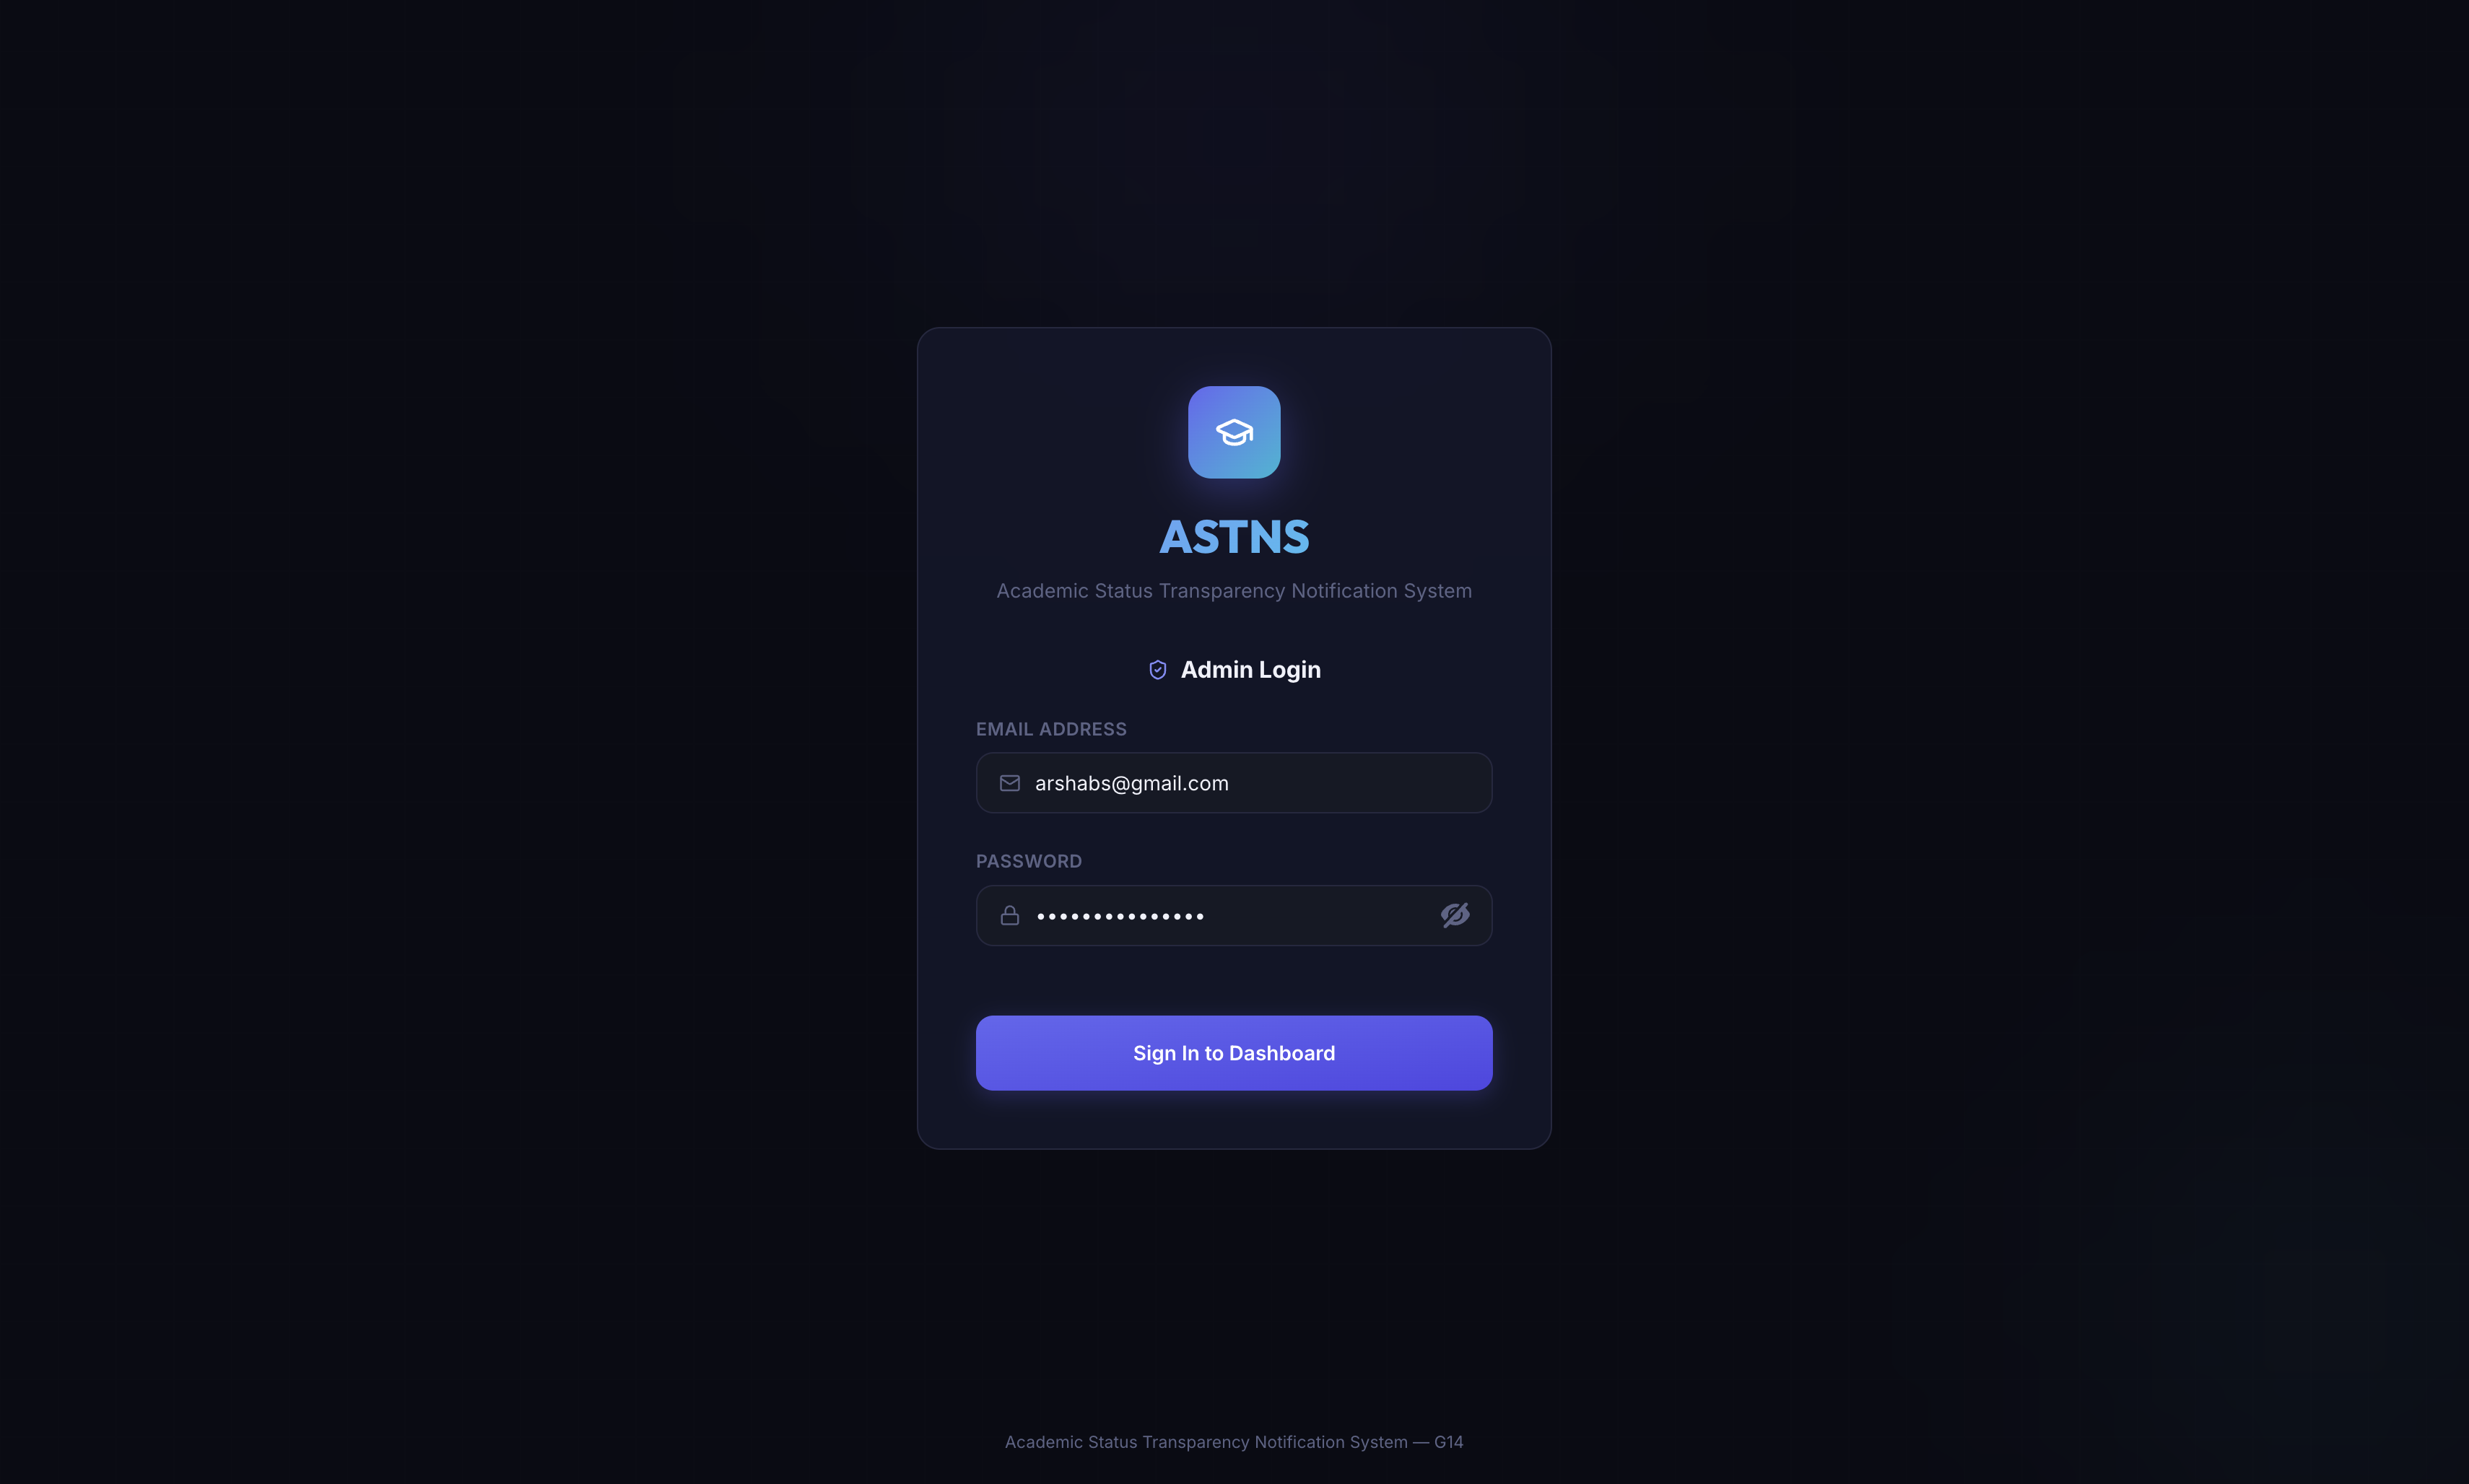
\includegraphics[width=0.85\textwidth]{assets/pic1.png}
\caption{Login Page -- Admin Authentication Interface}
\end{figure}
The Login page features a dark-themed card centred on the viewport. The form contains email and password inputs with client-side validation. On successful authentication, a session cookie is set and the admin is redirected to the Dashboard.

\subsection{Admin Dashboard}
\begin{figure}[H]
\centering
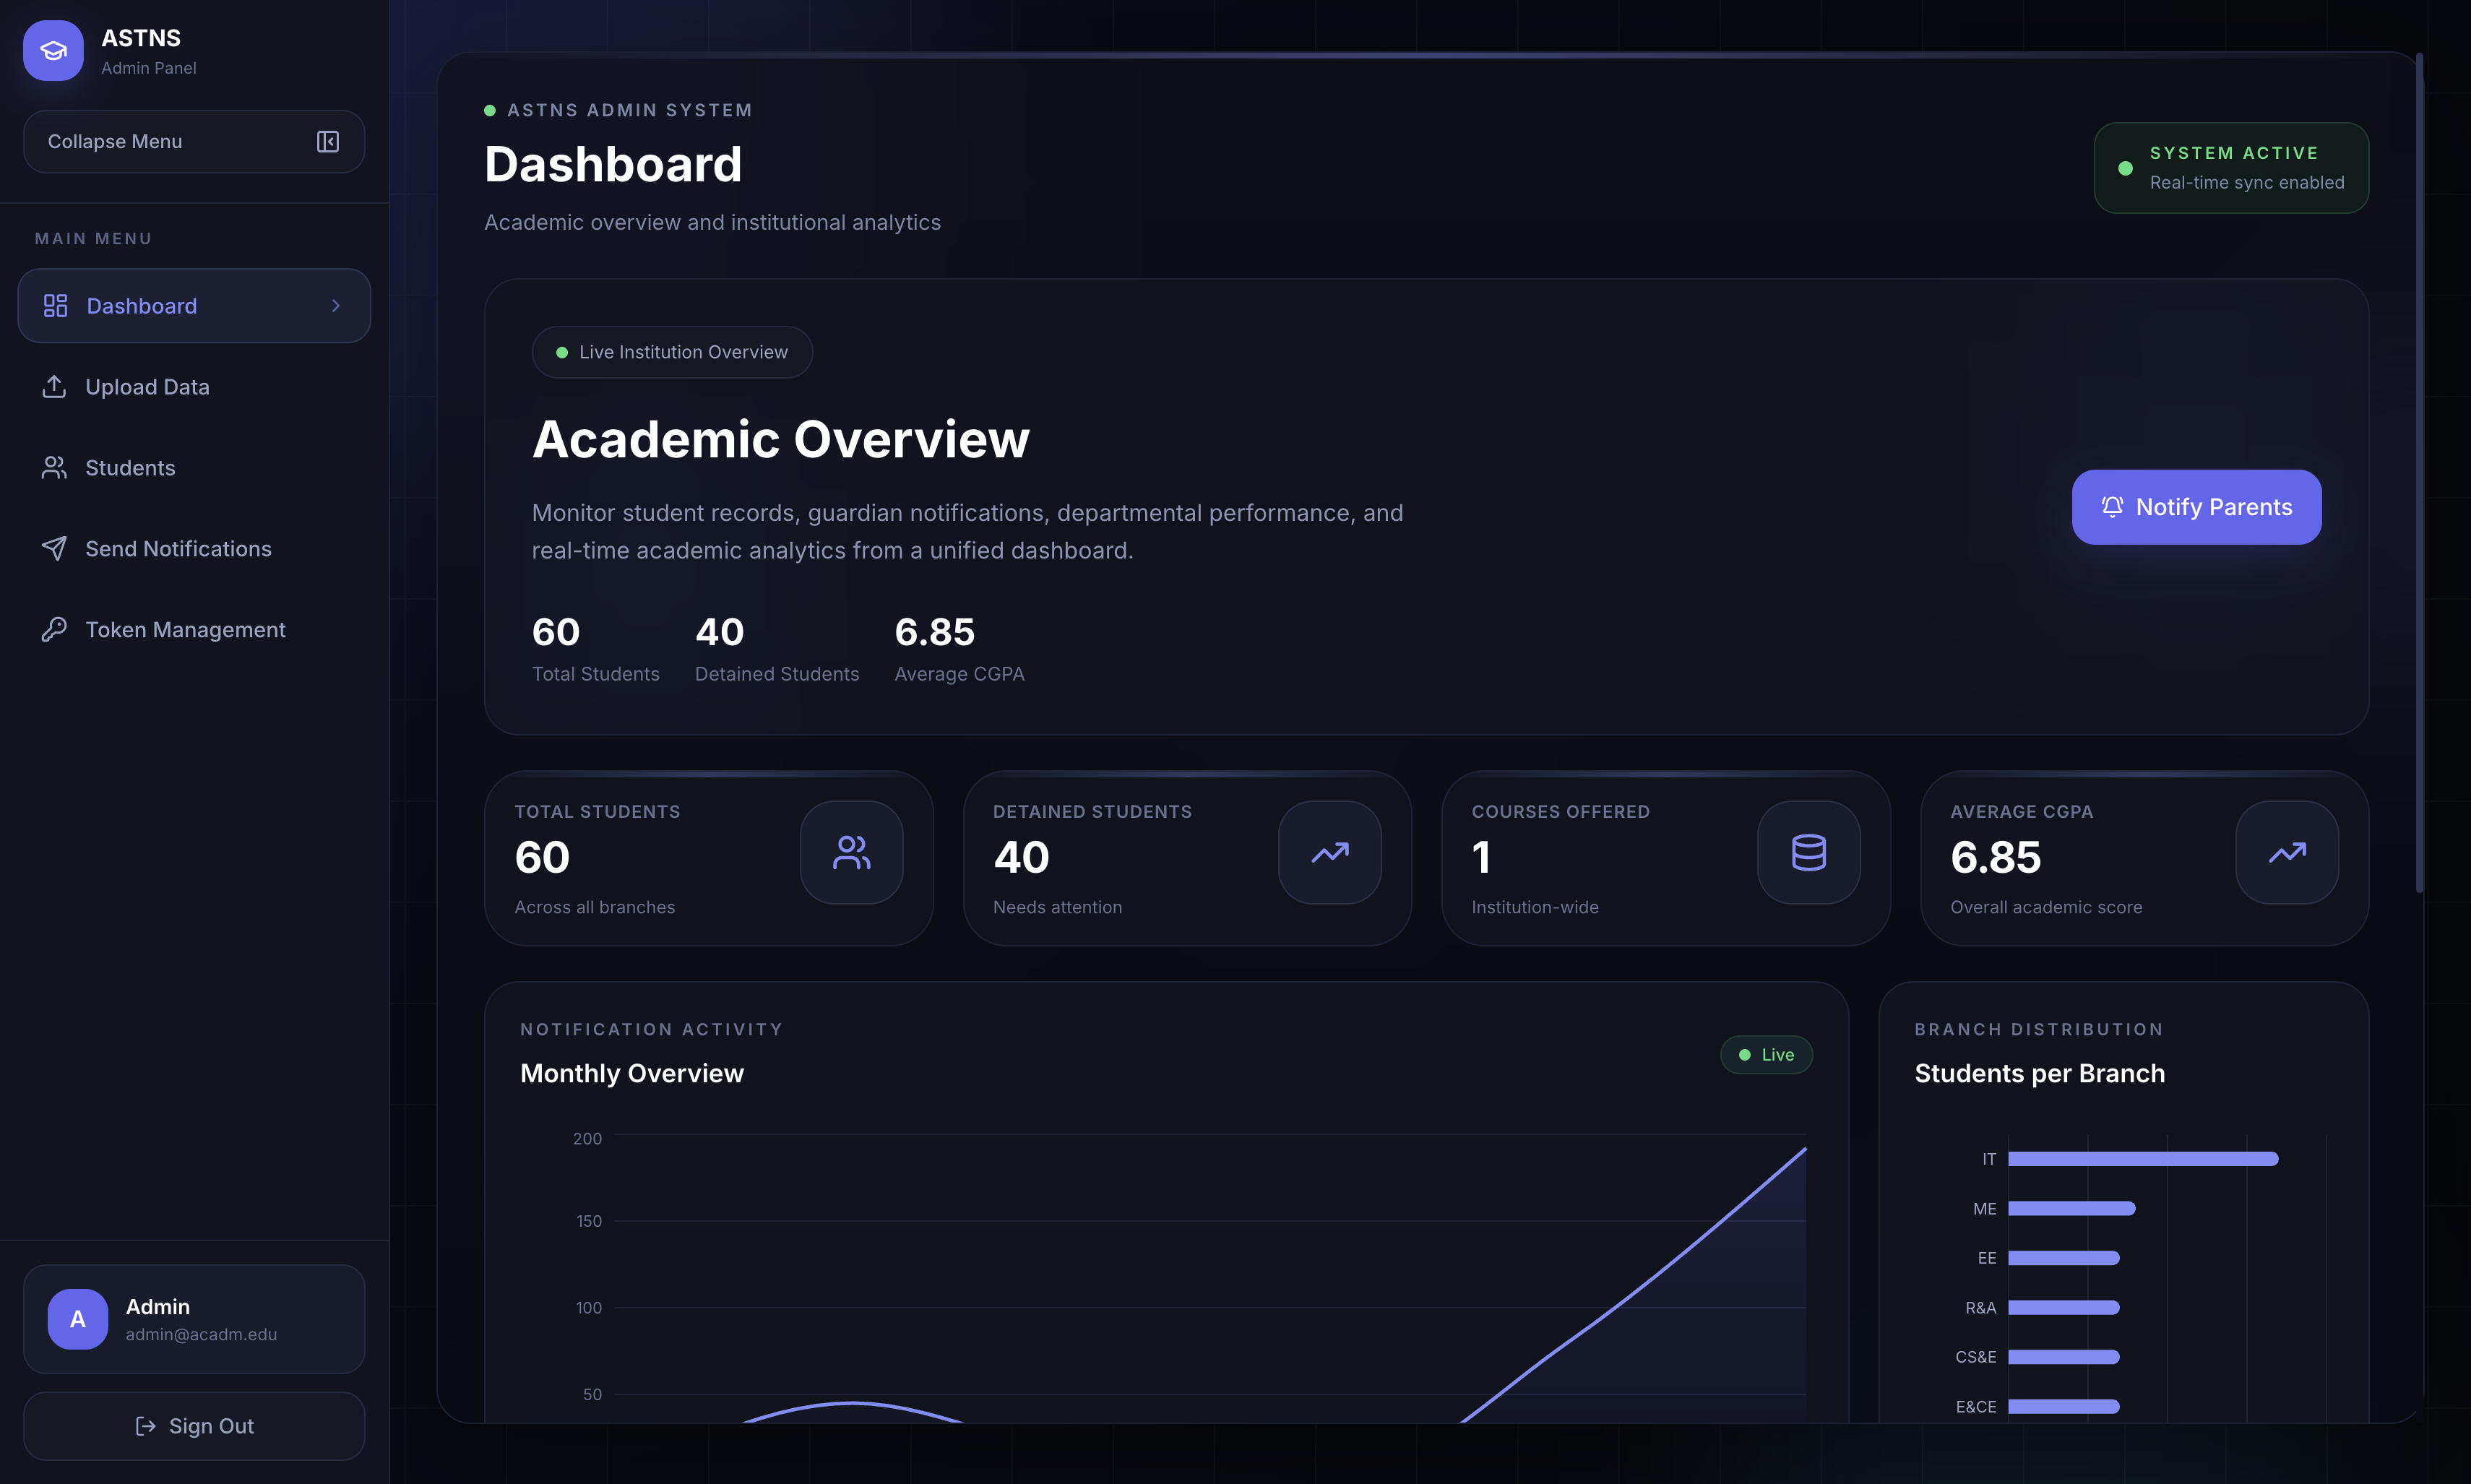
\includegraphics[width=0.85\textwidth]{assets/pic2.png}
\caption{Admin Dashboard -- Overview with Stats and Charts}
\end{figure}
The Dashboard presents four metric cards at the top: Total Students, Detained Count, Notifications Sent, and Active Tokens. A bar chart below shows notification activity. The sidebar remains visible on all Admin pages for easy navigation.

\subsection{Upload Data Page}
\begin{figure}[H]
\centering
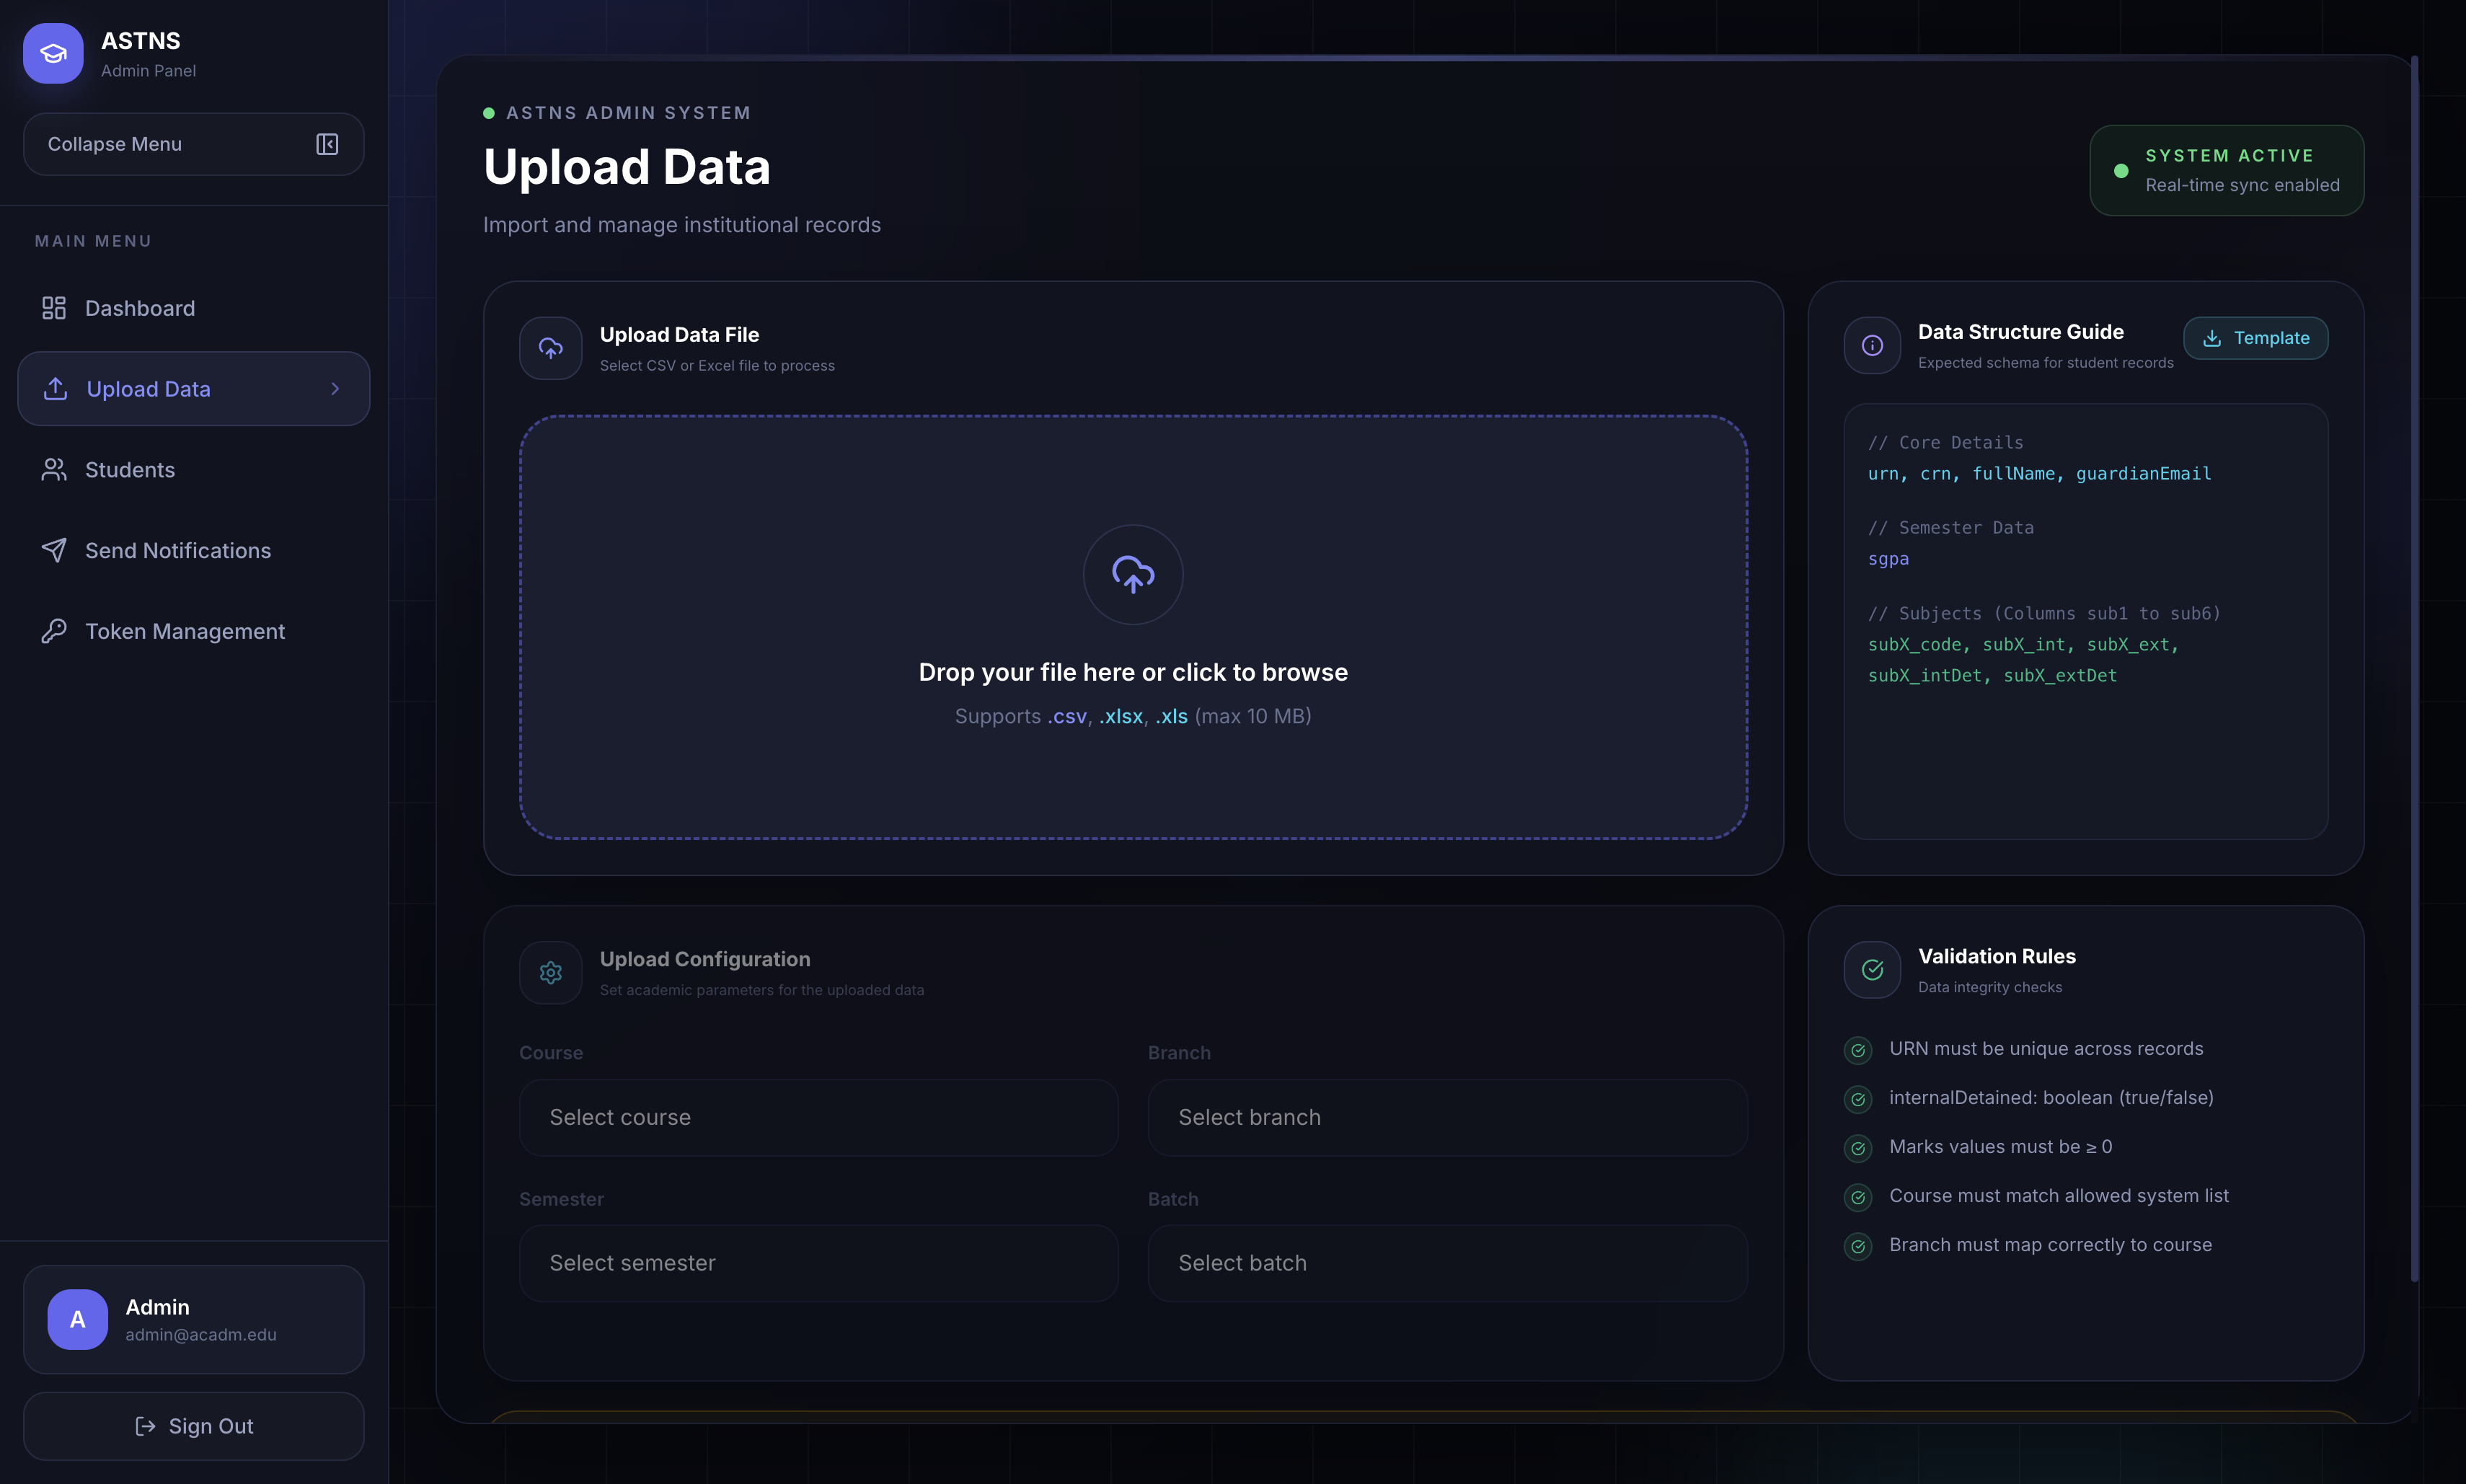
\includegraphics[width=0.85\textwidth]{assets/pic3.png}
\caption{Upload Data Page -- CSV Bulk Upload Interface}
\end{figure}
The Upload Data page features a drag-and-drop zone. After file selection, the system parses the file and renders a preview table. The admin selects the semester and confirms submission.

\subsection{Student List Page}
\begin{figure}[H]
\centering
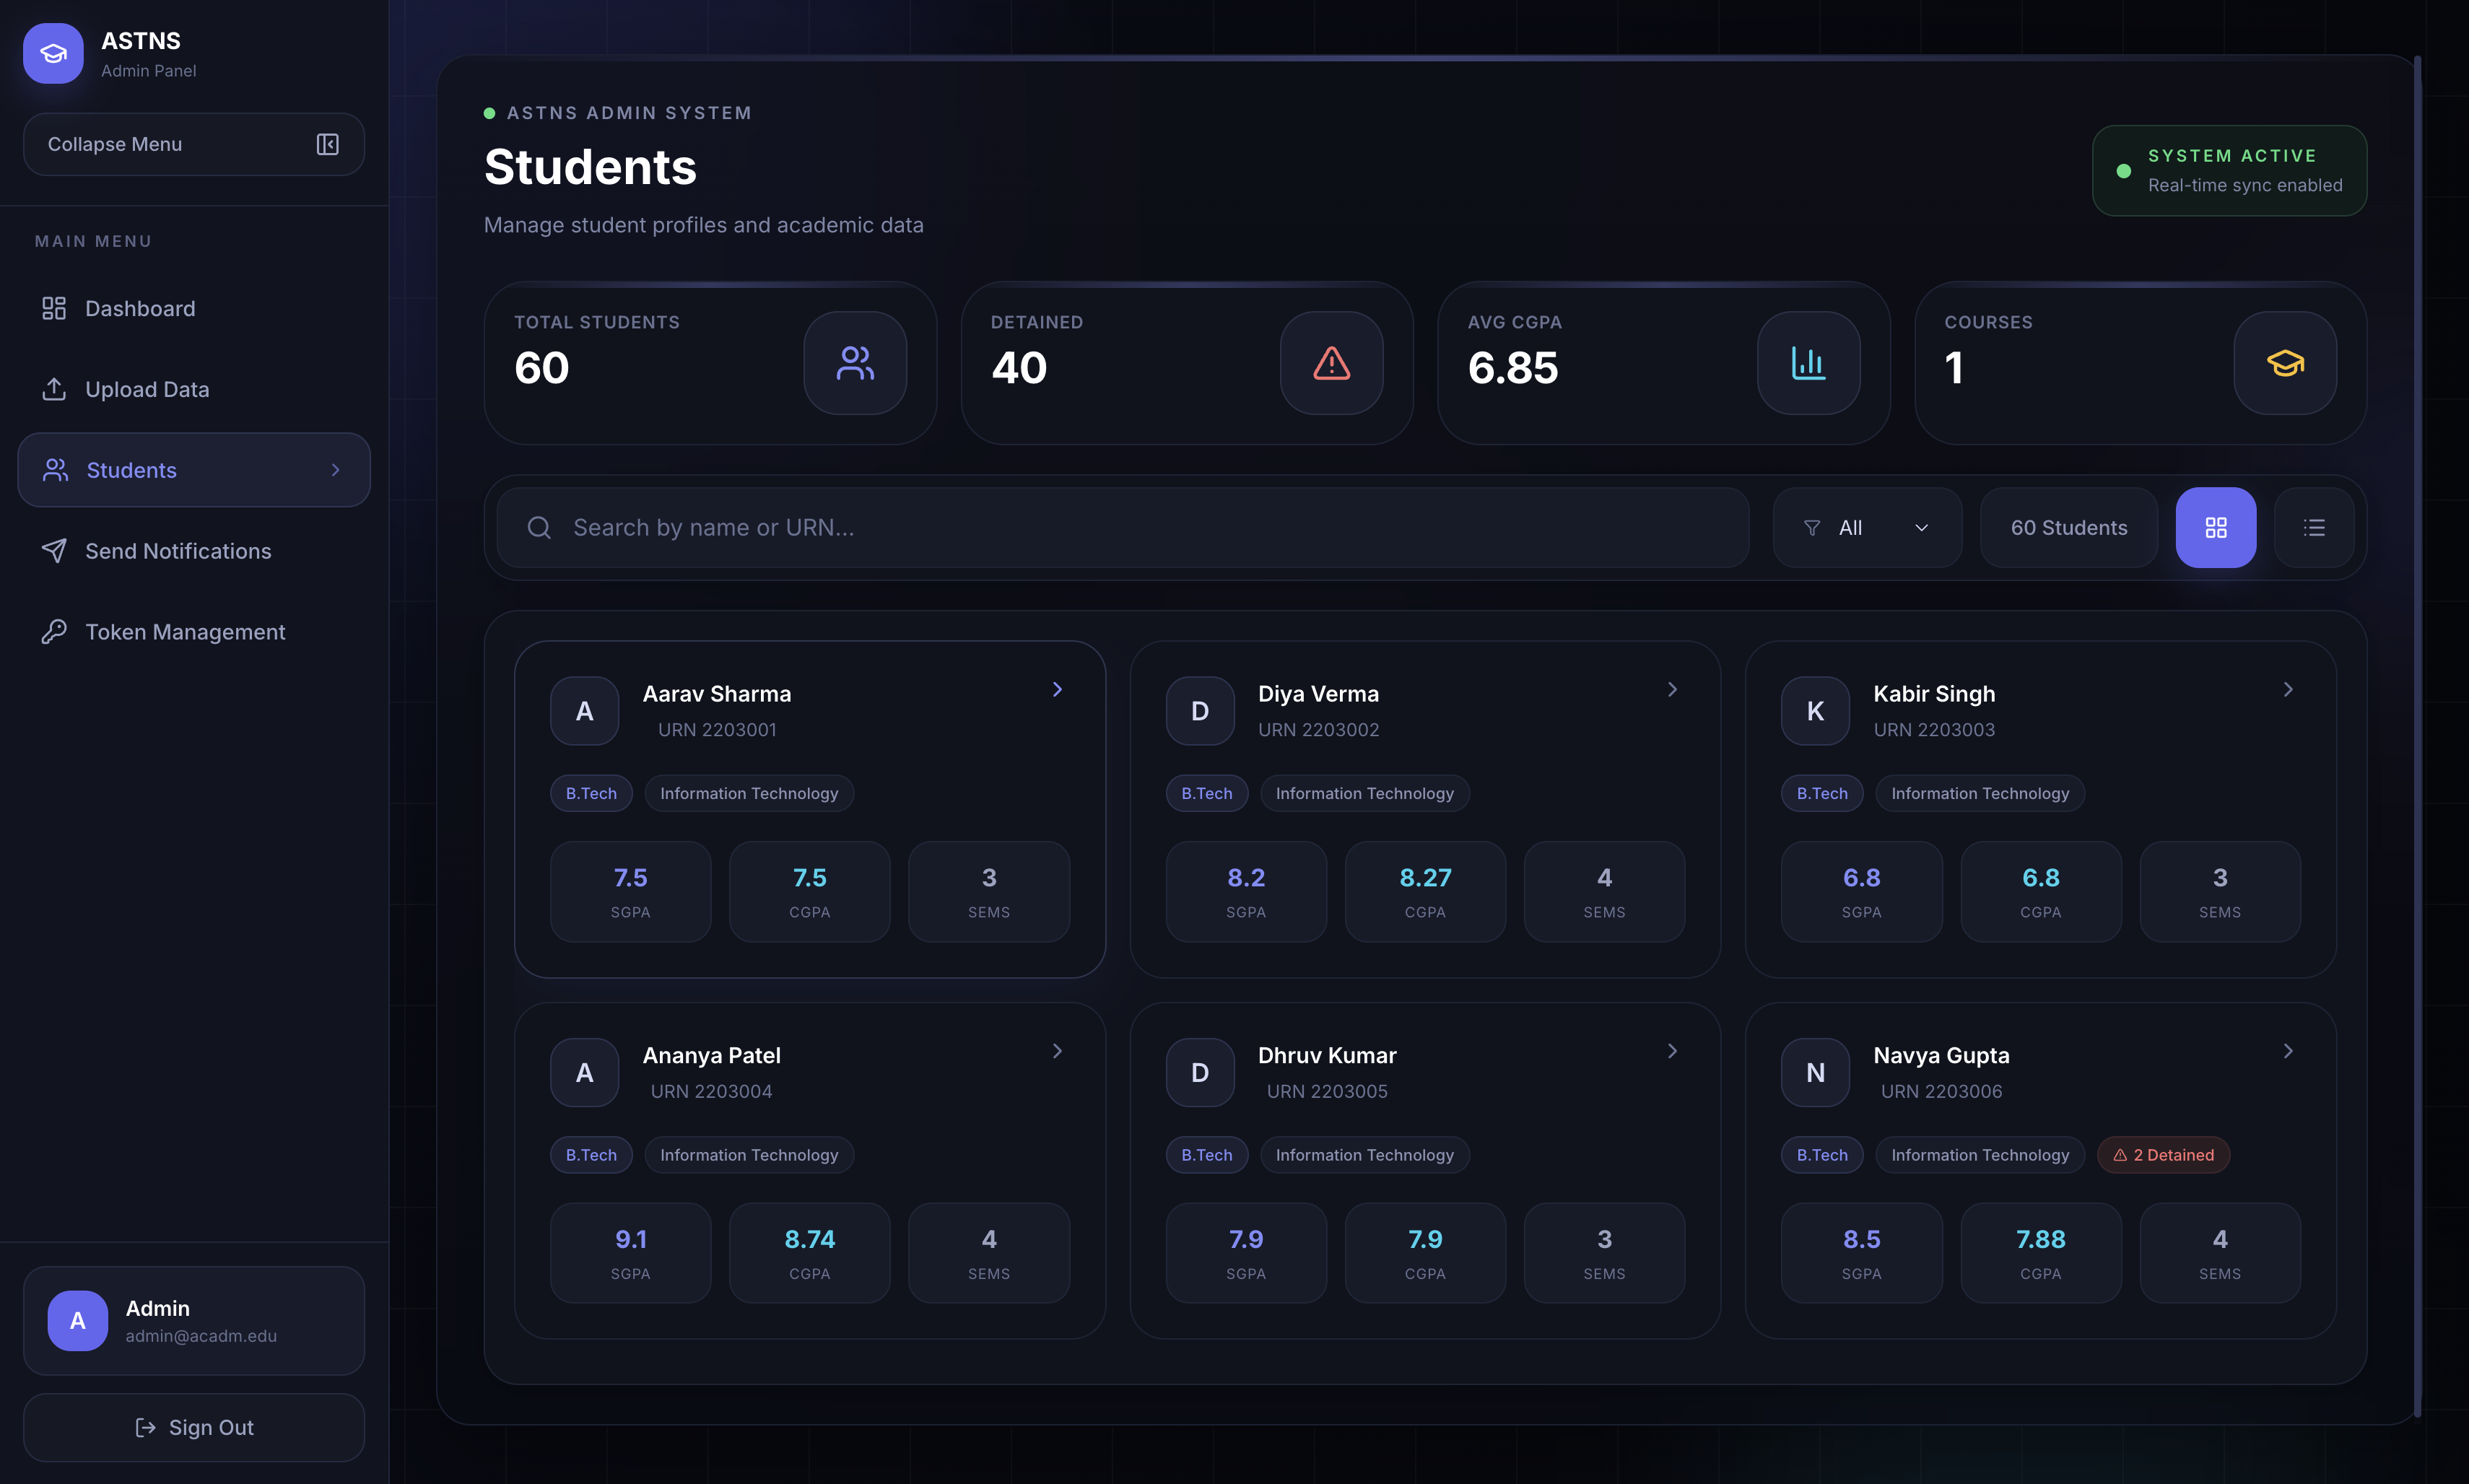
\includegraphics[width=0.85\textwidth]{assets/pic4.png}
\caption{Student List Page -- Searchable and Filterable Student Records}
\end{figure}
All students are displayed in a sortable table. The search bar filters by name, URN, or CRN. Dropdown filters allow selection by course and branch.

\subsection{Student Detail Page}
\begin{figure}[H]
\centering
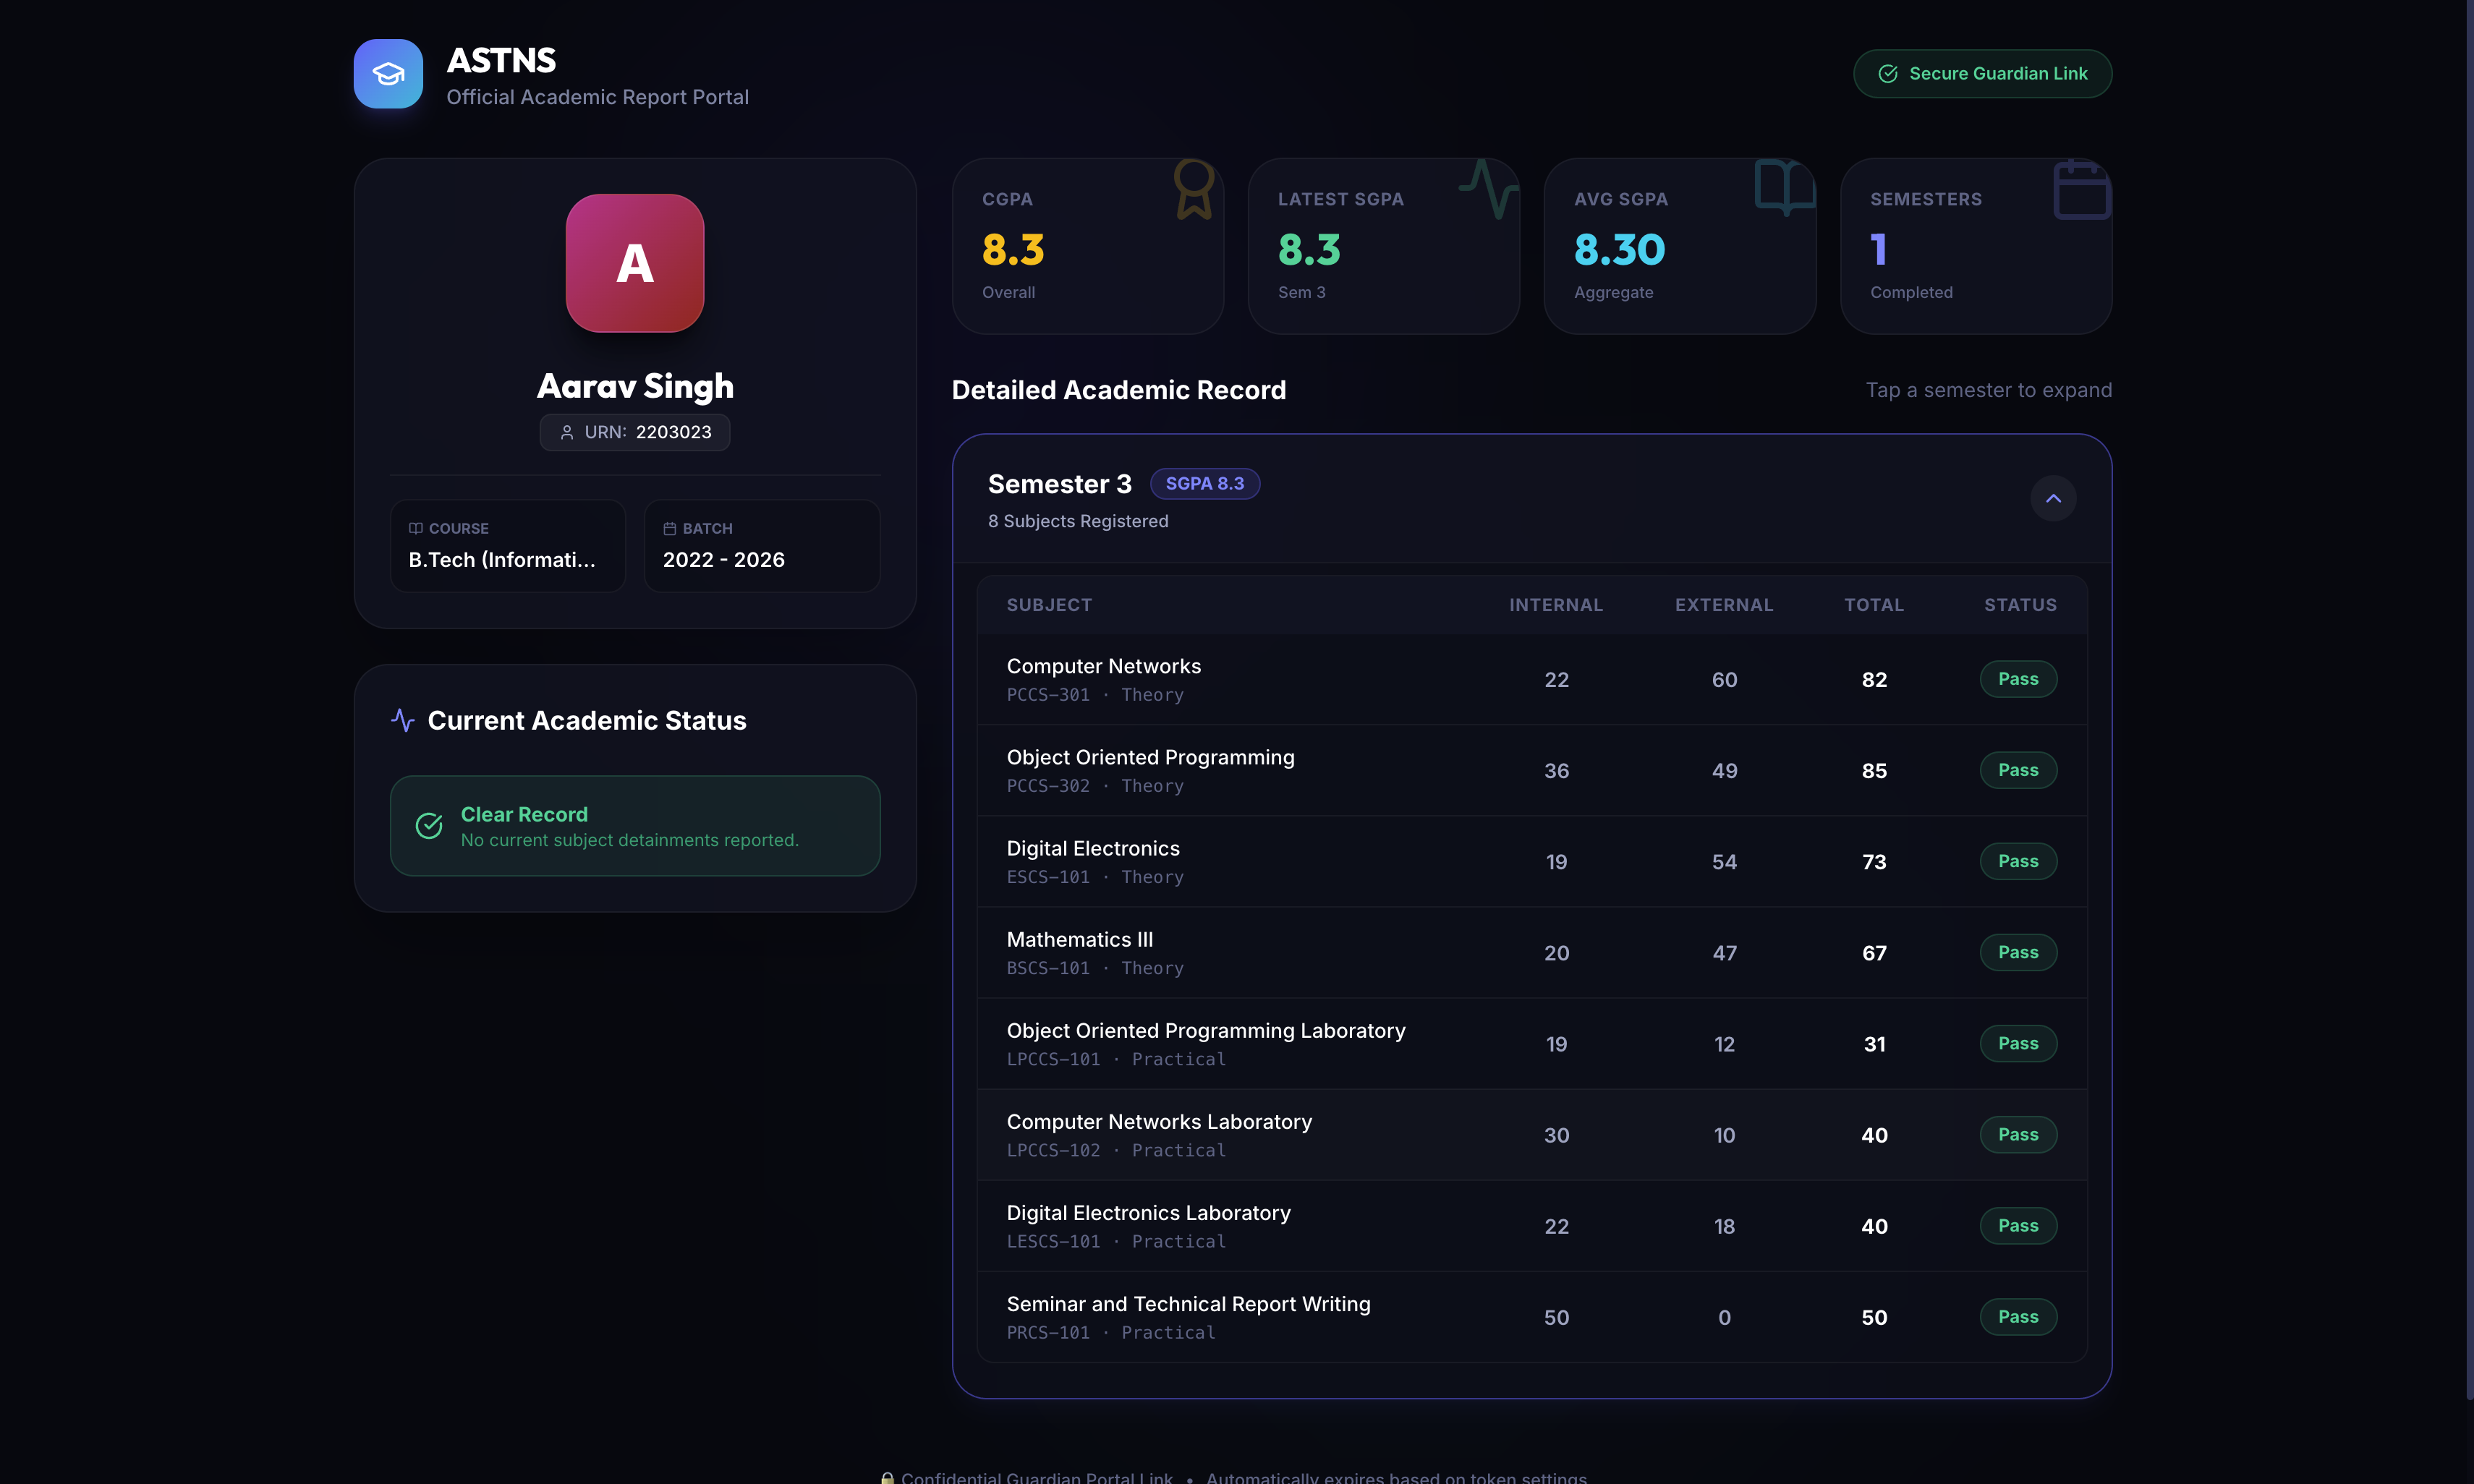
\includegraphics[width=0.85\textwidth]{assets/pic5.png}
\caption{Student Detail Page -- Individual Academic Profile}
\end{figure}
The Student Detail page shows the student's complete profile with an SGPA trend chart and expandable semester mark tables.

\subsection{Send Notification Page}
\begin{figure}[H]
\centering
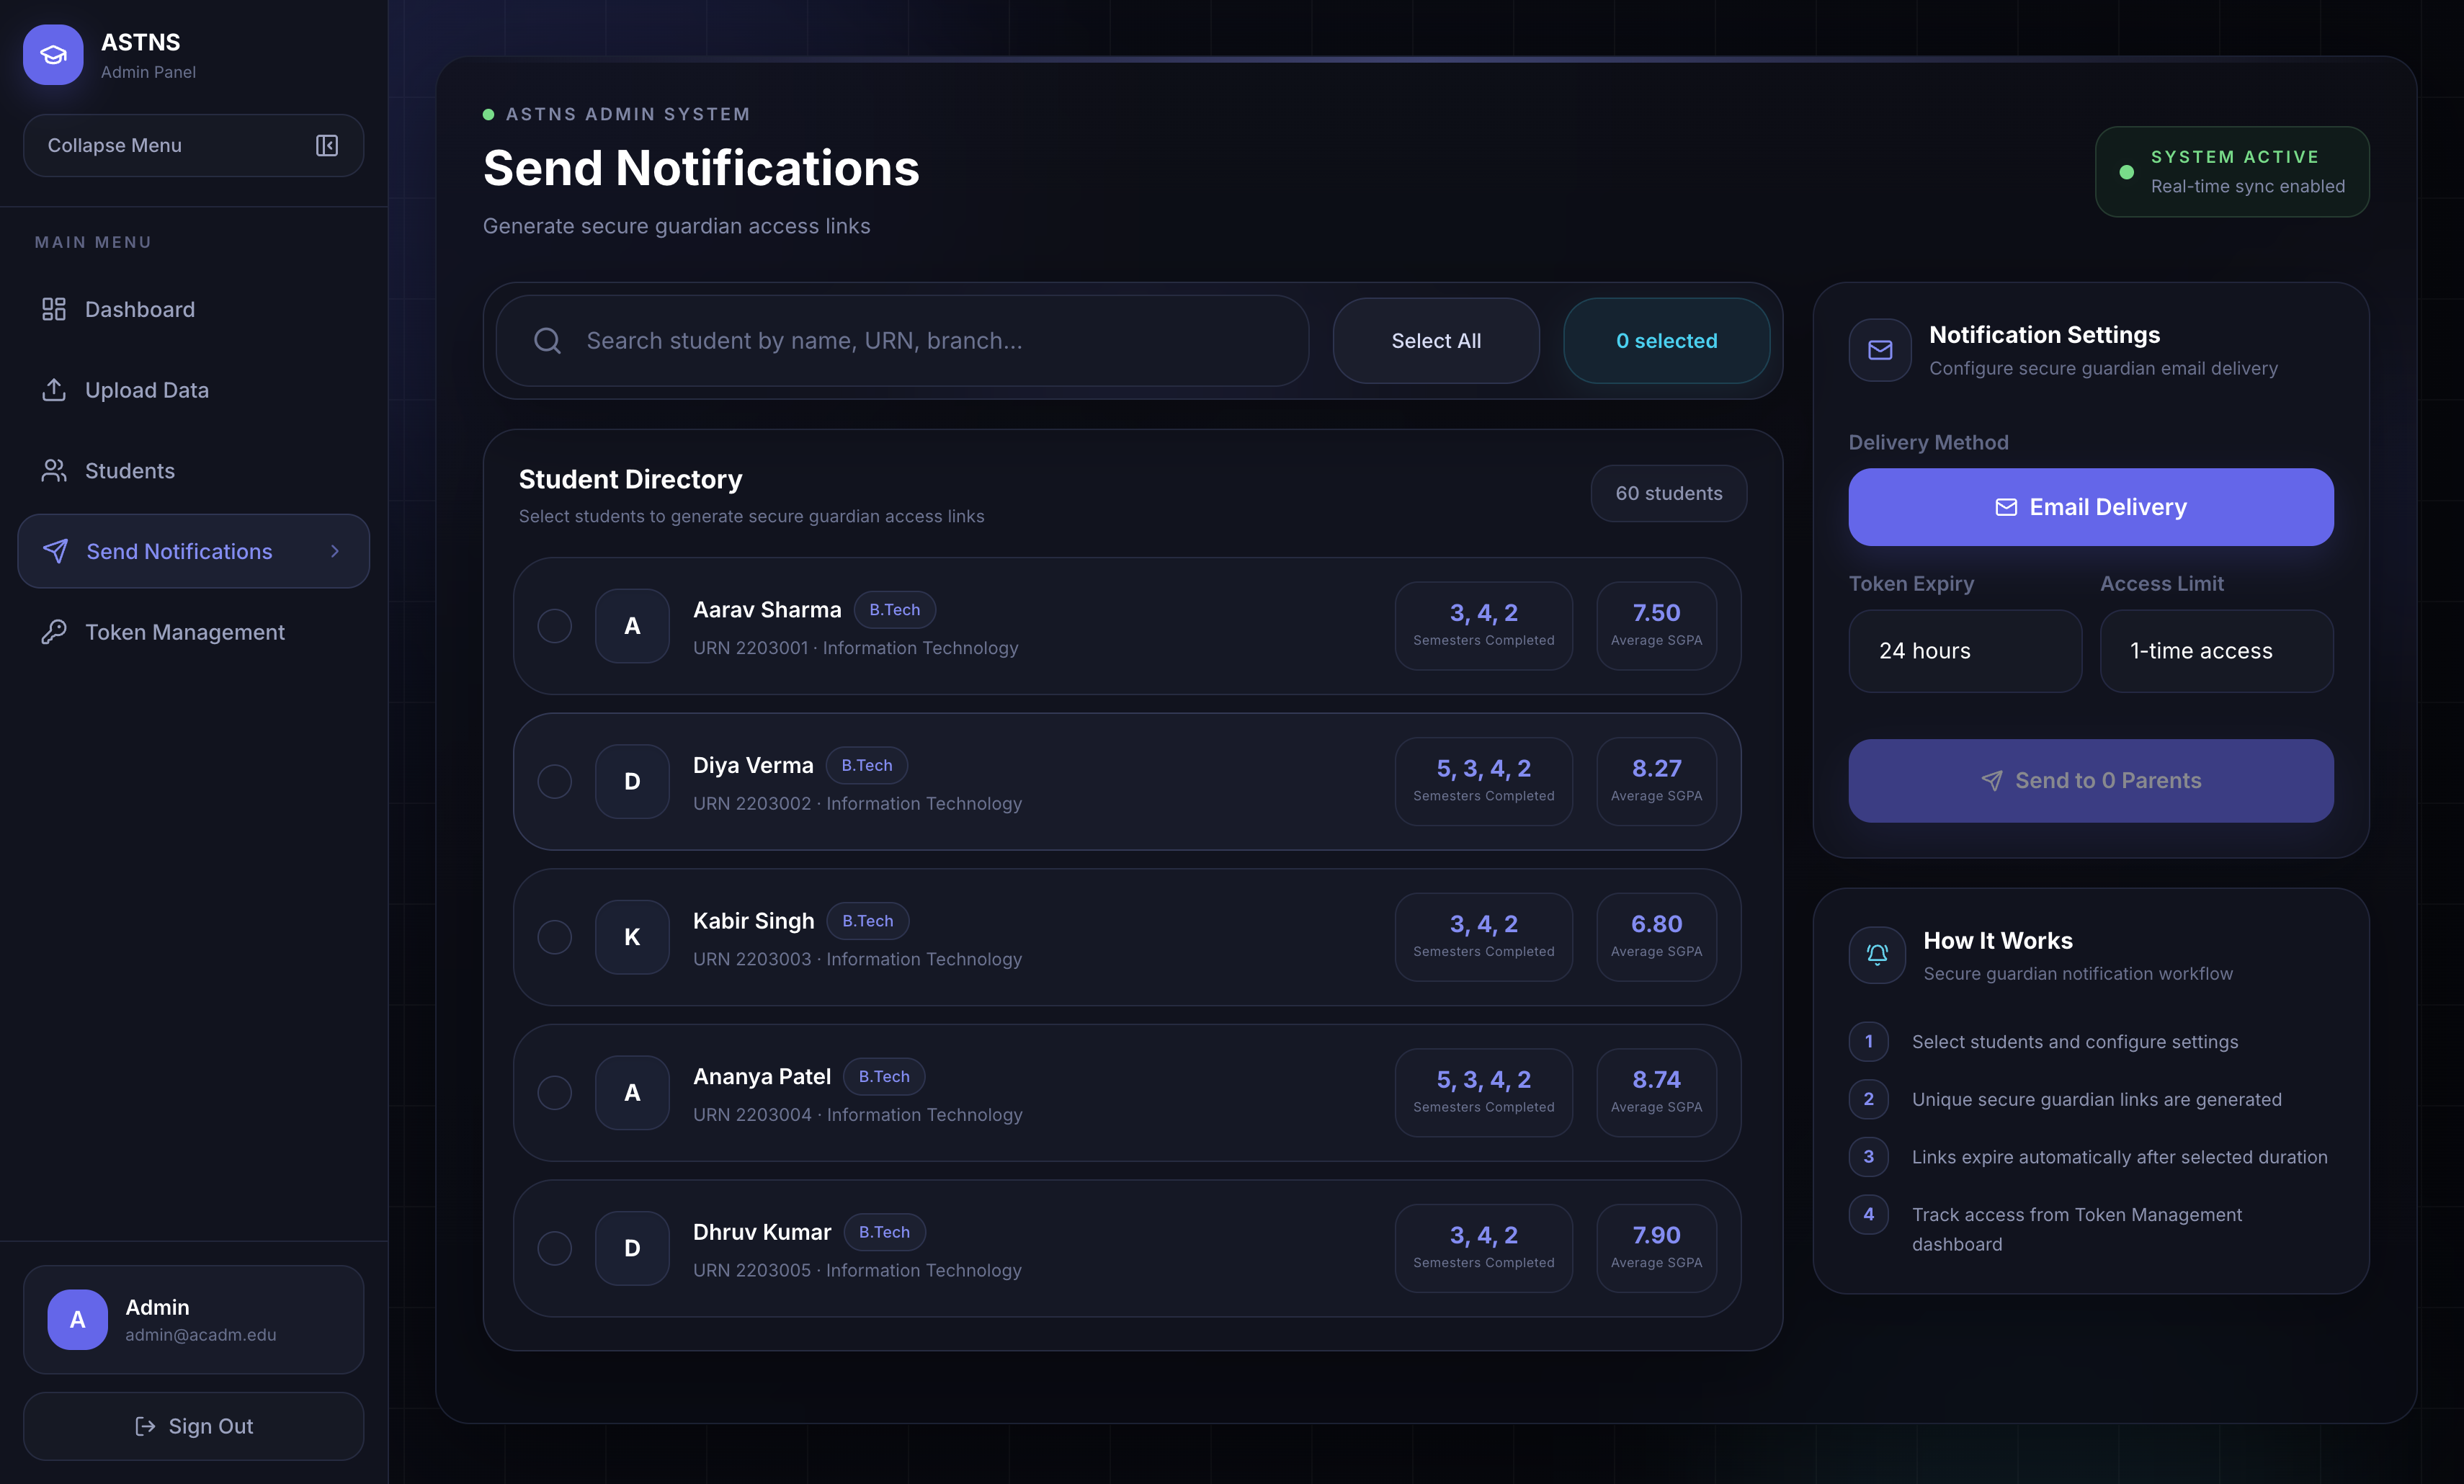
\includegraphics[width=0.85\textwidth]{assets/pic6.png}
\caption{Send Notification Page -- Bulk Email Dispatch Interface}
\end{figure}
Administrators select students via checkboxes and configure the notification parameters. Dispatch status is shown for each student after sending.

\subsection{Token Management Page}
\begin{figure}[H]
\centering
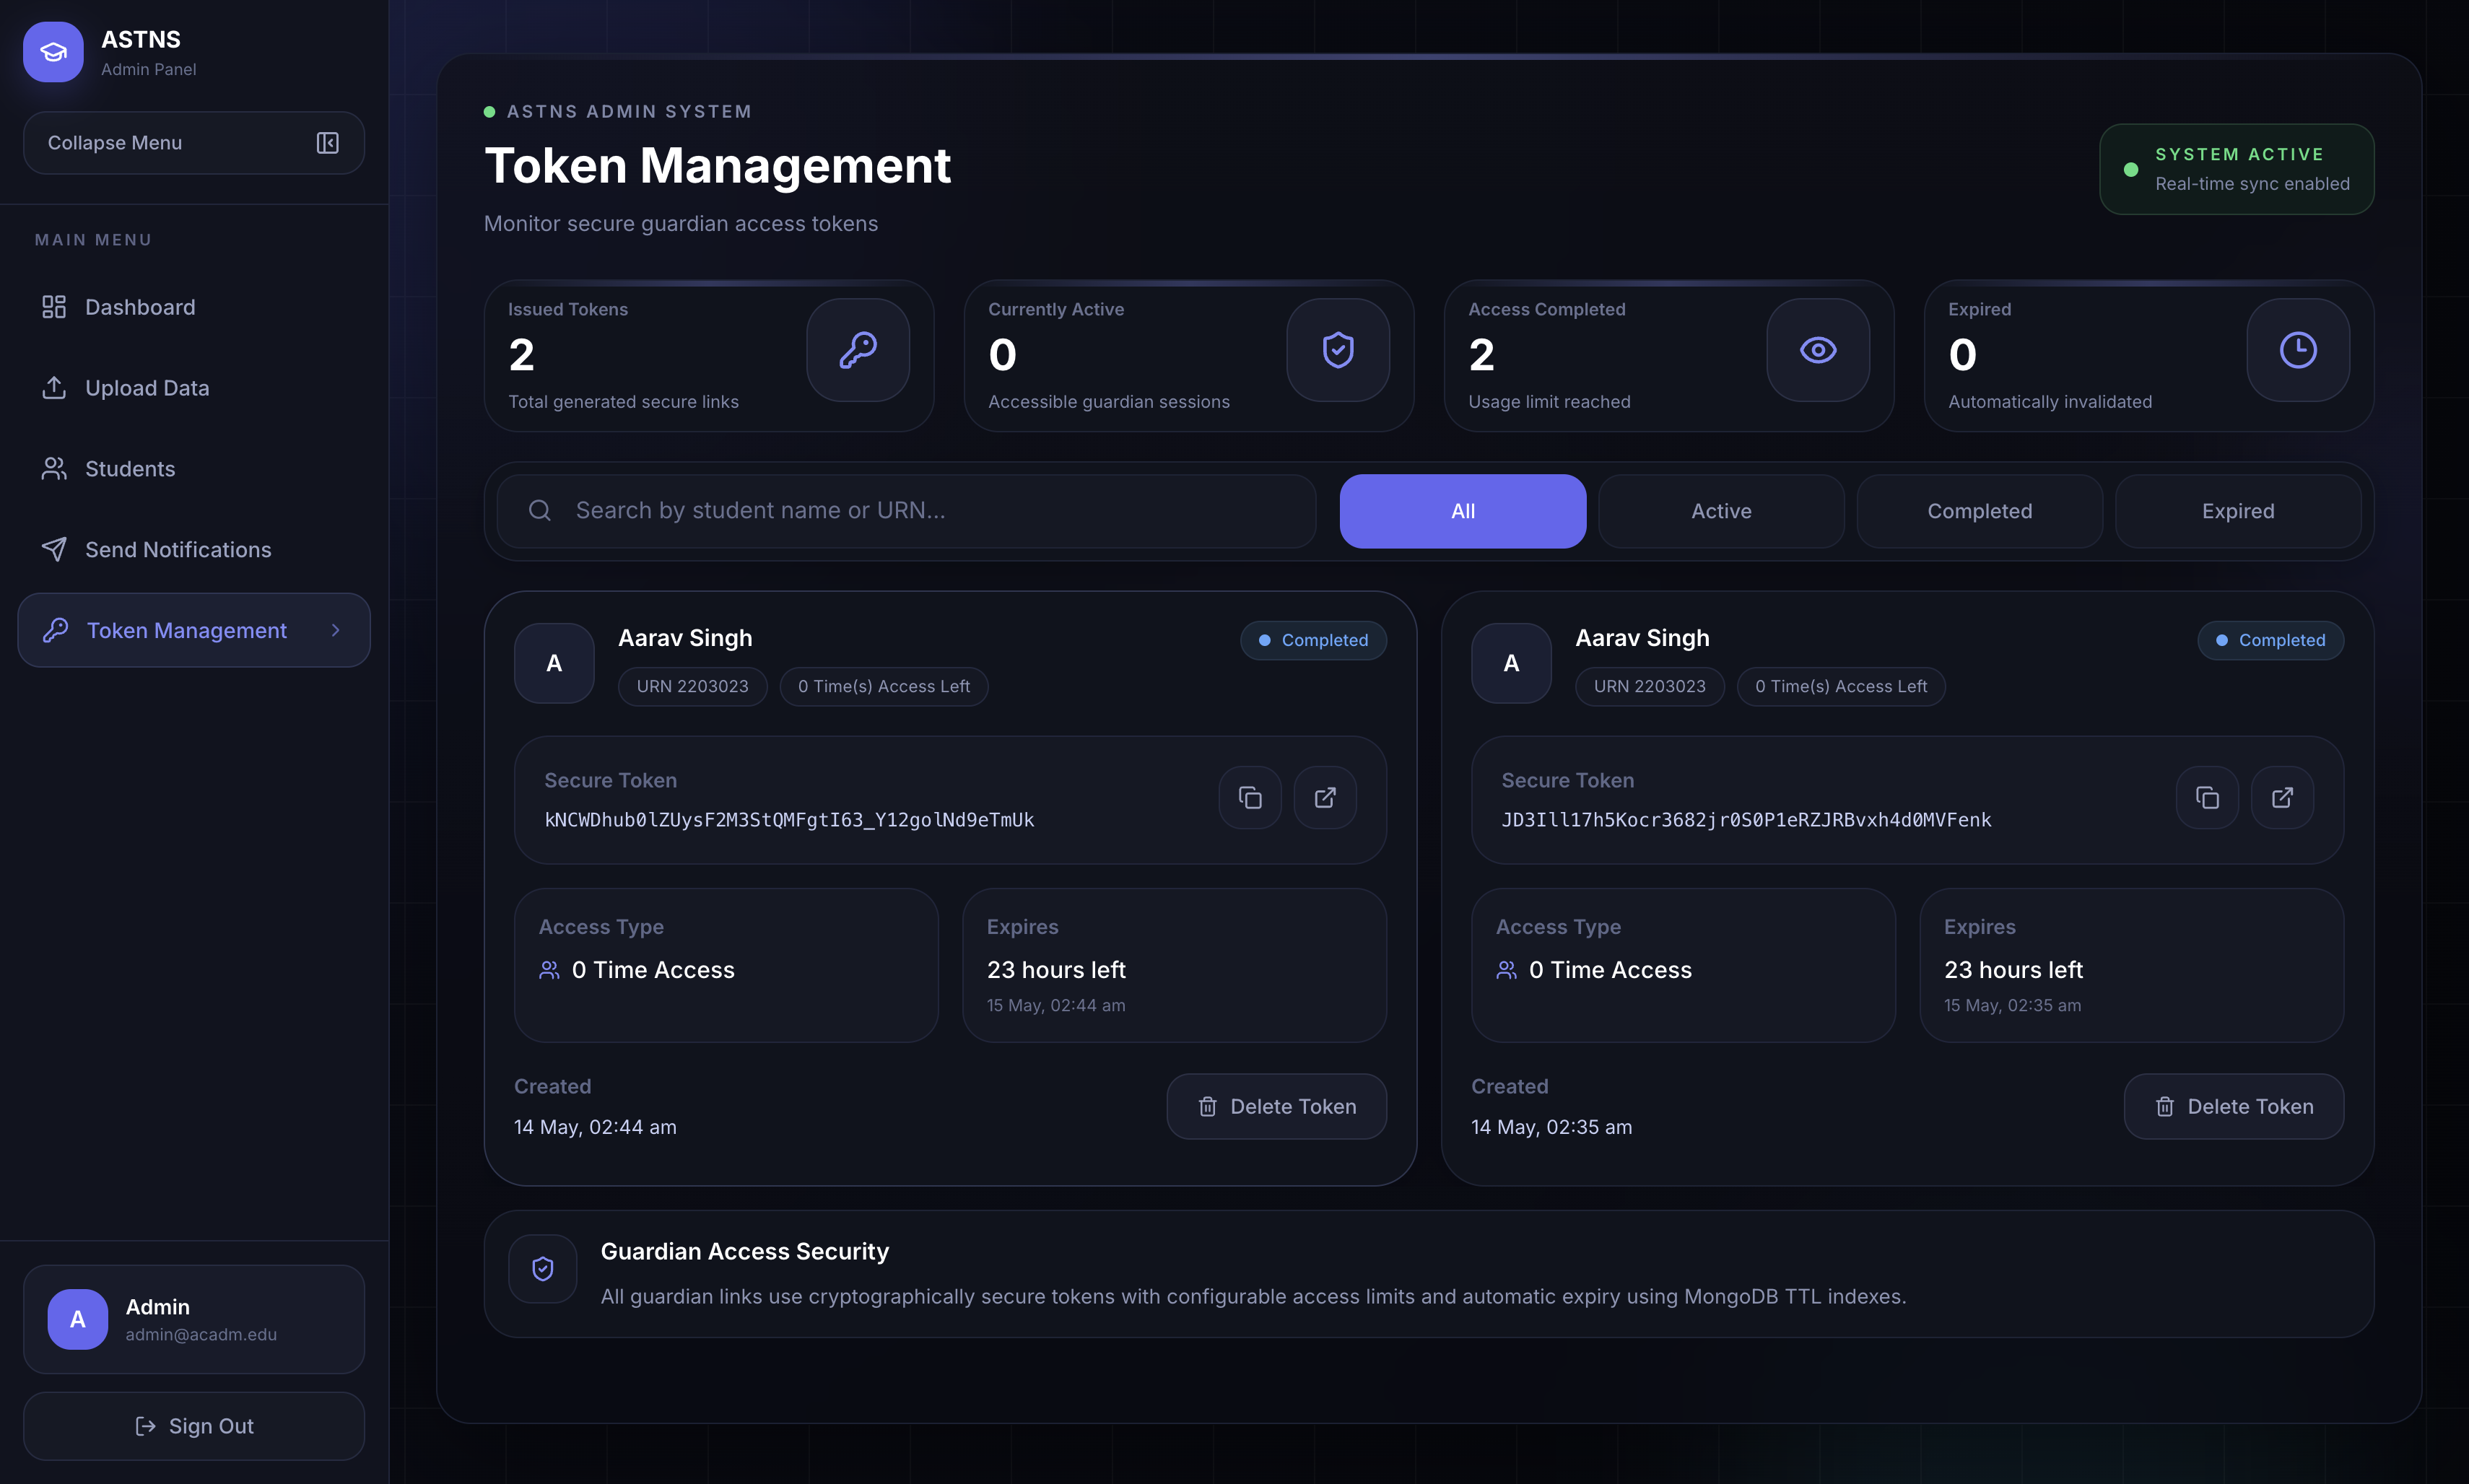
\includegraphics[width=0.85\textwidth]{assets/pic7.png}
\caption{Token Management Page -- Token Lifecycle Dashboard}
\end{figure}
All tokens are listed with their current status. Active tokens show a ``Revoke'' button. Expired tokens are greyed out.

\subsection{Guardian Dashboard -- Part 1}
\begin{figure}[H]
\centering
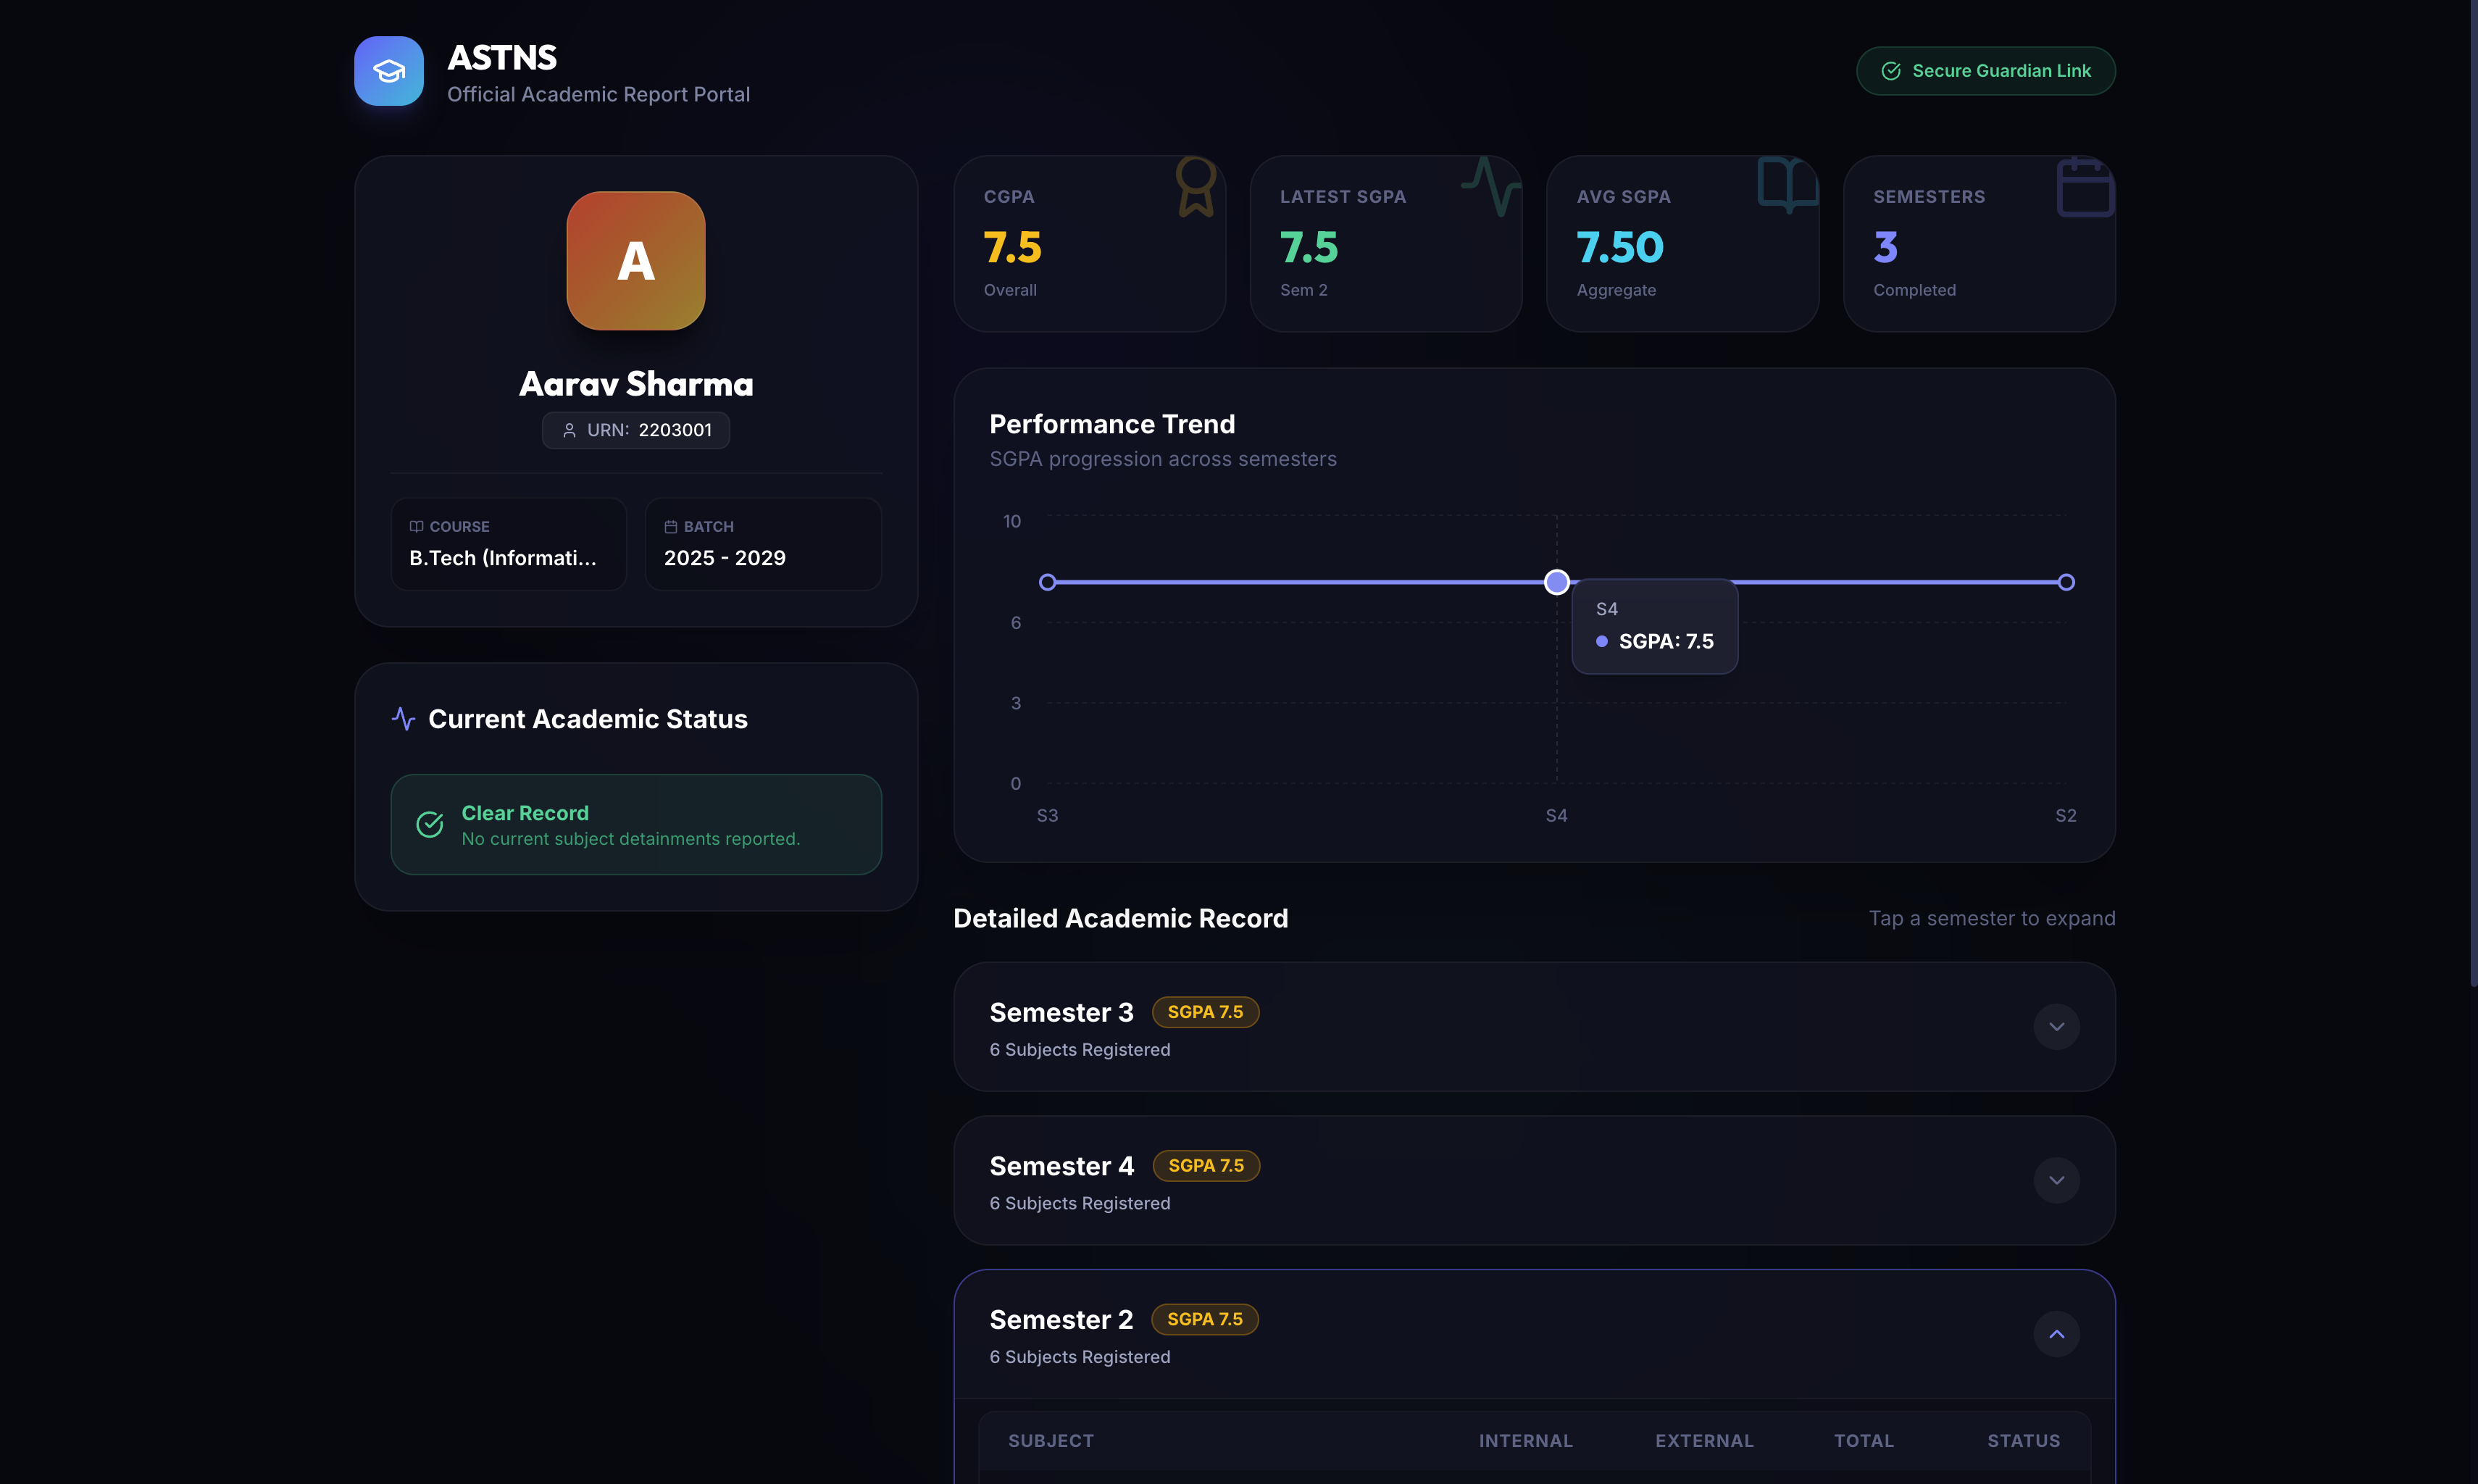
\includegraphics[width=0.85\textwidth]{assets/pic8.png}
\caption{Guardian Dashboard -- Student Profile and SGPA Chart}
\end{figure}
The Guardian Dashboard opens after token validation. The student's profile card and SGPA line chart are shown at the top of the page.

\subsection{Guardian Dashboard -- Part 2}
\begin{figure}[H]
\centering
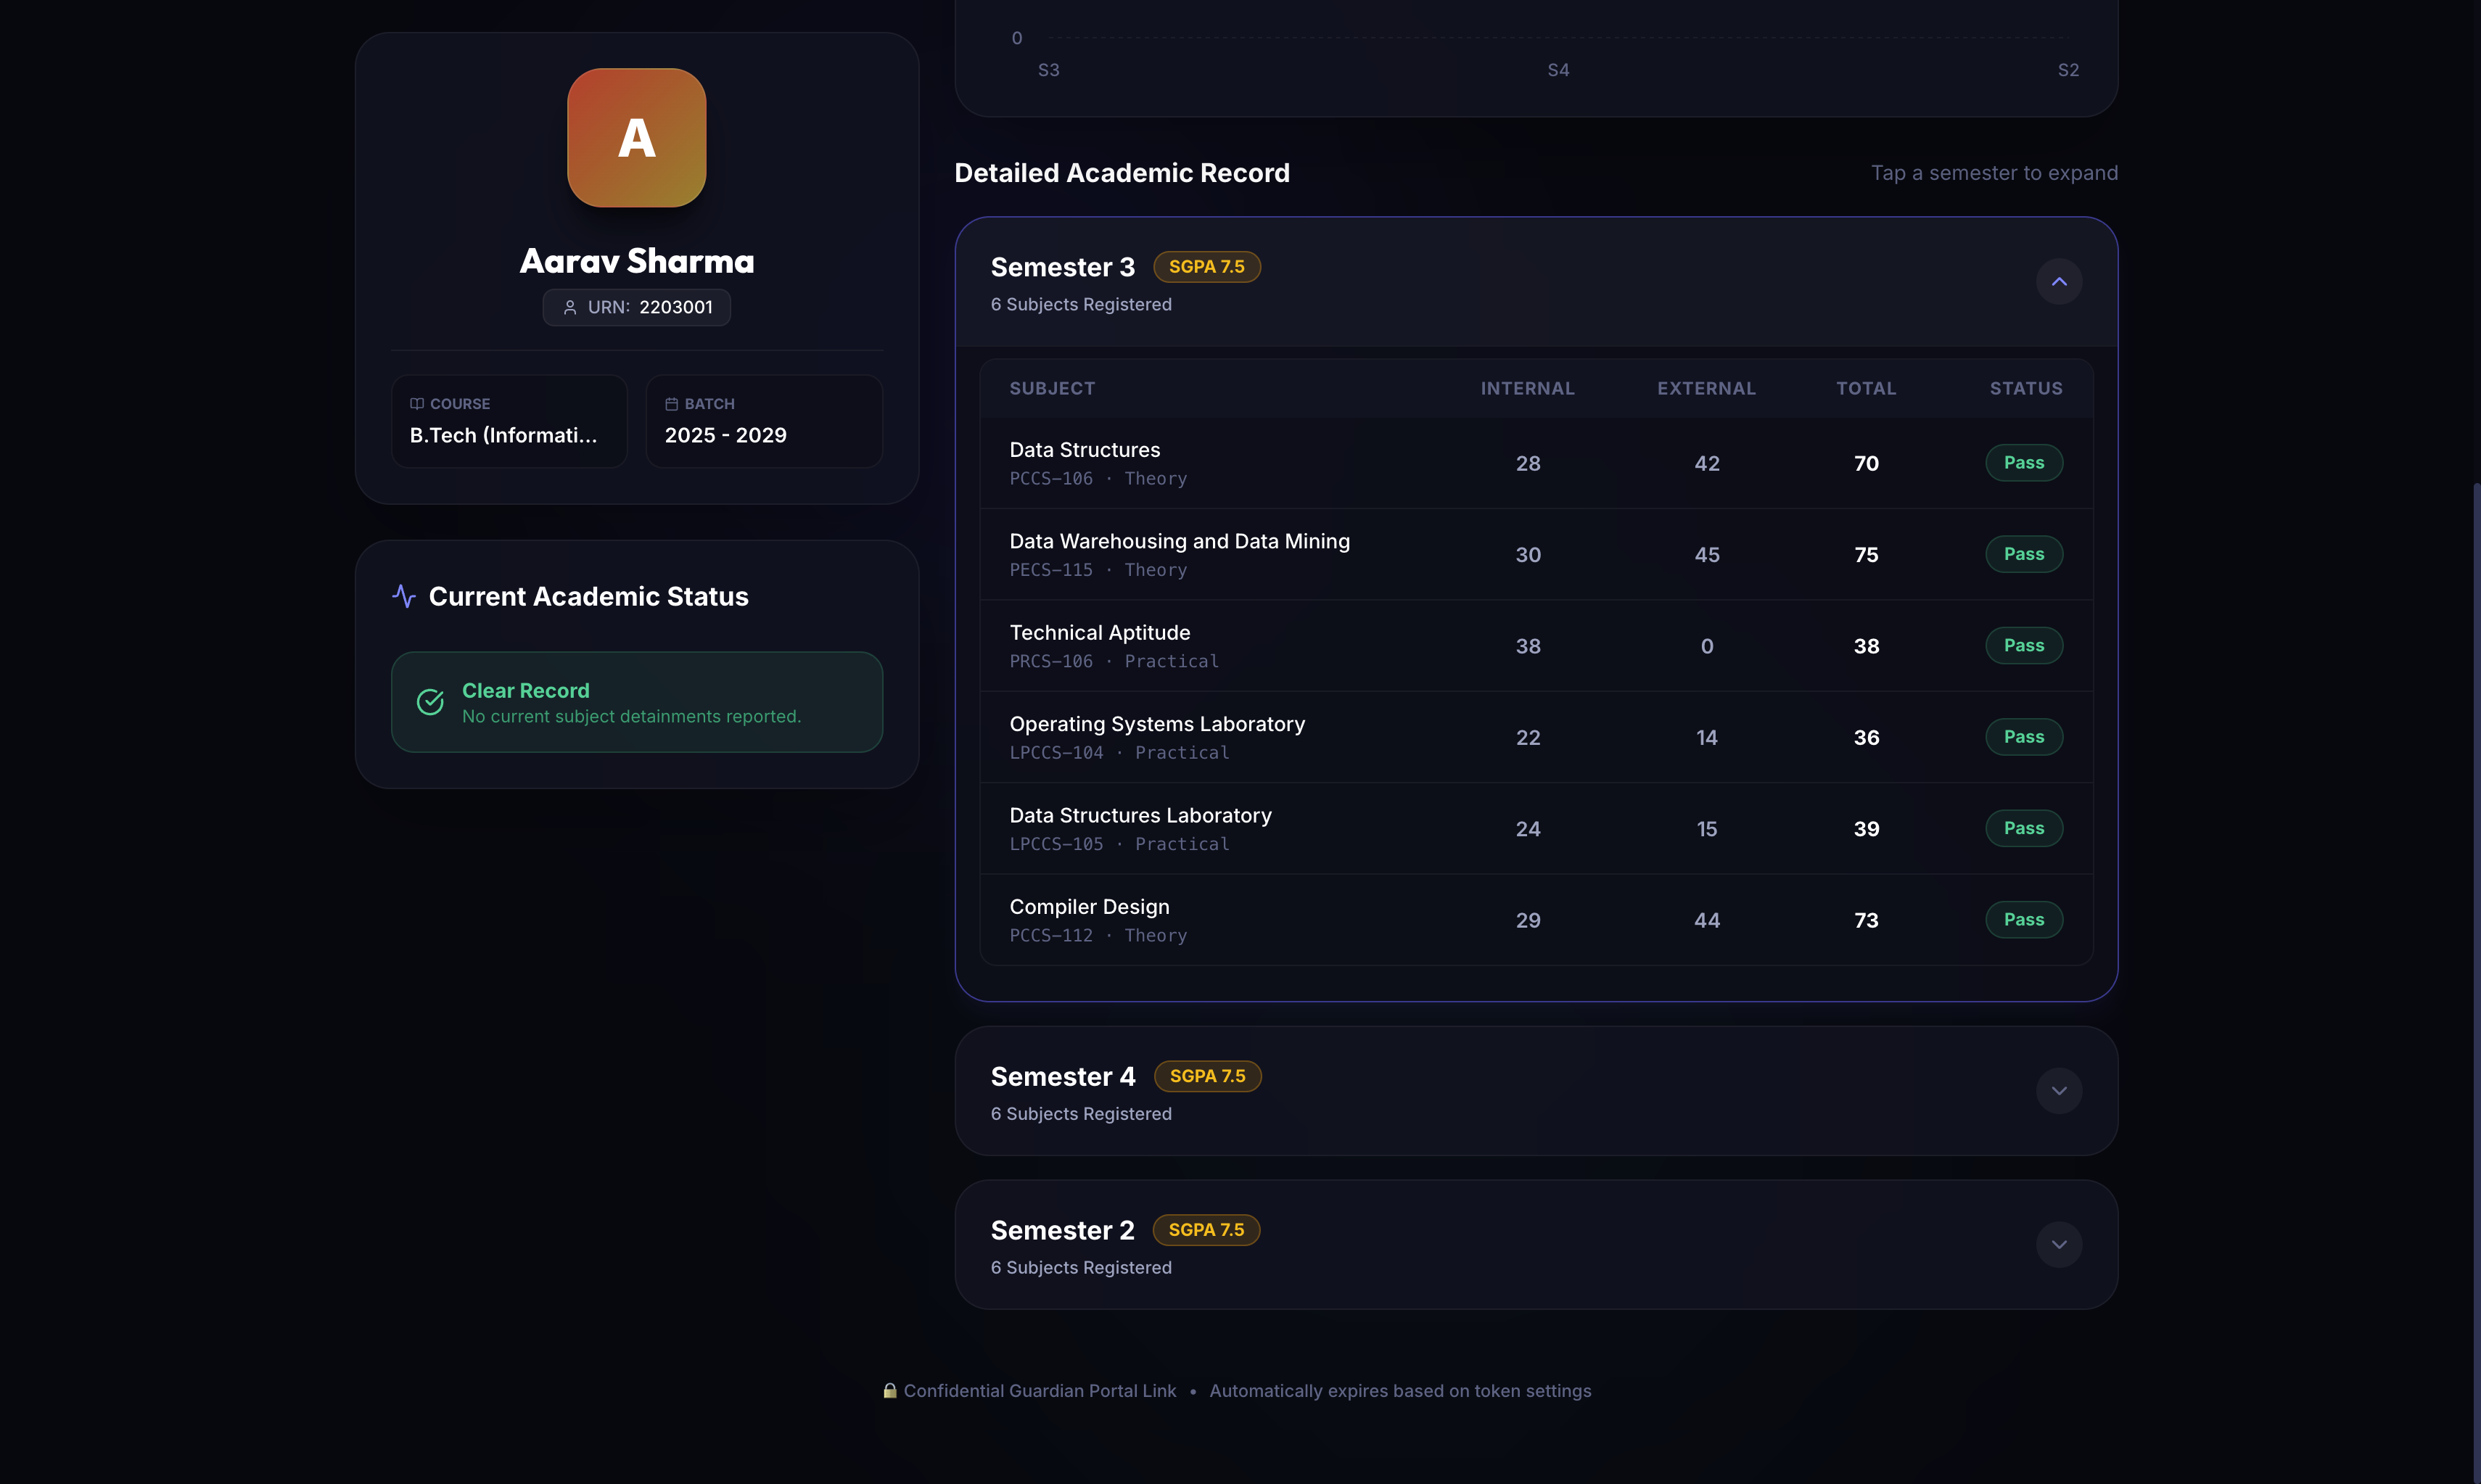
\includegraphics[width=0.85\textwidth]{assets/pic9.png}
\caption{Guardian Dashboard -- Semester-wise Mark Breakdown}
\end{figure}
Below the chart, expandable semester panels display subject-wise marks with detention status indicators.

\subsection{Access Denied Page}
\begin{figure}[H]
\centering
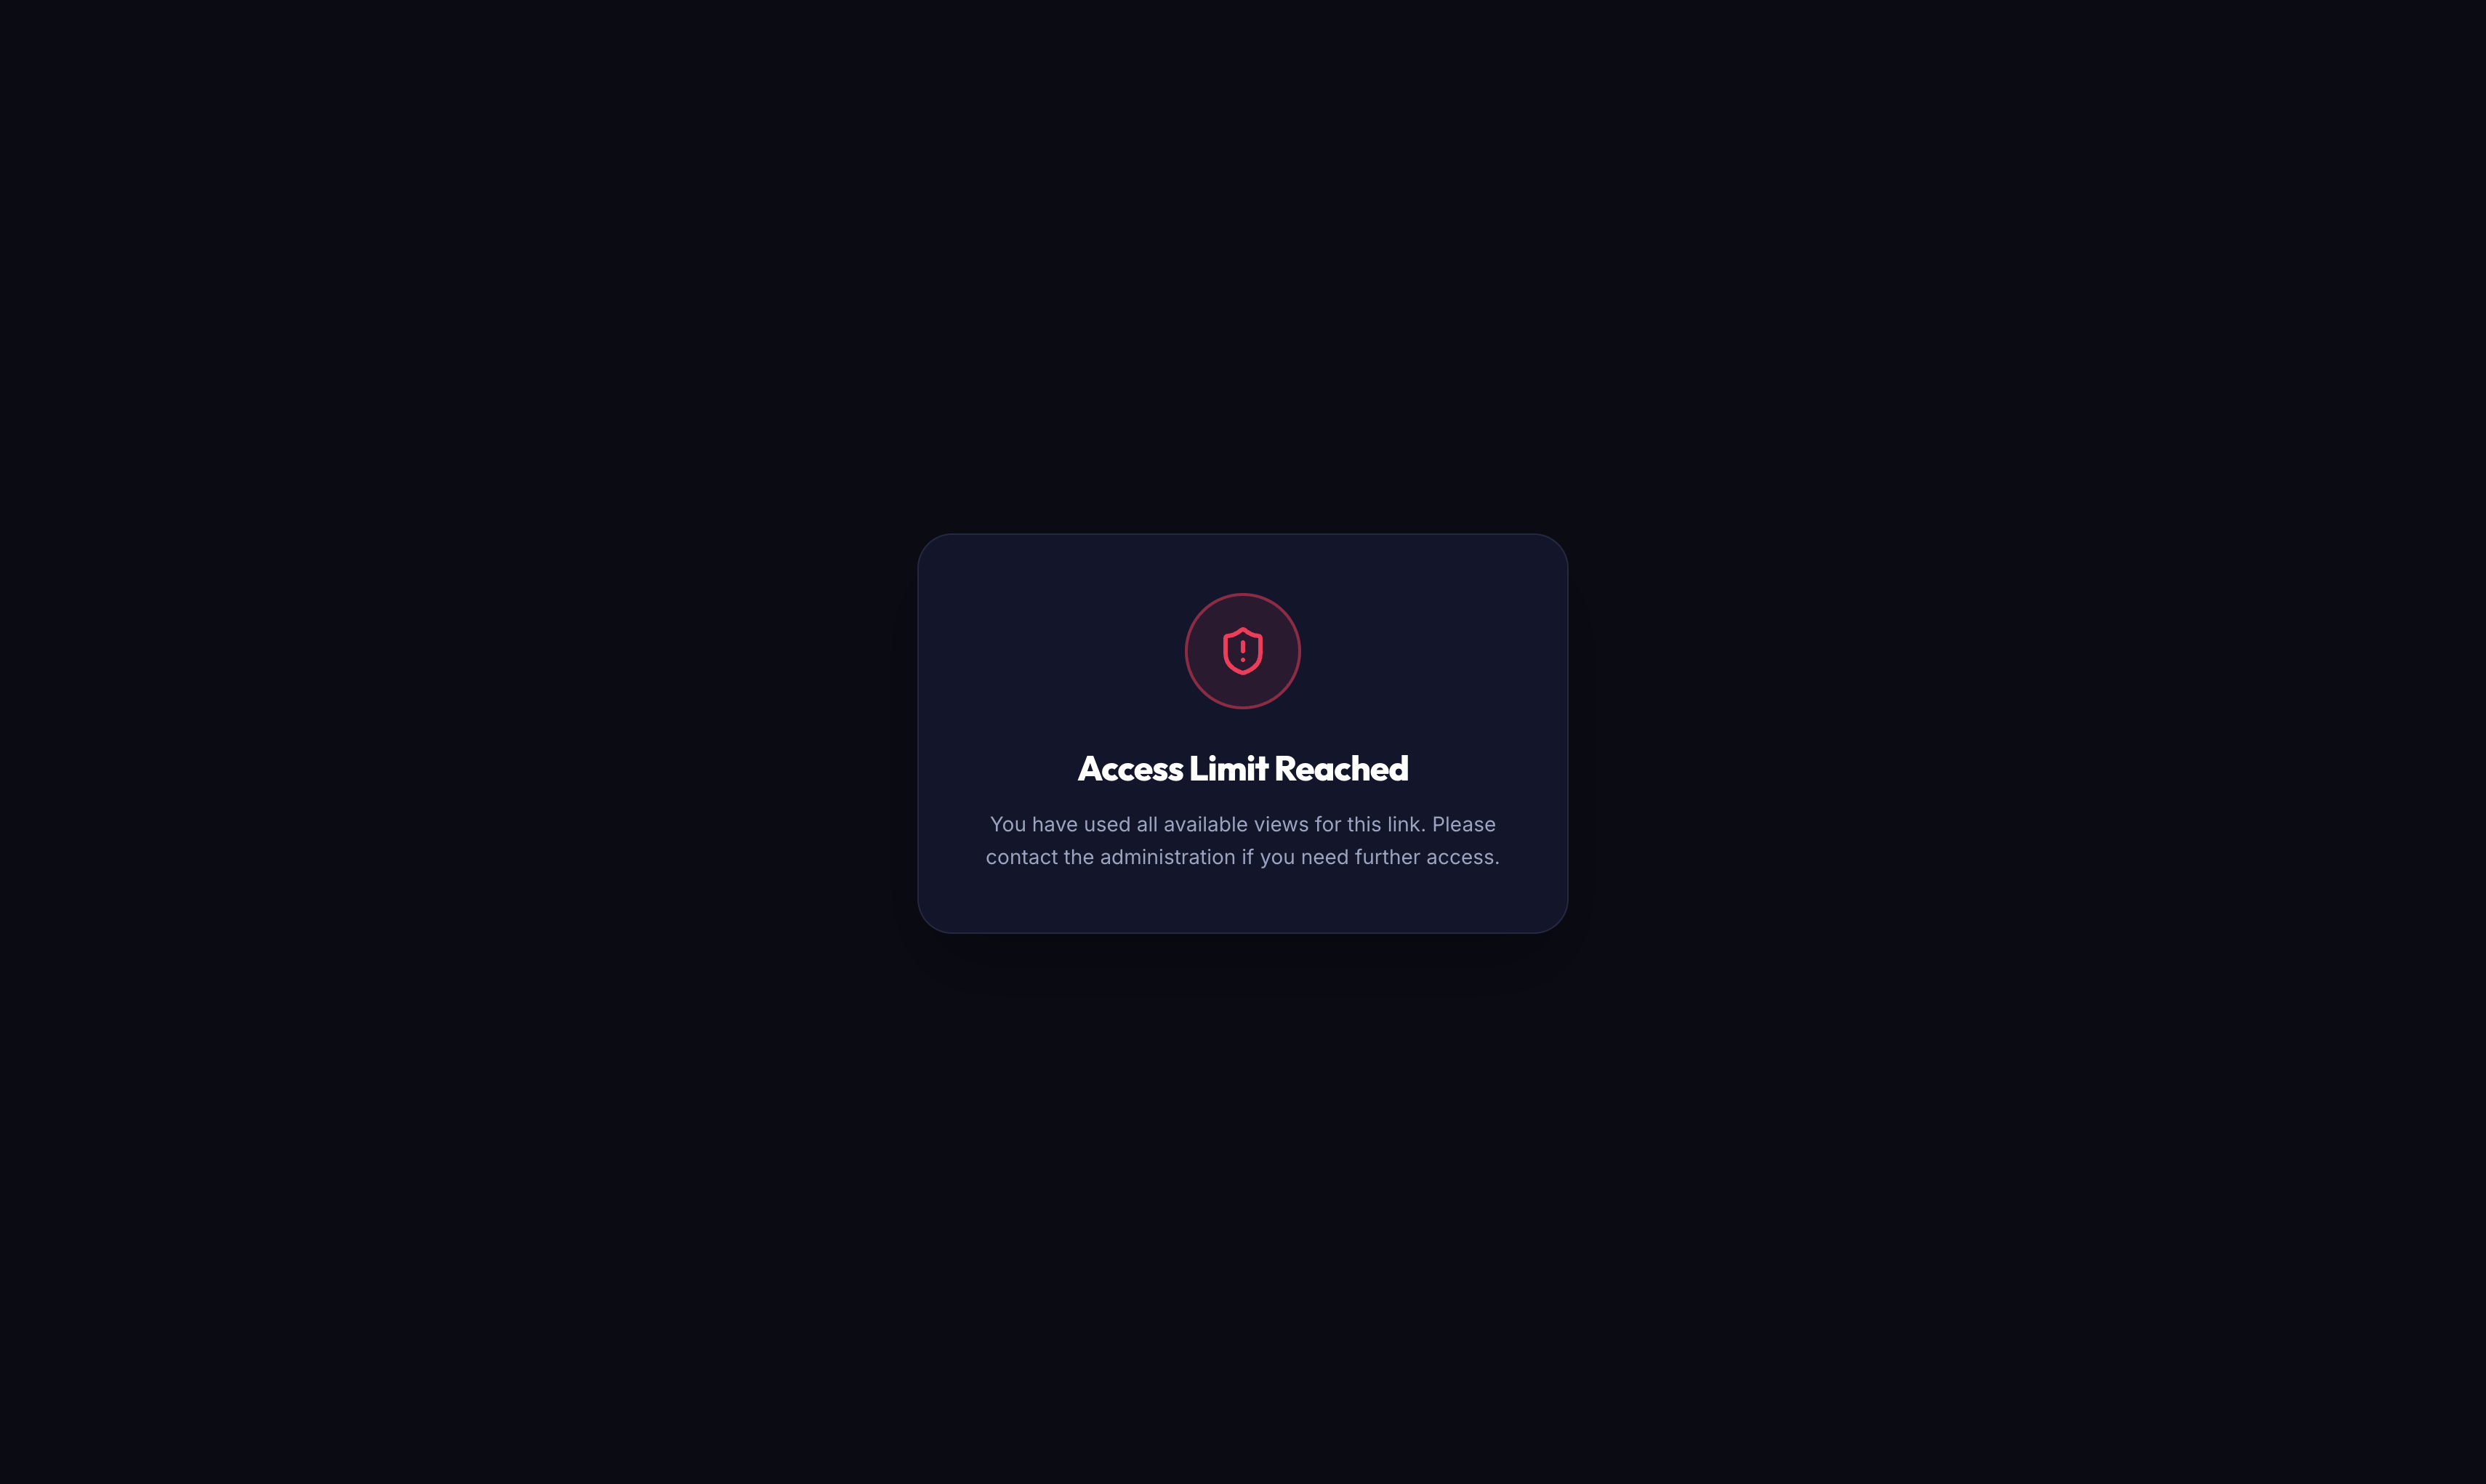
\includegraphics[width=0.85\textwidth]{assets/pic10.png}
\caption{Access Denied Page -- Expired or Revoked Token}
\end{figure}
When an invalid, expired, or revoked token is used, the Access Denied page is displayed with an appropriate explanation.

\subsection{Email Notification}
\begin{figure}[H]
\centering
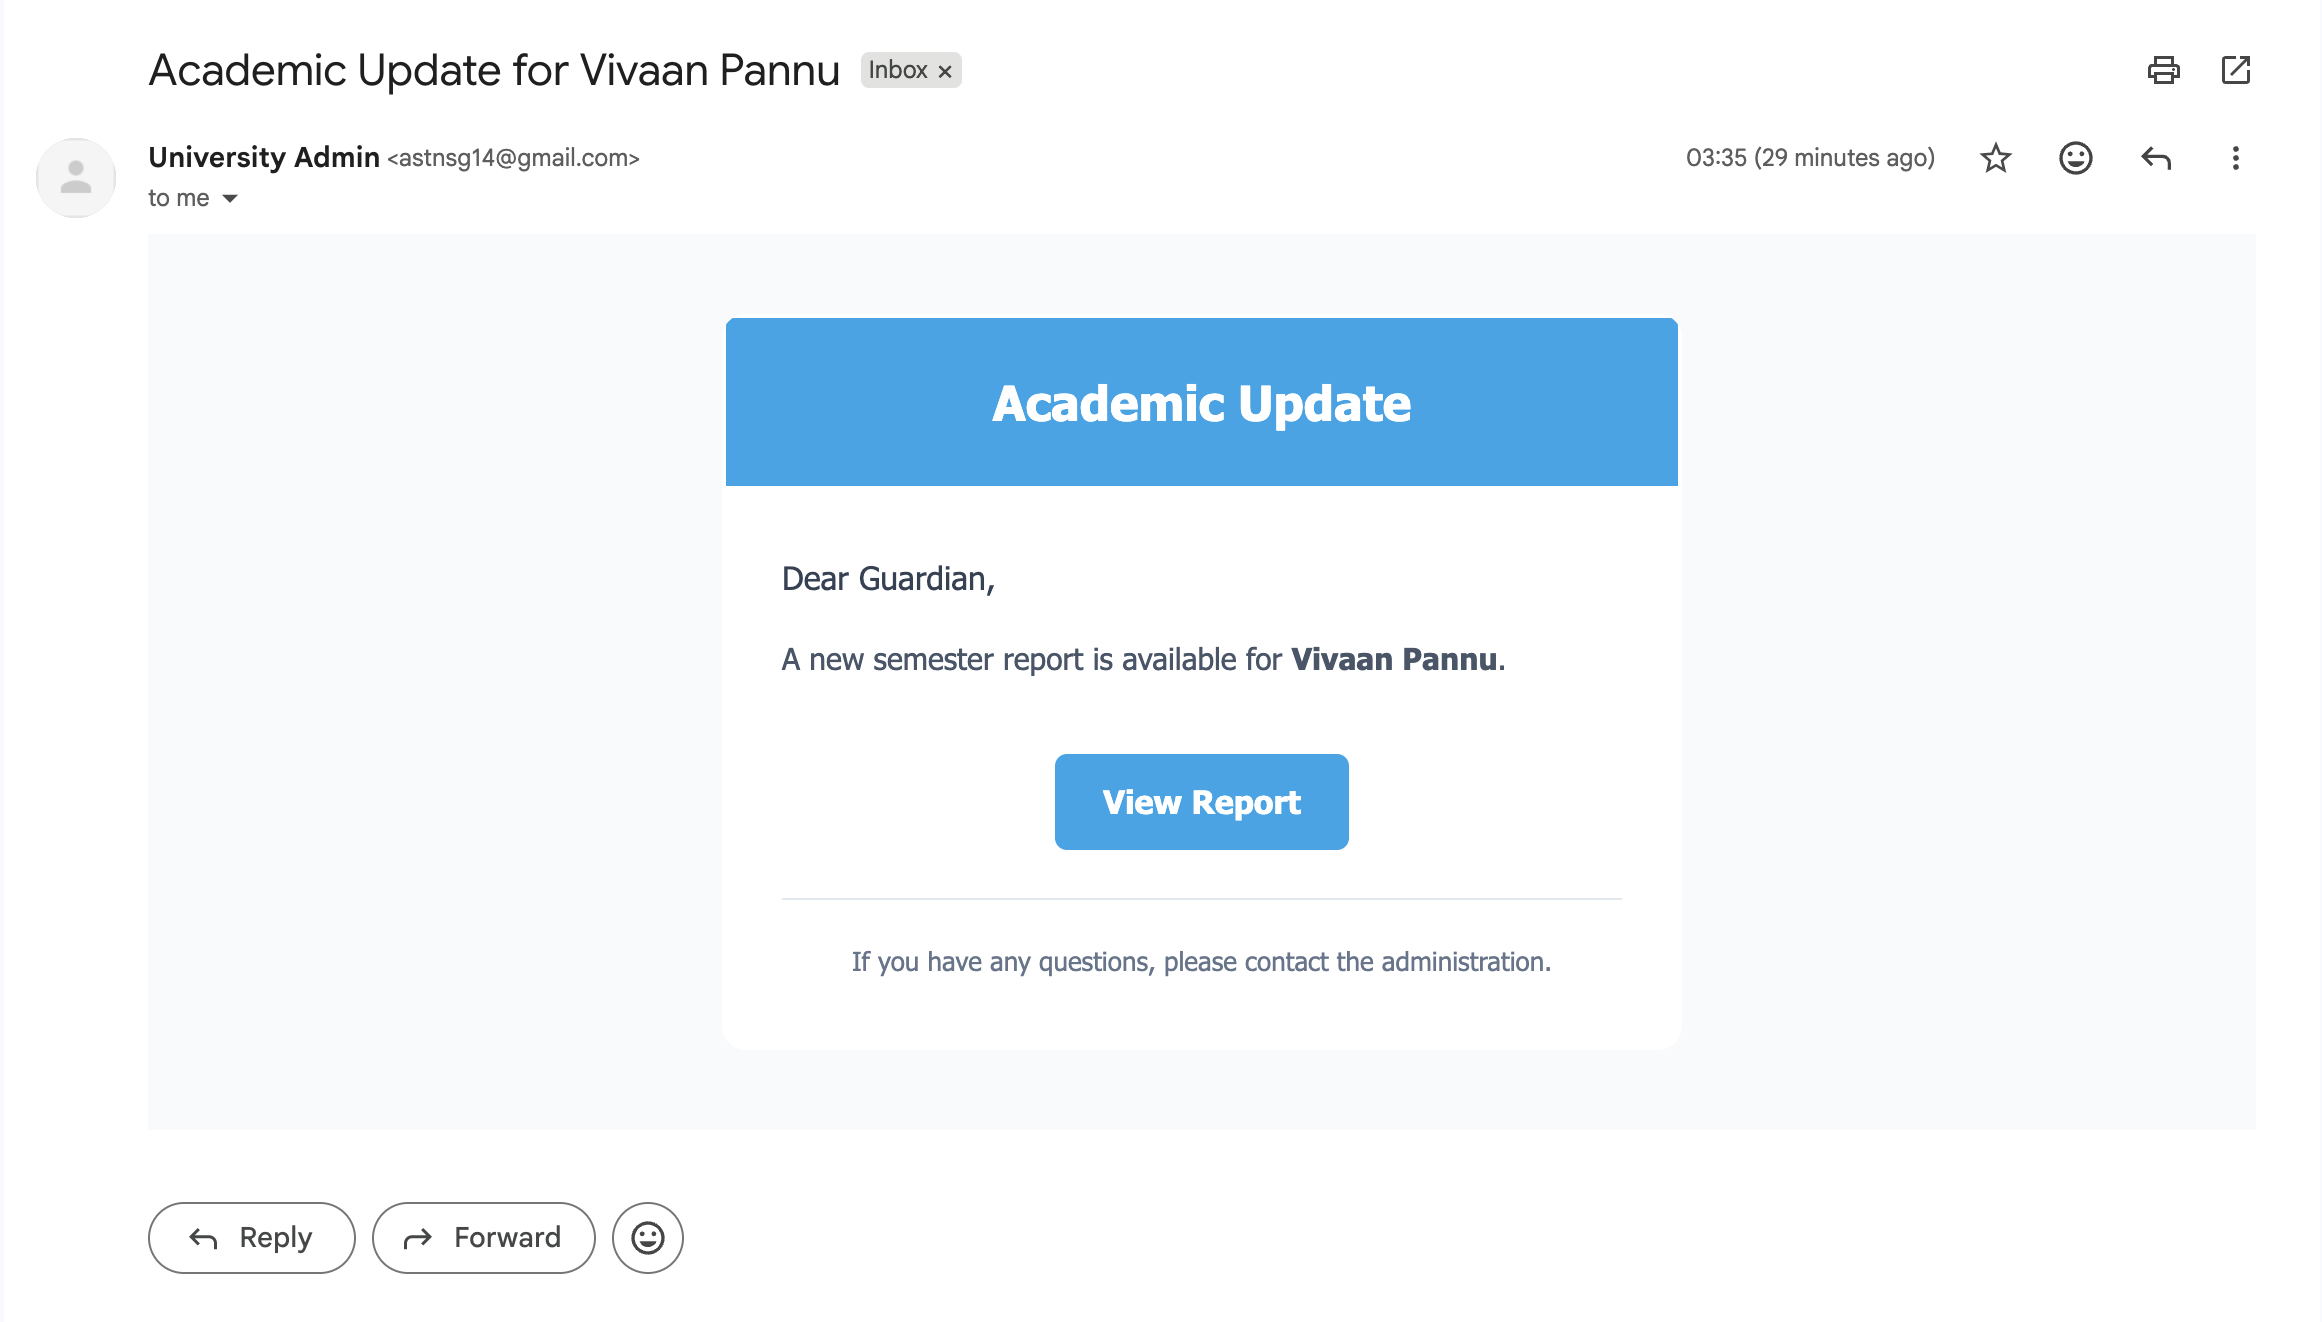
\includegraphics[width=0.85\textwidth]{assets/pic11.png}
\caption{Email Notification -- Guardian Notification Email Template}
\end{figure}
The HTML email dispatched to guardians contains a personalised greeting with the student's name, a brief description of the system, and a prominently styled ``View Report'' button linking to the Guardian Portal.

\section{Backend Database Representation}

\subsection{MongoDB Atlas Collections}
The MongoDB Atlas database for ASTNS contains the following collections:

\begin{itemize}
  \item \textbf{admins:} Stores administrator credentials. Passwords are stored as bcrypt hashes with salt rounds of 12. Each admin document contains: \texttt{userName}, \texttt{email}, \texttt{password} (hashed), and \texttt{role}.

  \item \textbf{students:} The primary collection. Each student document contains nested \texttt{semesters} arrays, and each semester contains nested \texttt{subjects} arrays (each referencing a Subject document by ObjectId). The hierarchical document structure of MongoDB is ideally suited to this nested data model.

  \item \textbf{subjects:} A reference collection storing subject master data (title, code, type, credits, max marks, pass marks). Subject records are shared across students via ObjectId references, ensuring consistency.

  \item \textbf{tokens:} Stores all generated access tokens with their lifecycle metadata (status, expiry, usedAt). Automatic expiry is enforced by querying and updating expired tokens on each token-related API call.

  \item \textbf{sessions:} Stores admin session records linked to admin ObjectIds. Session-based authentication is used instead of JWT to support server-side session invalidation on logout.
\end{itemize}

\subsection{Database Performance}
MongoDB's document model allows the complete student academic profile (all semesters, all subjects) to be fetched in a single query with \texttt{populate()}, avoiding expensive multi-table JOIN operations required in relational databases. The \texttt{lean()} option is used on read-only queries to return plain JavaScript objects instead of full Mongoose documents, improving performance by approximately 25--30\%.

\section{Discussions}
The successful implementation and deployment of ASTNS demonstrates that a modern full-stack MERN application can effectively solve a real institutional communication problem with minimal infrastructure cost.

Key findings from the testing and evaluation phase:

\begin{enumerate}
  \item \textbf{Email Deliverability:} All test emails dispatched via Gmail SMTP were successfully delivered to recipient inboxes. No emails were flagged as spam during testing, owing to the use of an authenticated Gmail account with App Password authentication.

  \item \textbf{Token Security:} The 32-character hexadecimal token space ($16^{32}$ = $2^{128}$ possible values) is computationally infeasible to brute-force, providing security equivalent to a 128-bit symmetric key.

  \item \textbf{Batch Performance:} Notification dispatch to a batch of 50 students using \texttt{Promise.all} completed within 8--12 seconds, with all emails delivered successfully. The parallel processing approach significantly outperformed sequential dispatch.

  \item \textbf{Guardian Portal Load Time:} The Guardian Portal loaded student data (including full semester and subject population) within 1.2--1.8 seconds on a standard broadband connection, meeting the 2-second performance requirement.

  \item \textbf{Cross-Browser Compatibility:} The application rendered correctly and all features functioned as expected on Chrome, Firefox, Edge, and Safari. The responsive design maintained usability on screens as small as 375px (iPhone SE viewport).

  \item \textbf{Data Integrity:} Mongoose schema validation successfully rejected all invalid data inputs during CSV upload testing, including out-of-range marks, invalid email formats, and invalid course-branch combinations.
\end{enumerate}

\chapter{Conclusion and Future Scope}

\section{Conclusion}
The Academic Status Transparency Notification System (ASTNS) successfully addresses the critical communication gap between engineering colleges and the parents or guardians of enrolled students. The system demonstrates that a well-designed full-stack web application, built on freely available open-source technologies, can deliver significant institutional value at near-zero operational cost.

The project achieved all six of its stated objectives:
\begin{enumerate}
  \item A secure, session-authenticated Admin Dashboard was designed and developed, allowing institutional administrators to manage student academic data efficiently.
  \item A bulk data upload module was implemented that accepts CSV and Excel files, validates records against strict schema constraints, and persists them to a cloud database.
  \item An automated email notification pipeline was developed that generates cryptographically secure, time-limited access tokens and dispatches personalised HTML emails to guardians.
  \item A token-authenticated Guardian Portal was created that renders a student's complete academic profile without requiring guardians to create an account.
  \item A Token Management module was implemented that allows administrators to monitor and revoke access tokens.
  \item The complete application was deployed on Vercel as a serverless application, ensuring high availability and automatic scaling.
\end{enumerate}

The system was successfully tested across all major user workflows and use cases. All functional requirements were met. The application demonstrated strong cross-browser compatibility, responsive design for mobile devices, and acceptable performance under batch notification scenarios.

The use of MongoDB's document model proved particularly advantageous for the nested, hierarchical structure of student academic data (student $\rightarrow$ semesters $\rightarrow$ subjects). The serverless deployment model eliminated infrastructure management concerns, making the system suitable for adoption by resource-constrained educational institutions.

Most importantly, ASTNS proves the concept that password-less, token-based access mechanisms borrowed from banking and e-commerce domains can be effectively applied to educational notification systems. This approach maximises guardian engagement by removing all technical barriers to accessing academic reports.

\section{Future Scope}
While the current implementation of ASTNS meets all project objectives, several enhancements can significantly extend its utility and impact:

\begin{itemize}
  \item \textbf{SMS and WhatsApp Notification:} Integrating Twilio SMS API and WhatsApp Business API would enable notification delivery via mobile messaging platforms, reaching guardians who do not actively use email. This is particularly relevant for semi-urban and rural demographics.

  \item \textbf{PDF Report Generation:} Implementing server-side PDF generation (using libraries such as Puppeteer or PDFKit) would allow guardians to download official-looking academic reports with the institution's letterhead, which could serve as documentation for official purposes.

  \item \textbf{AI-Powered Academic Risk Prediction:} Integrating a machine learning model trained on historical SGPA trends and attendance patterns could generate early warning flags for students at risk of academic failure or detention, enabling proactive intervention by both guardians and administrators.

  \item \textbf{Multi-Institution Support:} Extending the system to a multi-tenant architecture would allow multiple colleges within the IKGPTU affiliation to use a single deployment with isolated data namespaces.

  \item \textbf{Two-Way Communication:} Adding a messaging feature allowing guardians to raise academic queries or request parent-teacher meetings directly through the Guardian Portal would transform ASTNS from a one-way notification system into a comprehensive academic communication platform.

  \item \textbf{Automated Scheduled Notifications:} Implementing a CRON job-based notification scheduler (using node-cron) would allow the system to automatically dispatch notifications at configurable intervals (e.g., monthly) without requiring manual administrator action.

  \item \textbf{Localisation / Multi-language Support:} Adding support for regional languages (Hindi, Punjabi) in the Guardian Portal would make academic reports accessible to a wider demographic of parents who are more comfortable in their native languages.

  \item \textbf{Analytics Dashboard:} A comprehensive analytics module showing trends in student performance across batches, branches, and semesters would provide institutional leadership with data-driven insights for academic policy decisions.
\end{itemize}

\chapter*{References / Bibliography}
\addcontentsline{toc}{chapter}{References / Bibliography}
\begin{enumerate}
  \item C. I. P. Benablo, E. T. Sart, J. M. M. Bringula, and R. Bringula, ``An Application for Monitoring and Inquiring of Students' Academic Record with Automatic Notification for the Parents,'' \textit{International Journal of Cloud Computing and Services Science}, vol. 2, no. 1, pp. 59--66, 2014.

  \item Meta Platforms, Inc., ``React -- A JavaScript library for building user interfaces,'' 2024. [Online]. Available: \url{https://react.dev}

  \item OpenJS Foundation, ``Express.js v5 Documentation,'' 2024. [Online]. Available: \url{https://expressjs.com}

  \item MongoDB Inc., ``MongoDB Atlas Documentation,'' 2024. [Online]. Available: \url{https://www.mongodb.com/docs/atlas}

  \item Mongoose Contributors, ``Mongoose ODM v9 Documentation,'' 2024. [Online]. Available: \url{https://mongoosejs.com/docs}

  \item Nodemailer Contributors, ``Nodemailer Documentation,'' 2024. [Online]. Available: \url{https://nodemailer.com}

  \item Tailwind Labs, ``Tailwind CSS v4 Documentation,'' 2024. [Online]. Available: \url{https://tailwindcss.com/docs}

  \item Recharts Group, ``Recharts -- Redefined chart library built with React and D3,'' 2024. [Online]. Available: \url{https://recharts.org}

  \item Vercel Inc., ``Vercel Documentation -- Serverless Functions,'' 2024. [Online]. Available: \url{https://vercel.com/docs}

  \item React Hook Form Contributors, ``React Hook Form Documentation,'' 2024. [Online]. Available: \url{https://react-hook-form.com}

  \item Node.js Foundation, ``Node.js v20 LTS Documentation,'' 2024. [Online]. Available: \url{https://nodejs.org/en/docs}

  \item Vite Contributors, ``Vite Documentation,'' 2024. [Online]. Available: \url{https://vitejs.dev}

  \item I.K. Gujral Punjab Technical University, ``University Official Portal,'' 2024. [Online]. Available: \url{https://www.ptu.ac.in}

  \item GNDEC Minor Project Synopsis -- Group G14, Department of CSE, Guru Nanak Dev Engineering College, Ludhiana, 2025.
\end{enumerate}

\appendix
\chapter{Project Setup Guide}

\section{Prerequisites}
\begin{itemize}
  \item Node.js v20 LTS or higher installed.
  \item A MongoDB Atlas account with an M0 cluster created.
  \item A Gmail account with App Password generated (2FA must be enabled).
  \item Git installed.
  \item Vercel CLI installed globally (\texttt{npm install -g vercel}).
\end{itemize}

\section{Backend Setup}
\begin{verbatim}
# Clone repository
git clone https://github.com/KingArsh05/minorProjectG14.git
cd minorProjectG14/server

# Install dependencies
npm install

# Create .env file with:
MONGODB_URI=mongodb+srv://<user>:<password>@cluster.mongodb.net/astns
COOKIE_SECRET=your_cookie_secret_key
FRONTEND_URL=http://localhost:5173
SMTP_USER=yourgmail@gmail.com
SMTP_PASS=your_app_password
NODE_ENV=development

# Start development server
npm run dev
\end{verbatim}

\section{Frontend Setup}
\begin{verbatim}
cd minorProjectG14/client

# Install dependencies
npm install

# Create .env file with:
VITE_API_URL=http://localhost:3000

# Start development server
npm run dev
\end{verbatim}

\section{Deployment to Vercel}
\begin{verbatim}
# Login to Vercel
vercel login

# Deploy from project root
vercel

# Set environment variables in Vercel dashboard:
# MONGODB_URI, COOKIE_SECRET, FRONTEND_URL, SMTP_USER, SMTP_PASS
\end{verbatim}

\end{document}
